% Options for packages loaded elsewhere
\PassOptionsToPackage{unicode}{hyperref}
\PassOptionsToPackage{hyphens}{url}
\PassOptionsToPackage{dvipsnames,svgnames,x11names}{xcolor}
%
\documentclass[
  letterpaper,
  DIV=11,
  numbers=noendperiod,
  oneside]{scrreprt}

\usepackage{amsmath,amssymb}
\usepackage{iftex}
\ifPDFTeX
  \usepackage[T1]{fontenc}
  \usepackage[utf8]{inputenc}
  \usepackage{textcomp} % provide euro and other symbols
\else % if luatex or xetex
  \usepackage{unicode-math}
  \defaultfontfeatures{Scale=MatchLowercase}
  \defaultfontfeatures[\rmfamily]{Ligatures=TeX,Scale=1}
\fi
\usepackage{lmodern}
\ifPDFTeX\else  
    % xetex/luatex font selection
\fi
% Use upquote if available, for straight quotes in verbatim environments
\IfFileExists{upquote.sty}{\usepackage{upquote}}{}
\IfFileExists{microtype.sty}{% use microtype if available
  \usepackage[]{microtype}
  \UseMicrotypeSet[protrusion]{basicmath} % disable protrusion for tt fonts
}{}
\makeatletter
\@ifundefined{KOMAClassName}{% if non-KOMA class
  \IfFileExists{parskip.sty}{%
    \usepackage{parskip}
  }{% else
    \setlength{\parindent}{0pt}
    \setlength{\parskip}{6pt plus 2pt minus 1pt}}
}{% if KOMA class
  \KOMAoptions{parskip=half}}
\makeatother
\usepackage{xcolor}
\usepackage[left=1in,marginparwidth=2.0666666666667in,textwidth=4.1333333333333in,marginparsep=0.3in]{geometry}
\setlength{\emergencystretch}{3em} % prevent overfull lines
\setcounter{secnumdepth}{5}
% Make \paragraph and \subparagraph free-standing
\ifx\paragraph\undefined\else
  \let\oldparagraph\paragraph
  \renewcommand{\paragraph}[1]{\oldparagraph{#1}\mbox{}}
\fi
\ifx\subparagraph\undefined\else
  \let\oldsubparagraph\subparagraph
  \renewcommand{\subparagraph}[1]{\oldsubparagraph{#1}\mbox{}}
\fi

\usepackage{color}
\usepackage{fancyvrb}
\newcommand{\VerbBar}{|}
\newcommand{\VERB}{\Verb[commandchars=\\\{\}]}
\DefineVerbatimEnvironment{Highlighting}{Verbatim}{commandchars=\\\{\}}
% Add ',fontsize=\small' for more characters per line
\usepackage{framed}
\definecolor{shadecolor}{RGB}{241,243,245}
\newenvironment{Shaded}{\begin{snugshade}}{\end{snugshade}}
\newcommand{\AlertTok}[1]{\textcolor[rgb]{0.68,0.00,0.00}{#1}}
\newcommand{\AnnotationTok}[1]{\textcolor[rgb]{0.37,0.37,0.37}{#1}}
\newcommand{\AttributeTok}[1]{\textcolor[rgb]{0.40,0.45,0.13}{#1}}
\newcommand{\BaseNTok}[1]{\textcolor[rgb]{0.68,0.00,0.00}{#1}}
\newcommand{\BuiltInTok}[1]{\textcolor[rgb]{0.00,0.23,0.31}{#1}}
\newcommand{\CharTok}[1]{\textcolor[rgb]{0.13,0.47,0.30}{#1}}
\newcommand{\CommentTok}[1]{\textcolor[rgb]{0.37,0.37,0.37}{#1}}
\newcommand{\CommentVarTok}[1]{\textcolor[rgb]{0.37,0.37,0.37}{\textit{#1}}}
\newcommand{\ConstantTok}[1]{\textcolor[rgb]{0.56,0.35,0.01}{#1}}
\newcommand{\ControlFlowTok}[1]{\textcolor[rgb]{0.00,0.23,0.31}{#1}}
\newcommand{\DataTypeTok}[1]{\textcolor[rgb]{0.68,0.00,0.00}{#1}}
\newcommand{\DecValTok}[1]{\textcolor[rgb]{0.68,0.00,0.00}{#1}}
\newcommand{\DocumentationTok}[1]{\textcolor[rgb]{0.37,0.37,0.37}{\textit{#1}}}
\newcommand{\ErrorTok}[1]{\textcolor[rgb]{0.68,0.00,0.00}{#1}}
\newcommand{\ExtensionTok}[1]{\textcolor[rgb]{0.00,0.23,0.31}{#1}}
\newcommand{\FloatTok}[1]{\textcolor[rgb]{0.68,0.00,0.00}{#1}}
\newcommand{\FunctionTok}[1]{\textcolor[rgb]{0.28,0.35,0.67}{#1}}
\newcommand{\ImportTok}[1]{\textcolor[rgb]{0.00,0.46,0.62}{#1}}
\newcommand{\InformationTok}[1]{\textcolor[rgb]{0.37,0.37,0.37}{#1}}
\newcommand{\KeywordTok}[1]{\textcolor[rgb]{0.00,0.23,0.31}{#1}}
\newcommand{\NormalTok}[1]{\textcolor[rgb]{0.00,0.23,0.31}{#1}}
\newcommand{\OperatorTok}[1]{\textcolor[rgb]{0.37,0.37,0.37}{#1}}
\newcommand{\OtherTok}[1]{\textcolor[rgb]{0.00,0.23,0.31}{#1}}
\newcommand{\PreprocessorTok}[1]{\textcolor[rgb]{0.68,0.00,0.00}{#1}}
\newcommand{\RegionMarkerTok}[1]{\textcolor[rgb]{0.00,0.23,0.31}{#1}}
\newcommand{\SpecialCharTok}[1]{\textcolor[rgb]{0.37,0.37,0.37}{#1}}
\newcommand{\SpecialStringTok}[1]{\textcolor[rgb]{0.13,0.47,0.30}{#1}}
\newcommand{\StringTok}[1]{\textcolor[rgb]{0.13,0.47,0.30}{#1}}
\newcommand{\VariableTok}[1]{\textcolor[rgb]{0.07,0.07,0.07}{#1}}
\newcommand{\VerbatimStringTok}[1]{\textcolor[rgb]{0.13,0.47,0.30}{#1}}
\newcommand{\WarningTok}[1]{\textcolor[rgb]{0.37,0.37,0.37}{\textit{#1}}}

\providecommand{\tightlist}{%
  \setlength{\itemsep}{0pt}\setlength{\parskip}{0pt}}\usepackage{longtable,booktabs,array}
\usepackage{calc} % for calculating minipage widths
% Correct order of tables after \paragraph or \subparagraph
\usepackage{etoolbox}
\makeatletter
\patchcmd\longtable{\par}{\if@noskipsec\mbox{}\fi\par}{}{}
\makeatother
% Allow footnotes in longtable head/foot
\IfFileExists{footnotehyper.sty}{\usepackage{footnotehyper}}{\usepackage{footnote}}
\makesavenoteenv{longtable}
\usepackage{graphicx}
\makeatletter
\def\maxwidth{\ifdim\Gin@nat@width>\linewidth\linewidth\else\Gin@nat@width\fi}
\def\maxheight{\ifdim\Gin@nat@height>\textheight\textheight\else\Gin@nat@height\fi}
\makeatother
% Scale images if necessary, so that they will not overflow the page
% margins by default, and it is still possible to overwrite the defaults
% using explicit options in \includegraphics[width, height, ...]{}
\setkeys{Gin}{width=\maxwidth,height=\maxheight,keepaspectratio}
% Set default figure placement to htbp
\makeatletter
\def\fps@figure{htbp}
\makeatother

\KOMAoption{captions}{tableheading}
\makeatletter
\makeatother
\makeatletter
\@ifpackageloaded{bookmark}{}{\usepackage{bookmark}}
\makeatother
\makeatletter
\@ifpackageloaded{caption}{}{\usepackage{caption}}
\AtBeginDocument{%
\ifdefined\contentsname
  \renewcommand*\contentsname{Table of contents}
\else
  \newcommand\contentsname{Table of contents}
\fi
\ifdefined\listfigurename
  \renewcommand*\listfigurename{List of Figures}
\else
  \newcommand\listfigurename{List of Figures}
\fi
\ifdefined\listtablename
  \renewcommand*\listtablename{List of Tables}
\else
  \newcommand\listtablename{List of Tables}
\fi
\ifdefined\figurename
  \renewcommand*\figurename{Figure}
\else
  \newcommand\figurename{Figure}
\fi
\ifdefined\tablename
  \renewcommand*\tablename{Table}
\else
  \newcommand\tablename{Table}
\fi
}
\@ifpackageloaded{float}{}{\usepackage{float}}
\floatstyle{ruled}
\@ifundefined{c@chapter}{\newfloat{codelisting}{h}{lop}}{\newfloat{codelisting}{h}{lop}[chapter]}
\floatname{codelisting}{Listing}
\newcommand*\listoflistings{\listof{codelisting}{List of Listings}}
\makeatother
\makeatletter
\@ifpackageloaded{caption}{}{\usepackage{caption}}
\@ifpackageloaded{subcaption}{}{\usepackage{subcaption}}
\makeatother
\makeatletter
\@ifpackageloaded{tcolorbox}{}{\usepackage[skins,breakable]{tcolorbox}}
\makeatother
\makeatletter
\@ifundefined{shadecolor}{\definecolor{shadecolor}{rgb}{.97, .97, .97}}
\makeatother
\makeatletter
\makeatother
\makeatletter
\@ifpackageloaded{sidenotes}{}{\usepackage{sidenotes}}
\@ifpackageloaded{marginnote}{}{\usepackage{marginnote}}
\makeatother
\makeatletter
\makeatother
\ifLuaTeX
  \usepackage{selnolig}  % disable illegal ligatures
\fi
\IfFileExists{bookmark.sty}{\usepackage{bookmark}}{\usepackage{hyperref}}
\IfFileExists{xurl.sty}{\usepackage{xurl}}{} % add URL line breaks if available
\urlstyle{same} % disable monospaced font for URLs
\hypersetup{
  pdftitle={OBIS Manual},
  colorlinks=true,
  linkcolor={blue},
  filecolor={Maroon},
  citecolor={Blue},
  urlcolor={Blue},
  pdfcreator={LaTeX via pandoc}}

\title{OBIS Manual}
\author{}
\date{}

\begin{document}
\maketitle
\ifdefined\Shaded\renewenvironment{Shaded}{\begin{tcolorbox}[borderline west={3pt}{0pt}{shadecolor}, interior hidden, breakable, enhanced, boxrule=0pt, sharp corners, frame hidden]}{\end{tcolorbox}}\fi

\renewcommand*\contentsname{Table of contents}
{
\hypersetup{linkcolor=}
\setcounter{tocdepth}{2}
\tableofcontents
}
\bookmarksetup{startatroot}

\hypertarget{making-better-use-of-obis-data}{%
\chapter*{Making better use of OBIS
data}\label{making-better-use-of-obis-data}}
\addcontentsline{toc}{chapter}{Making better use of OBIS data}

\markboth{Making better use of OBIS data}{Making better use of OBIS
data}

OBIS is not just a repository for biodiversity data. It's also a
community of practice that want to leverage the use of ocean
biodiversity data. Here you will find tutorials and tools to help you
make better use of data from OBIS (and other resources).

You can contribute with tutorials following the guidelines available
\href{https://github.com/iobis/resources}{at our repository}.

Don't know where to start? We suggest reading the
\href{https://manual.obis.org/}{OBIS manual} where you will find the
most complete guide about how OBIS works and the different types of data
available.

Check also the available
\href{https://resources.obis.org/packages/}{packages and pipelines} for
R and other languages, and
\href{https://resources.obis.org/find-your-dwc/}{our tool} to find the
right Darwin Core schema for your data.

\part{Overview}

\hypertarget{introduction}{%
\chapter{Introduction}\label{introduction}}

This manual provides an overview on how to contribute data to OBIS and
how to acess data from OBIS. It provides guidelines for OBIS nodes and
data providers on the OBIS standards and data management best practices
to ensure that data published via OBIS are of high quality and follows
internationally recognised standards. It also provides guidelines for
data users on how to access, process and visualize data from OBIS.

The OBIS manual is a dynamic document and is revised on a regular basis.
Suggestions for additions and changes to this document are welcome and
can be sent to the OBIS Capacity Development Task Team by email to
\href{mailto:training@iobis.org}{training@obis.org} or added as issues
at \url{https://github.com/iobis/manual/issues}.

\hypertarget{guidelines-on-the-sharing-and-use-of-data-in-obis}{%
\section{Guidelines on the sharing and use of data in
OBIS}\label{guidelines-on-the-sharing-and-use-of-data-in-obis}}

It is important that our data providers as well as all the data users
are aware and agree on the \href{policy.html}{OBIS guidelines on the
sharing and use of data in OBIS}, which was adoped at the
\href{https://obis.org/about/sg-obis-4}{4th OBIS Steering Group}.

\hypertarget{acknowledgements}{%
\section{Acknowledgements}\label{acknowledgements}}

This manual received contributions from:
\href{https://www.oceanexpert.net/expert/12313}{Leen Vandepitte},
\href{https://www.oceanexpert.net/expert/13557}{Mary Kennedy},
\href{https://www.oceanexpert.net/expert/18051}{Philip Goldstein},
\href{https://www.oceanexpert.net/expert/26192}{Pieter Provoost},
\href{https://www.oceanexpert.net/expert/26577}{Samuel Bosch},
\href{https://www.oceanexpert.net/expert/11770}{Ward Appeltans},
\href{https://orcid.org/0000-0002-4391-107X}{Abby Benson},
\href{https://orcid.org/0000-0001-7087-2646}{Yi-Ming Gan},
\href{https://oceanexpert.org/expert/26345}{Carolina Peralta Brichtova},
\href{https://oceanexpert.org/expert/43352}{Saara Suominen},
\href{https://oceanexpert.org/expert/49876}{Serita van der Wal}, and
\href{https://oceanexpert.org/expert/50997}{Elizabeth Lawrence}.

\hypertarget{data-policy}{%
\section{Data Policy}\label{data-policy}}

\hypertarget{guidelines-on-the-sharing-and-use-of-data-in-obis-1}{%
\subsection{Guidelines on the sharing and use of data in
OBIS}\label{guidelines-on-the-sharing-and-use-of-data-in-obis-1}}

Adopted at SG-OBIS-IV (Feb 2015) and IODE-XXIII (March 2015).

The OBIS data policy is based on the principles of timely, free and
unrestricted access to biodiversity data for the benefit of science and
society, as defined in the:

\begin{itemize}
\tightlist
\item
  \href{http://iode.org/policy}{IOC data exchange policy}
\item
  \href{http://unesdoc.unesco.org/images/0013/001391/139193m.pdf}{IOC
  guidelines on transfer of marine technology}
\item
  \href{http://www.iode.org/index.php?option=com_content\&view=article\&id=385\&Itemid=34}{IODE
  objectives}
\item
  \href{https://obis.org/about/}{OBIS vision and mission}
\end{itemize}

Unless data are collected through activities funded by IOC/IODE, neither
UNESCO, IOC, IODE, the OBIS Secretariat, nor its employees or
contractors, own the data in OBIS and they take no responsibility for
the quality of data or products based on OBIS, or the use or misuse that
people may make of them nor can it control or limit the use of any data
or products accessible through its website, other than through the use
of a published Data Sharing and Use Terms and Conditions.

\hypertarget{data-sharing-agreement}{%
\subsubsection{Data sharing agreement}\label{data-sharing-agreement}}

The data providers retain all rights and responsibilities associated
with the data they make available to OBIS via the OBIS nodes. The OBIS
nodes warrant that they have made the necessary agreements with the
original data providers that it can make the data available to OBIS data
under the \protect\hyperlink{licenses}{Creative Commons licenses}.

The data providers are responsible for the completeness of the data and
metadata profiles. When data is made available to OBIS, OBIS is granted
permission to:

\begin{itemize}
\tightlist
\item
  Distribute the data via its data and information portal
\item
  Build an integrated database, use the data for data quality control
  purposes, complement the data with other data such as climate
  variables and build value-added information products and services for
  science and decision-making
\item
  Serve the data to other similar open-access networks such as GBIF in
  compliance with the terms and conditions for use set by the data
  providers.
\end{itemize}

In pursuance of copyright compliance, OBIS endeavours to secure
permission from rights holders to ingest their datasets. In the event
that the inclusion of a dataset in OBIS is challenged on the basis of
copyright infringement, OBIS will follow a take-down policy until there
is resolution.

\hypertarget{data-use-agreement}{%
\subsubsection{Data use agreement}\label{data-use-agreement}}

The data in OBIS are freely available to everyone, following the
principles of equitable access and benefit sharing and supporting
capacity development and participation of all IOC Member States in
global programmes. However, data users are expected to give attribution
to the data providers (see Citations) and the use of data from OBIS
should happen in the light of fair use, i.e.:

\begin{itemize}
\tightlist
\item
  Recognize that the OBIS portal holds the master copy of the integrated
  database and hence users should refrain from online redistribution of
  the OBIS database. Because the OBIS database is updated regularly
  (every so months) with new datasets and revisions of existing
  datasets, copies of the OBIS database will become out of date quickly.
  If you wish to build access web services on top of OBIS, please
  contact the \href{https://obis.org/contact/}{OBIS secretariat}.
\item
  Respect the data providers, and provide helpful feedback on data
  quality.
\item
  In the case you are a custodian of biogeographic data yourself you
  should take action to also publish these data through OBIS.
\item
  Consider sponsoring or partnering with OBIS and its OBIS nodes in
  grant proposal writing. Creating a global database like OBIS cannot
  happen without the, often voluntary, contribution of many scientists
  and data managers all over the world. Several activities, such as the
  coordination, data aggregation, quality control, database and website
  maintenance require resources including manpower at national and
  international level. A list of sponsors can be found
  \href{https://obis.org/about/sponsor/}{here}
\end{itemize}

\hypertarget{disclaimer}{%
\subsubsection{Disclaimer}\label{disclaimer}}

Appropriate caution is necessary in the interpretation of results
derived from OBIS. Users must recognize that the analysis and
interpretation of data require background knowledge and expertise about
marine biodiversity (including ecosystems and taxonomy). Users should be
aware of possible errors, including in the use of species names,
geo-referencing, data handling, and mapping. They should crosscheck
their results for possible errors, and qualify their interpretation of
any results accordingly.

Unless data are collected through activities funded by IOC/IODE, neither
UNESCO, IOC, IODE, the OBIS Secretariat, nor its employees or
contractors, own the data in OBIS and they take no responsibility for
the quality of data or products based on OBIS, or the use or misuse.

\hypertarget{getting-help-in-obis}{%
\section{Getting Help in OBIS}\label{getting-help-in-obis}}

If you require additional assistance with OBIS we recommend you first
get in touch with the most \href{https://obis.org/contact/}{relevant
OBIS node}. We also have a \textbf{support channel} on
\href{https://obishq.slack.com/archives/C014PTTKECW}{Slack} where you
can communicate with the OBIS community for help. Please feel
comfortable posting to this channel before reaching out to the OBIS
Secretariat
(\href{mailto:helpdesk@obis.org}{\nolinkurl{helpdesk@obis.org}}). The
OBIS community is quite active on Slack and GithHub (see below) so you
are more likely to receive a quick answer to your question by posting in
either place, as the Secretariat receives many requests.

You can submit issues and questions on relevant Github repositories:

\begin{itemize}
\tightlist
\item
  \href{https://github.com/iobis/manual/issues}{OBIS Manual}
\item
  \href{https://github.com/iobis/obis-issues}{OBIS issues GitHub repo}
\item
  \href{https://github.com/iobis/obis-qc}{OBIS quality control issues}
\item
  \href{https://github.com/iobis}{All other OBIS repositories}
\end{itemize}

We strongly recommend creating a GitHub account to engage with the OBIS
community, document issues, ask questions, find datasets that need
endorsing, etc. GitHub gives threads a more permanent home and allows
for open communication and transparency. If you are unfamiliar with
GitHub, the Carpentries have
\href{https://swcarpentry.github.io/git-novice/index.html}{these
training resources} which you can reference.

\part{Contributing data to OBIS}

\hypertarget{what-can-you-contribute-and-how}{%
\chapter{What can you contribute and
how?}\label{what-can-you-contribute-and-how}}

Since 2000, OBIS has accepted, curated and published marine biodiversity
data obtained by varied sources and methods. There is a common
misconception that OBIS only accepts species occurrence data - however
this is not true! OBIS can accept many types of marine data including:

\begin{itemize}
\tightlist
\item
  Presence/Absence
\item
  Abundance, individual count
\item
  Biomass
\item
  Abiotic measurements
\item
  Biotic measurements
\item
  Sampling methods
\item
  Sample processing methods
\item
  Genetic data including sequences
\item
  Data originating from \href{common_formatissues.html}{historical
  records}
\item
  Tracking data
\item
  Habitat data
\item
  Acoustic data
\item
  Imaging data
\item
  Metadata describing the dataset and any project or programme related
  metadata
\end{itemize}

So if you have any of these types of marine data linked to your
occurrence data and also want to contribute to OBIS - great! OBIS
accepts data from any organization, consortium, project or individual
who wants to contribute data. OBIS Data Sources are the authors,
editors, and/or organisations that have published one or more datasets
through OBIS. They remain the owners or custodians of the data, not
OBIS!

OBIS harvests and publishes data from recognized IPTs from OBIS nodes or
GBIF publishers. If you own data or have the right to publish data in
OBIS, you can contact the \href{https://obis.org/contact/}{OBIS
secretariat or one of the OBIS nodes}, or additionally a GBIF publisher.
Your organization or programme can also \href{nodes.html}{become an OBIS
node}. An OBIS node usually publishes data from multiple data holders,
effectively being a node in a network of data providers. So you may have
to first find a \href{https://obis.org/contact/}{relevant node} before
you get your data ready to publish.

To publish a dataset to OBIS, there are \textbf{five} main steps you
must go through.

\begin{enumerate}
\def\labelenumi{\arabic{enumi}.}
\tightlist
\item
  First, you must \href{https://obis.org/contact/}{identify} which OBIS
  node is best suited to host your published data. If you would like to
  \protect\hyperlink{simultaneous-publishing-to-gbif}{publish to GBIF}
  at the same time, that is also possible. If your organization is
  already affiliated with a GBIF node with which you must publish from,
  OBIS can also
  \protect\hyperlink{simultaneous-publishing-to-gbif}{harvest from GBIF
  nodes}.
\item
  Second, you must determine the \href{formatting.html}{structure} of
  your data and which format will best suit your dataset. OBIS follows
  Darwin Core Archive (DwC-A) standards for datasets, and currently
  follows a star schema format. This format is based on relational
  databases. If you are unfamiliar with such database structures, or
  would like to refamiliarize yourself with them, please read
  \href{relational_db.html}{here}
\item
  Then, you need to actually \href{formatting.html}{format} your data
  according to OBIS and DwC-A standards and guidelines
\item
  Once formatted, you should run a series of \href{data_qc.html}{quality
  control} measures to ensure you are not missing any required
  information and that all standards are being met. This helps ensure
  all data published in OBIS is formatted in a standardized way. When
  published in OBIS, OBIS provides a quality report to inform data
  owners and users of any quality control issues. By completing quality
  control before you publish your dataset you ensure there are fewer
  errors to fix later.
\item
  Now that your dataset is ready for publishing, the relevant metadata
  must be filled in, and then published on the previously identified
  IPT.
\end{enumerate}

Each of these steps are covered in detail in the relevant sections of
the manual. For an overview of this process see
\href{data_standards.html}{data management flow in OBIS}.

\hypertarget{why-publish-data-to-obis}{%
\section{Why publish data to OBIS}\label{why-publish-data-to-obis}}

It is important to publish and ensure your dataset follows a universal
standard for several reasons. The
\href{https://www.nature.com/articles/sdata201618}{FAIR guiding
principles} for scientific data management and stewardship provide a
good framework to understand the reasoning behind publishing data. FAIR
stands for Findable, Accessible, Interoperable, and Reusable. Let's
understand each aspect within the FAIR framework and how it is linked to
publishing data in OBIS.

\begin{itemize}
\tightlist
\item
  \textbf{F - Findable}
\end{itemize}

Even if you publish your dataset on its own, publishing your data with
OBIS will make your data more Findable (and Accessible) to a wider
audience you might not have otherwise reached. By publishing your
dataset to OBIS you are adding to a global database where your data can
be found and analyzed alongside thousands of other datasets. For
example, a dataset on
\href{https://obis.org/dataset/98ea98e8-356b-4dd5-87c6-4eeb7e3cf588}{marine
invasive species in Venezuela} was published July 20, 2022 and as of
October 5, 2022 records of this dataset were included in 1,873 data
download requests. This can save you time rather than handling
individual data requests.

\begin{itemize}
\tightlist
\item
  \textbf{A - Accessible}
\end{itemize}

Similar to being Findable, OBIS makes your datasets more Accessible.
Each dataset is given an identifier when you upload it on an IPT. Thus
when users obtain data from OBIS, the original dataset can easily be
identified and accessed. Data from OBIS is accessible in
\href{access.html}{numerous ways}, giving data users multiple avenues to
potentially access your data.

\begin{itemize}
\tightlist
\item
  \textbf{I - Interoperable}
\end{itemize}

Using a standardized data format with controlled vocabularies will
ensure your data are more Interoperable - more easily interpreted and
processed by computers and humans alike. Increasingly, scientists use
computer programs to conduct e-Science and collect data with algorithms.
Formatting your data for OBIS will ensure it can be read and accessed by
such programs as well as understood by users.

\begin{itemize}
\tightlist
\item
  \textbf{R - Reusable}
\end{itemize}

Publishing your data allows it to be Reused according to your chosen
\href{policy.html}{data usage license}. Very likely you expended
resources to collect your data and it would be a waste of those
resources to leave your unique data unpublished and inaccessible for
current and future generations. Likewise, it is better to preserve any
data processing done to ensure your dataset is reproducible and/or
verifiable. Finally, data in OBIS is often used in several assessment
processes and used as information to support policy makers around the
globe making informed decisions.

There are many other benefits of publishing in OBIS, even if you haven't
published any work on it yet. This includes:

\begin{itemize}
\tightlist
\item
  Your dataset can be
  \protect\hyperlink{adding-a-doi-to-datasets}{associated with a DOI},
  allowing for your dataset to be more easily cited. By ensuring your
  dataset citation is complete you will ensure you are being cited
  properly.
\item
  Publishing your dataset with OBIS makes it easier to set it up as a
  \href{https://www.gbif.org/data-papers}{Data paper}, which generates
  value for you and other researchers.
\item
  There are social benefits to data publishing as your work becomes
  integrated into a wider dataset. It gives both you and your data more
  visibility. This can lead to more opportunities for collaboration and
  further career development as a researcher or professional.
\item
  Your data can be incorporated into larger analyses to better
  understand global ocean biodiversity, helping to shape regional and
  international policies.
\end{itemize}

\hypertarget{how-to-handle-sensitive-data}{%
\section{How to handle sensitive
data}\label{how-to-handle-sensitive-data}}

We recognize that sometimes your dataset may contain sensitive
information (e.g., location data on endangered or poached species), or
perhaps your organization does not want certain details publicly
accessible. Types of sensitive data include:

\begin{itemize}
\tightlist
\item
  Location data on endangered or protected species
\item
  Information regarding a commonly poached species
\item
  Species or locations that have an economic impact (positive or
  negative)
\end{itemize}

To accommodate sensitivity but still be able to contribute to OBIS, we
suggest:

\begin{itemize}
\tightlist
\item
  \protect\hyperlink{uncertain-geolocation}{Generalizing location}
  information by: Obtaining regional coordinates using
  \href{http://www.marineregions.org/gazetteer.php?p=search}{MarineRegions},
  \href{http://www.getty.edu/research/tools/vocabularies/tgn/}{Getty
  Thesaurus of Geographic Names}, or
  \href{http://maps.google.com/}{Google Maps}
\item
  Using the \href{https://obis.org/maptool/}{OBIS Map tool} to generate
  a polygon area with a Well-Known Text (WKT) representation of the
  geometry to paste into the \texttt{footprintWKT} field.
\item
  Delay timing of publication (e.g., to accommodate mobile species)
\item
  \href{ipt.html}{Submit your dataset, but mark it as private in the
  IPT} so it is not published right away (i.e., until you set it as
  public). Alternatively, you can set a password on your dataset in
  order to share with specific individuals. Note that setting passwords
  will require some coordination with the IPT manager. By submitting
  your data to an IPT but not immediately publishing it, you can ensure
  that the dataset will be in a place to be incorporated at a later date
  when it is ready to be made public. This not only saves time and helps
  retain details while relatively fresh in your mind, but also ensures
  the dataset is still ready to be mobilized in case jobs are changed at
  a later date.
\end{itemize}

GBIF has created the following
\href{https://docs.gbif.org/sensitive-species-best-practices/master/en/}{Best
Practices for Generalizing Sensitive data} which can provide you with
additional guidance.
\texttt{Chapman\ AD\ (2020)\ Current\ Best\ Practices\ for\ Generalizing\ Sensitive\ Species\ Occurrence\ Data.\ Copenhagen:\ GBIF\ Secretariat.\ https://doi.org/10.15468/doc-5jp4-5g10.}

\hypertarget{obis-data-life-cycle}{%
\section{OBIS Data Life Cycle}\label{obis-data-life-cycle}}

\begin{marginfigure}

{\centering 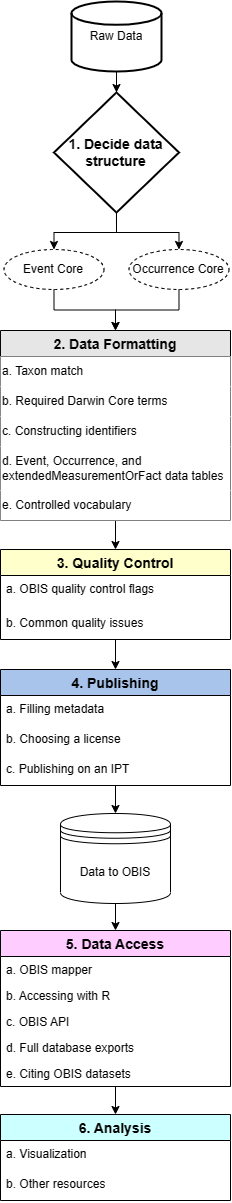
\includegraphics{images/OBISdataLifeCycle.png}

}

\end{marginfigure}

The basic data life cycle for contributions to OBIS can be broken down
into six step-by-step phases:

\begin{enumerate}
\def\labelenumi{\arabic{enumi}.}
\tightlist
\item
  Data structure
\item
  Data formatting
\item
  Quality control
\item
  Publishing
\item
  Data access (downloading)
\item
  Data visualization
\end{enumerate}

Each of these phases are outlined in this manual and are composed of a
number of steps which are covered in the relevant sections.

After you have decided on your \href{formatting.html}{data structure}
and have moved to the Data Formatting stage, you must first
\href{name_matching.html}{match} the taxa in your dataset to a
registered list. In formatting your dataset you will ensure the
\href{checklist.html}{required OBIS terms} and
\href{identifiers.html}{identifiers} are mapped correctly to your data
fields and records.

Depending on your data structure, you will then format data into a
\href{data_format.html}{DwC-A} format with the appropriate Core table
(\href{format_event.html}{Event} or
\href{format_occurrence.html}{Occurrence}) with any applicable extension
tables. Any biotic or abiotic measurements will be moved into the
\href{format_emof.html}{extendedMeasurementOrFact table}. Before
proceeding to the \href{data_publication.html}{publishing} stage, there
are a number of \href{dataquality.html}{quality control} steps to
complete.

Once your data has been published, you and others can
\href{access.html}{access} datasets through various avenues and it
becomes part of OBIS' global database!

This may seem like a daunting process at first glance, but this manual
will walk you through each step, and the OBIS community is full of
\href{gethelp.html}{helpful resources}. Throughout the manual you will
find tutorials and tools to guide you from start to finish through the
OBIS data life cycle.

\hypertarget{who-is-responsible-for-each-phase}{%
\subsubsection{Who is responsible for each
phase?}\label{who-is-responsible-for-each-phase}}

Phases 1 through 3 are the responsibilities of the data provider, while
Phases 3 and 4 are shared between the data provider and the node
manager. Data users are involved in Phases 5 and 6.

The OBIS Secretariat is responsible for data processing and harvesting
published resources.

\hypertarget{biodiversity-data-standards}{%
\section{Biodiversity data
standards}\label{biodiversity-data-standards}}

From the very beginning, OBIS has championed the use of international
standards for biogeographic data. Without agreement on the application
of standards and protocols, OBIS would not have been able to build a
large central database. OBIS uses the following standards:

\begin{itemize}
\tightlist
\item
  \href{darwin_core.html}{Darwin Core}
\item
  \href{eml.html}{Ecological Metadata Language}
\item
  \href{data_format.html}{Darwin Core Archive and dataset structure}
\end{itemize}

The following pages of this manual review each of these in turn. We show
you how to apply these standards to format your data in the
\href{formatting.html}{Data Formatting} section.

We also provide some \href{examples.html}{dataset examples} for your
reference.

\hypertarget{darwin-core}{%
\subsection{Darwin Core}\label{darwin-core}}

\textbf{Contents}

\begin{itemize}
\tightlist
\item
  \protect\hyperlink{introduction-to-darwin-core}{Introduction to Darwin
  Core}
\item
  \protect\hyperlink{darwin-core-terms}{Darwin Core terms}\\
\item
  \protect\hyperlink{darwin-core-guidelines}{Darwin Core guidelines}

  \begin{itemize}
  \tightlist
  \item
    \protect\hyperlink{taxonomy-and-identification}{Taxonomy and
    identification}
  \item
    \protect\hyperlink{occurrence}{Occurrence}\\
  \item
    \protect\hyperlink{record-level-terms}{Record level terms}\\
  \item
    \protect\hyperlink{location}{Location}\\
  \item
    \protect\hyperlink{event}{Event}
  \item
    \protect\hyperlink{time}{Time}\\
  \item
    \protect\hyperlink{sampling}{Sampling}
  \end{itemize}
\end{itemize}

\hypertarget{introduction-to-darwin-core}{%
\subsubsection{Introduction to Darwin
Core}\label{introduction-to-darwin-core}}

\href{https://dwc.tdwg.org/}{Darwin Core} is a body of standards (i.e.,
identifiers, labels, definitions) that facilitate sharing biodiversity
informatics. It provides stable
\href{https://dwc.tdwg.org/terms/}{terms} and vocabularies related to
biological objects/data and their collection. Darwin Core is maintained
by \href{http://tdwg.org/}{TDWG (Biodiversity Information Standards,
formerly The International Working Group on Taxonomic Databases)}.
Stable terms and vocabularies are important for ensuring the datasets in
OBIS have consistently interpretable fields. By following Darwin Core
standards, both data providers and users can be certain of the
definition and quality of data.

\hypertarget{history-of-darwin-core-and-obis}{%
\paragraph{History of Darwin Core and
OBIS}\label{history-of-darwin-core-and-obis}}

The old \href{http://old.iobis.org/node/304}{OBIS schema} was an
\href{http://old.iobis.org/obis/obis.xsd}{OBIS extension} to Darwin Core
1.2., which was based on
\href{http://rs.tdwg.org/dwc/terms/simple/}{Simple Darwin Core}, a
subset of Darwin Core which does not allow any structure beyond rows and
columns. This old schema added some terms which were important for OBIS,
but were not supported by Darwin Core at the time (e.g., start and end
date and start and end latitude and longitude, depth range, lifestage,
and terms for abundance, biomass and sample size).

In 2009, the Executive Committee of TDWG announced their ratification of
an updated version of Darwin Core as a
\href{https://www.tdwg.org/community/dwc/\#history-and-context}{TDWG
Standard}. Ratified Darwin Core unifies specializations and innovations
emerging from diverse communities, and provides guidelines for ongoing
enhancement. The \href{https://dwc.tdwg.org/terms/}{Darwin Core Quick
Reference Guide} links to TDWG's term definitions and related practices
for Ratified Darwin Core. We will discuss the relevance of terms in this
guide further below.

In December 2013, the \href{https://obis.org/about/}{3rd session of the
IODE Steering Group for OBIS} agreed to transition OBIS globally to the
TDWG-Ratified version of Darwin Core, and the mapping of the (old) OBIS
specific terms to Darwin Core can be found
\href{http://rs.tdwg.org/dwc/terms/history/versions/index.htm\#dwcobis}{here}.

\hypertarget{darwin-core-dwc-terms}{%
\subsubsection{Darwin Core (DwC) terms}\label{darwin-core-dwc-terms}}

DwC terms correspond to the column names of your dataset and can be
grouped according to class type for convenience, e.g., Taxa, Occurrence,
Record, Location, etc. It is important to use DwC field names because
only columns using Darwin Core terms as headers will be recognized.

A list of all possible Darwin Core terms can be found on
\href{https://dwc.tdwg.org/terms/}{TDWG}. However, OBIS does not parse
all terms (note this doesn't mean you cannot include them, they just
will not be parsed when you publish to OBIS). Below is an overview of
the most relevant Darwin Core terms to consider when contributing to
OBIS, with guidelines regarding their use. We have also compiled a
convenient \href{checklist.html}{checklist} of OBIS-accepted terms,
their DwC class type, and which OBIS file (Event Core, Occurrence, eMoF,
etc.) it is likely to be found in.

Note that OBIS currently has seven required and one strongly recommended
DwC term: \texttt{occurrenceID}, \texttt{eventDate},
\texttt{decimalLongitude}, \texttt{decimalLatitude},
\texttt{scientificName}, \texttt{occurrenceStatus},
\texttt{basisOfRecord}, \texttt{scientificNameID} (strongly
recommended).

The following DwC terms are related to the Class \emph{Taxon}:

\begin{itemize}
\tightlist
\item
  scientificName
\item
  scientificNameID
\item
  scientificNameAuthorship
\item
  kingdom
\item
  taxonRank
\item
  taxonRemarks
\end{itemize}

The following DwC terms are related to the Class \emph{Identification}:

\begin{itemize}
\tightlist
\item
  identifiedBy
\item
  dateIdentified
\item
  identificationReferences
\item
  identificationRemarks
\item
  identificationQualifier
\item
  typeStatus
\end{itemize}

The following DwC terms are related to the Class \emph{Occurrence}:

\begin{itemize}
\tightlist
\item
  occurrenceID
\item
  occurrenceStatus
\item
  recordedBy
\item
  individualCount (OBIS recommends to add measurements to
  \protect\hyperlink{extendedmeasurementorfact-extension-emof}{eMoF})
\item
  organismQuantity (OBIS recommends to add measurements to
  \protect\hyperlink{extendedmeasurementorfact-extension-emof}{eMoF})
\item
  organismQuantityType (OBIS recommends to add measurements to
  \protect\hyperlink{extendedmeasurementorfact-extension-emof}{eMoF})
\item
  sex (OBIS recommends to add measurements to
  \protect\hyperlink{extendedmeasurementorfact-extension-emof}{eMoF})
\item
  lifeStage (OBIS recommends to add measurements to
  \protect\hyperlink{extendedmeasurementorfact-extension-emof}{eMoF})
\item
  behavior
\item
  associatedTaxa
\item
  occurrenceRemarks
\item
  associatedMedia
\item
  associatedReferences
\item
  associatedSequences
\item
  catalogNumber
\item
  preparations
\end{itemize}

The following DwC terms are related to the Class \emph{Record level}:

\begin{itemize}
\tightlist
\item
  basisOfRecord
\item
  institutionCode
\item
  collectionCode
\item
  collectionID
\item
  bibliographicCitation
\item
  modified
\item
  dataGeneralizations
\end{itemize}

The following DwC terms are related to the Class \emph{Location}:

\begin{itemize}
\tightlist
\item
  decimalLatitude
\item
  decimalLongitude
\item
  coordinateUncertaintyInMeters
\item
  geodeticDatum
\item
  footprintWKT
\item
  minimumDepthInMeters
\item
  maximumDepthInMeters
\item
  minimumDistanceAboveSurfaceInMeters
\item
  maximumDistanceAboveSurfaceInMeters
\item
  locality
\item
  waterBody
\item
  islandGroup
\item
  island
\item
  country
\item
  locationAccordingTo
\item
  locationRemarks
\item
  locationID
\end{itemize}

The following DwC terms are related to the Class \emph{Event}:

\begin{itemize}
\tightlist
\item
  parentEventID
\item
  eventID
\item
  eventDate
\item
  type
\item
  habitat
\item
  samplingProtocol (OBIS recommends to add sampling facts to
  \protect\hyperlink{extendedmeasurementorfact-extension-emof}{eMoF})
\item
  sampleSizeValue (OBIS recommends to add sampling facts to
  \protect\hyperlink{extendedmeasurementorfact-extension-emof}{eMoF})
\item
  SampleSizeUnit (OBIS recommends to add sampling facts to
  \protect\hyperlink{extendedmeasurementorfact-extension-emof}{eMoF})
\item
  samplingEffort (OBIS recommends to add sampling facts to
  \protect\hyperlink{extendedmeasurementorfact-extension-emof}{eMoF})
\end{itemize}

The following DwC terms are related to the Class \emph{MaterialSample}:

\begin{itemize}
\tightlist
\item
  materialSampleID
\end{itemize}

\hypertarget{darwin-core-guidelines}{%
\subsubsection{Darwin Core guidelines}\label{darwin-core-guidelines}}

\hypertarget{taxonomy-and-identification}{%
\paragraph{Taxonomy and
identification}\label{taxonomy-and-identification}}

\texttt{scientificName} (required term) should always contain the
originally recorded scientific name, even if the name is currently a
synonym. This is necessary to be able to track back records to the
original dataset. The name should be at the lowest possible taxonomic
rank, preferably at species level or lower, but higher ranks, such as
genus, family, order, class etc. are also acceptable. We recommend to
not include authorship in \texttt{scientificName}, and only use
\texttt{scientificNameAuthorship} for that purpose. The
\texttt{scientificName} term should only contain the name and not
identification qualifications (such as ?, confer or affinity), which
should instead be supplied in the \texttt{IdentificationQualifier} term,
see examples below. \texttt{taxonRemarks} can capture comments or notes
about the taxon or name.

A \href{http://www.marinespecies.org/}{WoRMS} LSID should be added in
\texttt{scientificNameID} (strongly recommended term), OBIS will use
this identifier to pull the taxonomic information from the World
Register of Marine Species (WoRMS) into OBIS and attach it to your
dataset. This information includes:

\begin{itemize}
\tightlist
\item
  Taxonomic classification (kingdom through species)
\item
  The accepted name in case of invalid names or synonyms
\item
  AphiaID
\item
  IUCN red list category
\end{itemize}

LSIDs are persistent, location-independent, resource identifiers for
uniquely naming biologically significant resources. More information on
LSIDs can be found at \href{http://www.lsid.info/}{www.lsid.info}. For
example, the WoRMS LSID for \emph{Solea solea} is:
urn:lsid:marinespecies.org:taxname:127160, and can be found at the
bottom of each WoRMS taxon page,
e.g.~\href{http://marinespecies.org/aphia.php?p=taxdetails\&id=127160}{\emph{Solea
solea}}.

\texttt{kingdom} and \texttt{taxonRank} can help us in identifying the
provided \texttt{scientificName} in case the name is not available in
WoRMS. \texttt{kingdom} in particular can help us find alternative
genus-species combinations and avoids linking the name to homonyms.
Please contact the WoRMS data management team (info@marinespecies.org)
in case the scientificName is missing in WoRMS. \texttt{kingdom} and
\texttt{taxonRank} are not necessary when a correct
\texttt{scientificNameID} is provided.

OBIS recommends providing information about how an identification was
made, for example by which ID key, species guide or expert; and by which
method (e.g morphology vs.~genomics), etc. The person's name who made
the taxonomic identification can go in \texttt{identifiedBy} and
\emph{when} in \texttt{dateIdentified}. Use the ISO 8601:2004(E)
standard for date and time, for instructions see
\protect\hyperlink{time}{Time}. A list of references, such as field
guides used for the identification can be listed in
\texttt{identificationReferences}. Any other information, such as
identification methods, can be added to \texttt{identificationRemarks}.

Examples:

\begin{longtable}[]{@{}
  >{\raggedright\arraybackslash}p{(\columnwidth - 8\tabcolsep) * \real{0.4388}}
  >{\raggedright\arraybackslash}p{(\columnwidth - 8\tabcolsep) * \real{0.2347}}
  >{\raggedright\arraybackslash}p{(\columnwidth - 8\tabcolsep) * \real{0.1020}}
  >{\raggedright\arraybackslash}p{(\columnwidth - 8\tabcolsep) * \real{0.1020}}
  >{\raggedright\arraybackslash}p{(\columnwidth - 8\tabcolsep) * \real{0.1224}}@{}}
\toprule\noalign{}
\begin{minipage}[b]{\linewidth}\raggedright
scientificNameID
\end{minipage} & \begin{minipage}[b]{\linewidth}\raggedright
scientificName
\end{minipage} & \begin{minipage}[b]{\linewidth}\raggedright
kingdom
\end{minipage} & \begin{minipage}[b]{\linewidth}\raggedright
phylum
\end{minipage} & \begin{minipage}[b]{\linewidth}\raggedright
class
\end{minipage} \\
\midrule\noalign{}
\endhead
\bottomrule\noalign{}
\endlastfoot
urn:lsid:marinespecies.org:taxname:142004 & Yoldiella nana & Animalia &
Mollusca & Bivalvia \\
urn:lsid:marinespecies.org:taxname:140584 & Ennucula tenuis & Animalia &
Mollusca & Bivalvia \\
urn:lsid:marinespecies.org:taxname:131573 & Terebellides stroemii &
Animalia & Annelida & Polychaeta \\
\end{longtable}

\begin{longtable}[]{@{}
  >{\raggedright\arraybackslash}p{(\columnwidth - 8\tabcolsep) * \real{0.1477}}
  >{\raggedright\arraybackslash}p{(\columnwidth - 8\tabcolsep) * \real{0.2045}}
  >{\raggedright\arraybackslash}p{(\columnwidth - 8\tabcolsep) * \real{0.1591}}
  >{\raggedright\arraybackslash}p{(\columnwidth - 8\tabcolsep) * \real{0.1932}}
  >{\raggedright\arraybackslash}p{(\columnwidth - 8\tabcolsep) * \real{0.2955}}@{}}
\toprule\noalign{}
\begin{minipage}[b]{\linewidth}\raggedright
order
\end{minipage} & \begin{minipage}[b]{\linewidth}\raggedright
family
\end{minipage} & \begin{minipage}[b]{\linewidth}\raggedright
genus
\end{minipage} & \begin{minipage}[b]{\linewidth}\raggedright
specificEpithet
\end{minipage} & \begin{minipage}[b]{\linewidth}\raggedright
scientificNameAuthorship
\end{minipage} \\
\midrule\noalign{}
\endhead
\bottomrule\noalign{}
\endlastfoot
Nuculanoida & Yoldiidae & Yoldiella & nana & (Sars M., 1865) \\
Nuculoida & Nuculidae & Ennucula & tenuis & (Montagu, 1808) \\
Terebellida & Trichobranchidae & Terebellides & stroemii & Sars, 1835 \\
\end{longtable}

\emph{Data from
\href{http://ipt.vliz.be/eurobis/resource?r=largenet_k2}{Benthic fauna
around Franz Josef Land}.}

If the record represents a nomenclatural type specimen, the term
\texttt{typeStatus} can be used, e.g.~for holotype, syntype, etc.

\textbf{In case of low confidence identifications}, and the scientific
name contains qualifiers such as \emph{cf.}, \emph{?} or \emph{aff.},
then this name should go in \texttt{identificationQualifier}, and
\texttt{scientificName} should contain the name of the lowest possible
taxon rank that refers to the most accurate identification. E.g. if the
specimen was accurately identified down to genus level, but not species
level, then the scientificName should contain the name of the genus, the
scientificNameID should contain the LSID the genus and the
\texttt{identificationQualifier} should contain the low confidence
species name combined with \emph{?} or other qualifiers. The table below
shows a few examples:

The use and definitions for additional ON signs
(\texttt{identificationQualifier}) can be found in
\href{https://doi.org/10.1111/2041-210X.12594}{Open Nomenclature in the
biodiversity era}, which provides examples for using the main Open
Nomenclature qualifiers associated with \emph{physical specimens}. The
publication
\href{https://www.frontiersin.org/articles/10.3389/fmars.2021.620702/full}{Recommendations
for the Standardisation of Open Taxonomic Nomenclature for Image-Based
Identifications} provides examples and definitions for
\texttt{identificationQualifiers} for \emph{non-physical specimens
(image-based)}.

Examples:

\begin{longtable}[]{@{}
  >{\raggedright\arraybackslash}p{(\columnwidth - 10\tabcolsep) * \real{0.1173}}
  >{\raggedright\arraybackslash}p{(\columnwidth - 10\tabcolsep) * \real{0.2291}}
  >{\raggedright\arraybackslash}p{(\columnwidth - 10\tabcolsep) * \real{0.2402}}
  >{\raggedright\arraybackslash}p{(\columnwidth - 10\tabcolsep) * \real{0.0615}}
  >{\raggedright\arraybackslash}p{(\columnwidth - 10\tabcolsep) * \real{0.1453}}
  >{\raggedright\arraybackslash}p{(\columnwidth - 10\tabcolsep) * \real{0.2067}}@{}}
\toprule\noalign{}
\begin{minipage}[b]{\linewidth}\raggedright
scientificName
\end{minipage} & \begin{minipage}[b]{\linewidth}\raggedright
scientificNameAuthorship
\end{minipage} & \begin{minipage}[b]{\linewidth}\raggedright
scientificNameID
\end{minipage} & \begin{minipage}[b]{\linewidth}\raggedright
taxonRank
\end{minipage} & \begin{minipage}[b]{\linewidth}\raggedright
identificationQualifier
\end{minipage} & \begin{minipage}[b]{\linewidth}\raggedright
taxonConceptID
\end{minipage} \\
\midrule\noalign{}
\endhead
\bottomrule\noalign{}
\endlastfoot
Pelagia & Péron \& Lesueur, 1810 &
urn:lsid:marinespecies.org:taxname:135262 & genus & gen. nov. & Pelagia
gen. nov. \\
Pelagia benovici & Piraino, Aglieri, Scorrano \& Boero, 2014 &
urn:lsid:marinespecies.org:taxname:851656 & species & sp. nov & Pelagia
benovici sp. nov \\
Gadus & Linnaeus, 1758 & urn:lsid:marinespecies.org:taxname:125732 &
genus & cf.~morhua & Gadus cf.~morhua \\
Polycera & Cuvier, 1816 & urn:lsid:marinespecies.org:taxname:138369 &
genus & cf.~hedgpethi & Polycera cf.~hedgpethi \\
Tubifex & Lamarck, 1816 & urn:lsid:marinespecies.org:taxname:137392 &
genus & ? & Tubifex tubifex(Müller, 1774)? \\
Tubifex & Lamarck, 1816 & urn:lsid:marinespecies.org:taxname:137392 &
genus & sp. inc. & Tubifex tubifex(Müller, 1774)sp. inc. \\
Brisinga & Asbjørnsen, 1856 & urn:lsid:marinespecies.org:taxname:123210
& genus & gen. inc. & Brisinga gen. inc. \\
Uroptychus compressus & Baba \& Wicksten, 2019 &
urn:lsid:marinespecies.org:taxname:1332465 & genus & sp. inc. &
Uroptychus compressus sp. inc. \\
Eurythenes & S. I. Smith in Scudder, 1882 &
urn:lsid:marinespecies.org:taxname:101607 & genus & sp.
DISCOLL.PAP.JC165.674 & Eurythenes sp.DISCOLL.PAP.JC165.674 \\
Paroriza & Hérouard, 1902 & urn:lsid:marinespecies.org:taxname:123467 &
genus & sp.{[}unique123{]}aff.pallens & Paroriza sp.{[}unique123{]}aff.
pallens \\
Aristeidae & Wood-Mason in Wood-Mason \& Alcock, 1891 &
urn:lsid:marinespecies.org:taxname:106725 & family & stet. & Aristeidae
stet. \\
Nematocarcinus & Milne-Edwards, 1881 &
urn:lsid:marinespecies.org:taxname:107015 & genus & sp.indet. &
Nematocarcinus sp.indet. \\
Brisinga & Asbjørnsen, 1856 & urn:lsid:marinespecies.org:taxname:123210
& genus & gen.inc. & Brisinga gen.inc. \\
Brisinga costata & Verrill, 1884 &
urn:lsid:marinespecies.org:taxname:17825 & species & sp.inc. & Brisinga
costata sp.inc. \\
\end{longtable}

\hypertarget{occurrence}{%
\paragraph{Occurrence}\label{occurrence}}

\texttt{occurrenceID} (required term) is an identifier for the
occurrence record and should be persistent and globally unique. If the
dataset does not yet contain (globally unique) occurrenceIDs, then they
should be created. Guideline for ID creation can be found
\href{identifiers.html}{here}

\texttt{occurrenceStatus} (required term) is a statement about the
presence or absence of a taxon at a location. It is an important term,
because it allows us to distinguish between presence and absence
records. It is a required term and should be filled in with either
\texttt{present} or \texttt{absent}.

A few terms related to quantity: \texttt{organismQuantity} and
\texttt{organismQuantityType}, have been added to the TDWG ratified
Darwin Core. This is a lot more versatile than the older
\texttt{individualCount} field. However, OBIS recommends to use the
\protect\hyperlink{extendedmeasurementorfact-extension-emof}{Extended
MeasurementorFact extension} for quantitative measurements because of
the standardization of terms and the fact that you can link these
measurements to sampling events and factual sampling information.

Please take note that OBIS recommends all quantitative measurements and
sampling facts to be placed in the \texttt{ExtendedMeasurementOrFact}
extension and not in the Darwin Core files.

In the case specimens were collected and stored (e.g.~museum
collections), the \texttt{catalogNumber} and \texttt{preparations} terms
can be used to provide the identifier for the record in the collection
and to document the preparation and preservation methods. The term
\texttt{typeStatus} see above (under identification) can be used in this
context too.

Both \texttt{associatedMedia}, \texttt{associatedReferences} and
\texttt{associatedSequences} are global unique identifiers or URIs
pointing to respectively associated media (e.g.~online image or video),
associated literature (e.g.~DOIs) or genetic sequence information
(e.g.~GenBANK ID).

\texttt{associatedTaxa} include a list (concatenated and separated) of
identifiers or names of taxa and their associations with the Occurrence,
e.g.~the species occurrence was associated to the presence of kelp such
as \emph{Laminaria digitata}.

The recommended vocabulary for \texttt{sex} see
\href{http://vocab.nerc.ac.uk/collection/S10/current/}{BODC vocab :
S10}, for \texttt{lifeStage} see
\href{http://vocab.nerc.ac.uk/collection/S11/current/}{BODC vocab: S11},
\texttt{behavior} (no vocab available), and \texttt{occurrenceRemarks}
can hold any comments or notes about the Occurrence.

\texttt{recordedBy} can hold a list (concatenated and separated) of
names of people, groups, or organizations responsible for recording the
original Occurrence. The primary collector or observer, especially one
who applies a personal identifier (recordNumber), should be listed
first.

Example:

\begin{longtable}[]{@{}
  >{\raggedright\arraybackslash}p{(\columnwidth - 6\tabcolsep) * \real{0.2419}}
  >{\raggedright\arraybackslash}p{(\columnwidth - 6\tabcolsep) * \real{0.3065}}
  >{\raggedright\arraybackslash}p{(\columnwidth - 6\tabcolsep) * \real{0.3065}}
  >{\raggedright\arraybackslash}p{(\columnwidth - 6\tabcolsep) * \real{0.1452}}@{}}
\toprule\noalign{}
\begin{minipage}[b]{\linewidth}\raggedright
collectionCode
\end{minipage} & \begin{minipage}[b]{\linewidth}\raggedright
occurrenceID
\end{minipage} & \begin{minipage}[b]{\linewidth}\raggedright
catalogNumber
\end{minipage} & \begin{minipage}[b]{\linewidth}\raggedright
occurrenceStatus
\end{minipage} \\
\midrule\noalign{}
\endhead
\bottomrule\noalign{}
\endlastfoot
SluiceDock\_benthic\_1976/1981 & SluiceDock\_benthic\_1976\_1 &
SluiceDock\_benthic\_1976\_1 & present \\
SluiceDock\_benthic\_1976/1981 & SluiceDock\_benthic\_1976\_2 &
SluiceDock\_benthic\_1976\_2 & present \\
SluiceDock\_benthic\_1976/1981 & SluiceDock\_benthic\_1979-07/1980-06\_1
& SluiceDock\_benthic\_1979-07/1980-06\_1 & present \\
\end{longtable}

\emph{Data from
\href{http://ipt.vliz.be/eurobis/resource?r=summary_of_benthic_studies_in_the_sluice_dock_ostend_during_1976-1981}{A
summary of benthic studies in the sluice dock of Ostend during
1976-1981}.}

\hypertarget{record-level-terms}{%
\paragraph{Record level terms}\label{record-level-terms}}

\texttt{basisOfRecord} (required term) specifies the nature of the
record, i.e.~whether the occurrence record is based on a stored specimen
or an observation. In case the specimen is collected and stored in a
collection (e.g.~at a museum, university, research institute), the
options are:

\begin{itemize}
\tightlist
\item
  \texttt{PreservedSpecimen} e.g.~preserved in ethanol, tissue etc.
\item
  \texttt{FossilSpecimen} a fossil, which allows OBIS to make the
  distinction between the date of collection and the time period the
  specimen was assumed alive
\item
  \texttt{LivingSpecimen} an intentionally kept/cultivated living
  specimen e.g.~in an aquarium or culture collection.
\end{itemize}

In case no specimen is deposited, the basis of record is either
\texttt{HumanObservation} (e.g bird sighting, benthic sample but
specimens were discarded after counting), or \texttt{MachineObservation}
(e.g.~for occurrences based on automated sensors such as image
recognition, etc). For records pertaining to genetic samples,
basisOfRecord can be \texttt{MaterialSample} (e.g.~in the DNA-derived
data extension).

When the basisOfRecord is either a \emph{preservedSpecimen},
\emph{LivingSpecimen} or \emph{FossilSpecimen} please also add the
\texttt{institutionCode}, \texttt{collectionCode} and
\texttt{catalogNumber}, which will enable people to visit the collection
and re-examine the material. Sometimes, for example in case of living
specimens, a dataset can contain records pointing to the origin, the
in-situ sampling position as well as a record referring to the ex-situ
collection. In this case please add the event type information in
\texttt{eventRemarks} (see \protect\hyperlink{event}{OBIS manual:
event}).

\texttt{institutionCode} identifies the custodian institute (often by
acronym), \texttt{collectionCode} identifies the collection or dataset
within that institute. Collections cannot belong to multiple institutes,
so all records within a collection should have the same
\texttt{institutionCode}. The \texttt{collectionID} is an identifier for
the record within the dataset or collection.

\texttt{bibliographicCitation} allows for providing different citations
on record level, while a single citation for the entire dataset can and
should be provided in the metadata (see \href{eml.html}{EML}). The
citation at record level can have the format of a chapter in a book,
where the book is the dataset citation. The record citation will have
preference over the dataset citation. We do not, however, recommend to
create different citations for every record, as this will explode the
number of citations and will hamper the re-use of data.

\texttt{modified} is the most recent date-time on which the resource was
changed. It is required to use the ISO 8601:2004(E) standard, for
instructions see \protect\hyperlink{time}{Time}.

\texttt{dataGeneralizations} refers to actions taken to make the shared
data less specific or complete than in its original form. Suggests that
alternative data of higher quality may be available on request. This can
be the case for occurrences of vulnerable or endangered species and
there positions are converted to the center of grid cells.

\hypertarget{location}{%
\paragraph{Location}\label{location}}

\texttt{decimalLatitude} and \texttt{decimalLongitude} (required terms)
are the geographic latitude and longitude (in decimal degrees), using
the spatial reference system given in \texttt{geodeticDatum} of the
geographic center of a Location. The number of decimals should be
appropriate for the level of uncertainty in
\texttt{coordinateUncertaintyInMeters} (at least within an order of
magnitude). \texttt{coordinateUncertaintyInMeters} is the radius of the
smallest circle around the given position containing the whole location.
Regarding \texttt{decimalLatitude}, positive values are north of the
Equator, negative values are south of it. All values lie between -90 and
90, inclusive. Regarding \texttt{decimalLongitude}, positive values are
east of the Greenwich Meridian, negative values are west of it. All
values lie between -180 and 180, inclusive.

In OBIS, the spatial reference system to be documented in
\texttt{geodeticDatum} is \href{https://epsg.io/4326}{EPSG:4326}.
Coordinates in degrees/minutes/seconds can be converted to decimal
degrees using our \href{http://iobis.github.io/coordinates/}{coordinates
tool}. We also provide a \href{https://obis.org/maptool}{tool} to check
coordinates or to determine coordinates for a location (point, transect
or polygon) on a map. This tool also allows geocoding location names
using \href{http://www.marineregions.org/}{marineregions.org}.

The name of the place or location can be provided in \texttt{locality},
and if possible linked by a \texttt{locationID} using a persistent ID
from a gazetter, such as the MRGID from
\href{http://www.marineregions.org/gazetteer.php?p=search}{MarineRegions}.
If the species occurrence only contains the name of the
\texttt{locality}, but not the exact coordinates, we recommend using a
geocoding service to obtain the coordinates.
\href{http://www.marineregions.org/}{Marine Regions} has a
\href{http://www.marineregions.org/gazetteer.php?p=search}{search
interface} for geographic names, and provides coordinates and often
precision in meters, which can go into
\texttt{coordinateUncertaintyInMeters}. Another option is to use the
\href{http://www.getty.edu/research/tools/vocabularies/tgn/}{Getty
Thesaurus of Geographic Names} or \href{http://maps.google.com}{Google
Maps}: after looking up a location, the decimal coordinates can be found
in the page URL. Additional information about the locality can also be
stored in DwC terms such as \texttt{waterBody}, \texttt{islandGroup},
\texttt{island} and \texttt{country}. \texttt{locationAccordingTo}
should provide the name of the gazetteer that is used to obtain the
coordinates for the locality.

\texttt{locationID} is an identifier for the set of location information
(e.g.~station ID, or MRGID from
\href{http://www.marineregion.org}{marineregions}), for example the
\href{http://www.marineregions.org/gazetteer.php?p=details\&id=3956}{Balearic
Plain} has MRGID: \url{http://marineregions.org/mrgid/3956}.

A \href{https://en.wikipedia.org/wiki/Well-known_text}{Well-Known Text}
(WKT) representation of the shape of the location can be provided in
\texttt{footprintWKT}. This is particularly useful for tracks,
transects, tows, trawls, habitat extent or when an exact location is not
known. WKT strings can be created using our
\href{https://obis.org/maptool}{WKT tool}. This tool also calculates a
midpoint and a radius, which can then be added to
\texttt{decimalLongitude}, \texttt{decimalLatitude}, and
\texttt{coordinateUncertaintyInMeters} respectively. There is also an
\href{https://github.com/iobis/obistools\#calculate-centroid-and-radius-for-wkt-geometries}{R
tool} to calculate the centroid and radius for WKT polygons.
\href{https://wktmap.com}{wktmap.com} can be used to visualize and share
WKT strings.

Some examples of WKT strings:

\begin{Shaded}
\begin{Highlighting}[]
\NormalTok{LINESTRING (30 10, 10 30, 40 40)}
\NormalTok{POLYGON ((30 10, 40 40, 20 40, 10 20, 30 10))}
\NormalTok{MULTILINESTRING ((10 10, 20 20, 10 40),(40 40, 30 30, 40 20, 30 10))}
\NormalTok{MULTIPOLYGON (((30 20, 45 40, 10 40, 30 20)),((15 5, 40 10, 10 20, 5 10, 15 5)))}
\end{Highlighting}
\end{Shaded}

Example:

\begin{longtable}[]{@{}
  >{\raggedright\arraybackslash}p{(\columnwidth - 10\tabcolsep) * \real{0.1269}}
  >{\raggedright\arraybackslash}p{(\columnwidth - 10\tabcolsep) * \real{0.1343}}
  >{\raggedright\arraybackslash}p{(\columnwidth - 10\tabcolsep) * \real{0.1119}}
  >{\raggedright\arraybackslash}p{(\columnwidth - 10\tabcolsep) * \real{0.2313}}
  >{\raggedright\arraybackslash}p{(\columnwidth - 10\tabcolsep) * \real{0.2910}}
  >{\raggedright\arraybackslash}p{(\columnwidth - 10\tabcolsep) * \real{0.1045}}@{}}
\toprule\noalign{}
\begin{minipage}[b]{\linewidth}\raggedright
decimalLatitude
\end{minipage} & \begin{minipage}[b]{\linewidth}\raggedright
decimalLongitude
\end{minipage} & \begin{minipage}[b]{\linewidth}\raggedright
geodeticDatum
\end{minipage} & \begin{minipage}[b]{\linewidth}\raggedright
coordinateUncertaintyInMeters
\end{minipage} & \begin{minipage}[b]{\linewidth}\raggedright
footprintWKT
\end{minipage} & \begin{minipage}[b]{\linewidth}\raggedright
footprintSRS
\end{minipage} \\
\midrule\noalign{}
\endhead
\bottomrule\noalign{}
\endlastfoot
38.698 & 20.95 & EPSG:4326 & 75033.17 & LINESTRING (20.31 39.15, 21.58
38.24) & EPSG:4326 \\
42.72 & 15.228 & EPSG:4326 & 154338.87 & LINESTRING (16.64 41.80, 13.82
43.64) & EPSG:4326 \\
39.292 & 20.364 & EPSG:4326 & 162083.27 & LINESTRING (19.05 40.34, 21.68
38.25) & EPSG:4326 \\
\end{longtable}

\emph{Data from
\href{http://ipt.vliz.be/eurobis/resource?r=ionian_2008_2018}{Adriatic
and Ionian Sea mega-fauna monitoring employing ferry as platform of
observation along the Ancona-Igoumenitsa-Patras lane, from December 2014
to December 2018}.}

Keep in mind while filling in
\href{http://rs.tdwg.org/dwc/terms/maximumDepthInMeters}{\texttt{minimumDepthInMeters}}
and
\href{http://rs.tdwg.org/dwc/terms/minimumDepthInMeters}{\texttt{maximumDepthInMeters}}
that this should be the depth at which the \textbf{sample was taken} and
not the water column depth at that location. When fillling in any depth
fields (\texttt{minimumDepthInMeters}, \texttt{maximumDepthInMeters},
\href{http://rs.tdwg.org/dwc/terms/minimumDistanceAboveSurfaceInMeters}{\texttt{minimumDistanceAboveSurfaceInMeters}},
and
\href{http://rs.tdwg.org/dwc/terms/maximumDistanceAboveSurfaceInMeters}{\texttt{maximumDistanceAboveSurfaceInMeters}}),
you should also consider which information is needed to fully understand
the data. In most cases (e.g.~scenario 1 and 4 in the figure below),
providing \texttt{minimumDepthInMeters} and
\texttt{maximumDepthInMeters} is sufficient for observations of
organisms at particular depths. However, in cases where an occurrence is
above the sea surface, e.g.~flying birds (scenario 2 and 5), you should
populate \texttt{minimumDistanceAboveSurfaceInMeters},
\texttt{maximumDistanceAboveSurfaceInMeters}, and, where relevant, you
should also include
\href{https://dwc.tdwg.org/list/\#dwc_minimumElevationInMeters}{\texttt{minimumElevationInMeters}}
and
\href{https://dwc.tdwg.org/list/\#dwc_maximumElevationInMeters}{\texttt{maximumElevationInMeters}}.

The \texttt{minimumDistanceAboveSurfaceInMeters} and
\texttt{maximumDistanceAboveSurfaceInMeters} is the distance, in meters,
above or below a reference surface or reference point. The reference
surface is determined by the depth or elevation. If the depth and
elevation are 0, then the reference surface is the sea surface. If a
depth is given, the reference surface is the location of the depth. This
can be especially useful for sediment cores taken from the sea bottom
(scenario 3 in figure below). If no depth is given, then the elevation
is the reference surface (scenario 5).

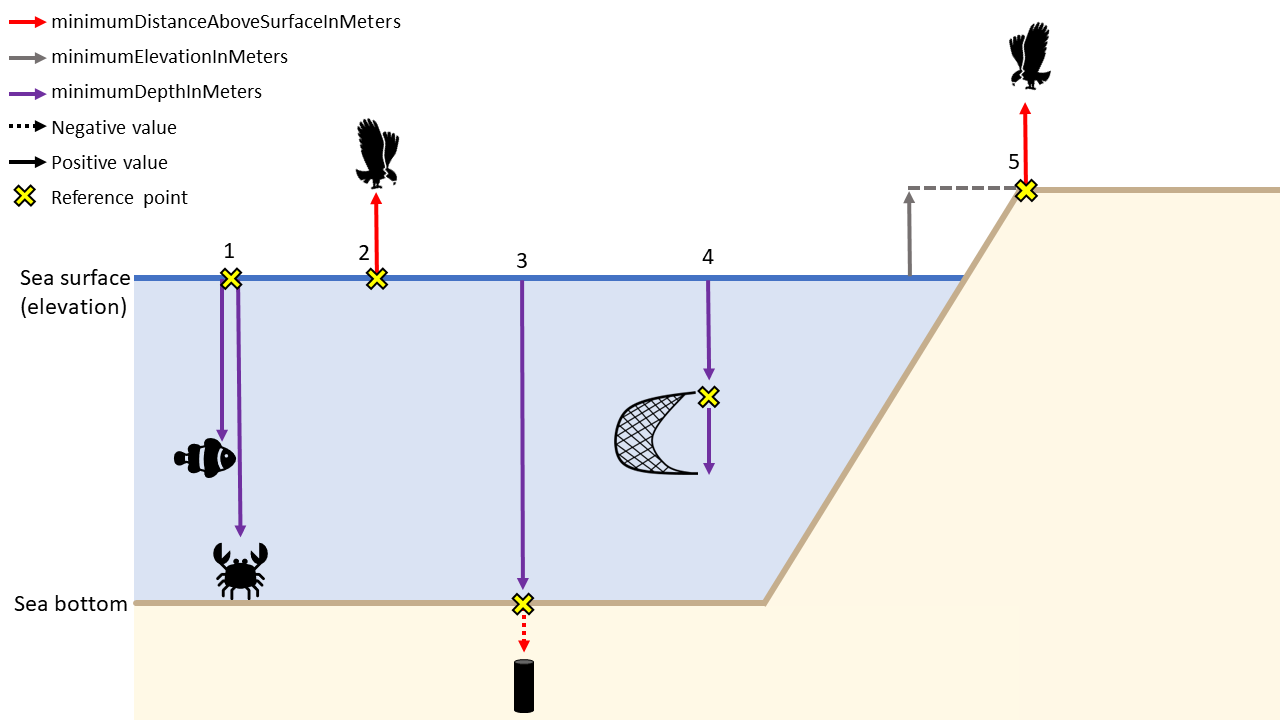
\includegraphics{images/Depth-figure-updated.png}

Depth scenario examples:

\begin{longtable}[]{@{}
  >{\raggedright\arraybackslash}p{(\columnwidth - 12\tabcolsep) * \real{0.0610}}
  >{\raggedright\arraybackslash}p{(\columnwidth - 12\tabcolsep) * \real{0.1341}}
  >{\raggedright\arraybackslash}p{(\columnwidth - 12\tabcolsep) * \real{0.1341}}
  >{\raggedright\arraybackslash}p{(\columnwidth - 12\tabcolsep) * \real{0.2256}}
  >{\raggedright\arraybackslash}p{(\columnwidth - 12\tabcolsep) * \real{0.2256}}
  >{\raggedright\arraybackslash}p{(\columnwidth - 12\tabcolsep) * \real{0.1098}}
  >{\raggedright\arraybackslash}p{(\columnwidth - 12\tabcolsep) * \real{0.1098}}@{}}
\toprule\noalign{}
\begin{minipage}[b]{\linewidth}\raggedright
Scenario
\end{minipage} & \begin{minipage}[b]{\linewidth}\raggedright
minimumDepthInMeters
\end{minipage} & \begin{minipage}[b]{\linewidth}\raggedright
maximumDepthInMeters
\end{minipage} & \begin{minipage}[b]{\linewidth}\raggedright
minimumDistanceAboveSurfaceInMeters
\end{minipage} & \begin{minipage}[b]{\linewidth}\raggedright
maximumDistanceAboveSurfaceInMeters
\end{minipage} & \begin{minipage}[b]{\linewidth}\raggedright
minimumElevationInMeters
\end{minipage} & \begin{minipage}[b]{\linewidth}\raggedright
maximumElevationInMeters
\end{minipage} \\
\midrule\noalign{}
\endhead
\bottomrule\noalign{}
\endlastfoot
1 & 40, 90 & 50, 100 & - & - & 0 & 0 \\
2 & 0 & 0 & 10 & 15 & 0 & 0 \\
3 & 100 & 100 & 0 & -1.5 & 0 & 0 \\
4 & 20 & 22 & - & - & 0 & 0 \\
5 & 0 & 0 & 10 & 15 & 10 & 10 \\
\end{longtable}

\hypertarget{event}{%
\paragraph{Event}\label{event}}

\texttt{eventID} is an identifier for the sampling or observation event.
\texttt{parentEventID} is an identifier for a parent event, which is
composed of one or more sub-sampling (child) events (eventIDs). See
\protect\hyperlink{eventid}{identifiers} for details on how these terms
can be constructed.

\texttt{habitat} is a category or description of the habitat in which
the Event occurred (e.g.~benthos, seamount, hydrothermal vent, seagrass,
rocky shore, intertidal, ship wreck etc.)

\hypertarget{time}{%
\paragraph{Time}\label{time}}

The date and time at which an occurrence was recorded goes in
\texttt{eventDate}. This term uses the
\href{https://en.wikipedia.org/wiki/ISO_8601}{ISO 8601 standard} and
OBIS recommends using the extended ISO 8601 format with hyphens.

More specific guidelines on formatting dates and times can be found in
the \protect\hyperlink{temporal-dates-and-times}{Common Data formatting
issues page}

\hypertarget{sampling}{%
\paragraph{Sampling}\label{sampling}}

Information on \texttt{sampleSizeValue} and \texttt{sampleSizeUnit} is
very important when an organism quantity is specified. However, with
\href{data_format.html}{OBIS-ENV-DATA} it was felt that the extended
MeasurementorFact
(\href{http://rs.gbif.org/extension/obis/extended_measurement_or_fact.xml}{eMoF})
extension would be better suited than the DwC Event Core to store the
sampled area and/or volume because in some cases sampleSize by itself
may not be detailed enough to allow interpretation of the sample. For
instance, in the case of a plankton tow, the volume of water that passed
through the net is relevant. In case of Niskin bottles, the volume of
sieved water is more relevant than the actual volume in the bottle. In
these examples, as well as generally when recording sampling effort for
all protocols, eMoF enables greater flexibility to define parameters, as
well as the ability to describe the entire sample and treatment protocol
through multiple parameters. eMoF also allows you to standardize your
terms to a controlled vocabulary.

The next chapter deals with the metadata (description of the dataset) in
\href{eml.html}{Ecological Metadata Language}.

\hypertarget{darwin-core-archive}{%
\subsection{Darwin Core Archive}\label{darwin-core-archive}}

\textbf{Contents}

\begin{itemize}
\tightlist
\item
  \protect\hyperlink{darwin-core-archive}{Darwin Core Archive}
\item
  \protect\hyperlink{obis-holds-more-than-just-species-occurrences-the-env-data-approach}{OBIS
  holds more than just species occurrences: the ENV-DATA approach}

  \begin{itemize}
  \tightlist
  \item
    \protect\hyperlink{extendedmeasurementorfact-extension-emof}{ExtendedMeasurementOrFact
    Extension (eMoF)}
  \item
    \protect\hyperlink{edna-dna-derived-data-extension}{eDNA \& DNA
    derived data Extension}
  \item
    \protect\hyperlink{a-special-case-habitat-types}{A special case:
    habitat types}
  \end{itemize}
\item
  \protect\hyperlink{recommended-reading}{Recommended reading}
\end{itemize}

\hypertarget{darwin-core-archive-1}{%
\subsubsection{Darwin Core Archive}\label{darwin-core-archive-1}}

Darwin Core Archive (DwC-A) is the standard for packaging and publishing
biodiversity data using Darwin Core terms. It is the preferred format
for publishing data in OBIS and GBIF. The format is described in the
\href{https://dwc.tdwg.org/text/}{Darwin Core text guide}. A Darwin Core
Archive contains a number of text files, including data tables formatted
as CSV.

The conceptual data model of the Darwin Core Archive is a star schema
with a single core table, for example containing occurrence records or
event records, at the center of the star. Extension tables can
optionally be associated with the core table. It is not possible to link
extension tables to other extension tables (to form a so-called
snowflake schema). There is a one-to-many relationship between the core
and extension records, so each core record can have zero or more
extension records linked to it, and each extension record must be linked
to exactly one core record. Definitions for the core and extension
tables can be found \href{http://rs.gbif.org/}{here}.

Besides data tables, a Darwin Core Archive also contains two XML files:
one file which describes the archive and data file structure
(\texttt{meta.xml}), and one file which contains the dataset's metadata
(\texttt{eml.xml}).

Figure: structure of a Darwin Core Archive.

\hypertarget{obis-holds-more-than-just-species-occurrences-the-env-data-approach}{%
\subsubsection{OBIS holds more than just species occurrences: the
ENV-DATA
approach}\label{obis-holds-more-than-just-species-occurrences-the-env-data-approach}}

Data collected as part of marine biological research often include
measurements of habitat features (such as physical and chemical
parameters of the environment), biotic and biometric measurements (such
as body size, abundance, biomass), as wel as details regarding the
nature of the sampling or observation methods, equipment, and sampling
effort.

In the past, OBIS relied solely on the
\href{http://rs.gbif.org/core/dwc_occurrence_2015-07-02.xml}{Occurrence
Core}, and additional measurements were added in a structured format
(e.g.~JSON) in the Darwin Core term \texttt{dynamicProperties} inside
the occurrence records. This approach had significant downsides: the
format is difficult to construct and deconstruct, there is no
standardization of terms, and attributes which are shared by multiple
records (think sampling methodology) have to be repeated many times. The
formatting problem can be addressed by moving measurements to a
\href{http://rs.gbif.org/extension/dwc/measurements_or_facts.xml}{MeasurementOrFacts}
extension table, but that doesn't solve the redundancy and
standardization problems.

With the release and adoption of a new core type
\href{http://rs.gbif.org/core/dwc_event_2015_05_29.xml}{Event Core} it
became possible to associate measurements with nested events (such as
cruises, stations, and samples), but the restrictive star schema of
Darwin Core archive prohibited associating measurements with the event
records in the Event core as well as with the occurrence records in the
Occurrence extension. For this reason an extended version of the
existing MeasurementOrFact extension was created.

\hypertarget{extendedmeasurementorfact-extension-emof}{%
\paragraph{ExtendedMeasurementOrFact Extension
(eMoF)}\label{extendedmeasurementorfact-extension-emof}}

As part of the IODE pilot project
\href{https://www.iode.org/index.php?option=com_content\&view=article\&id=463\&Itemid=100200}{Expanding
OBIS with environmental data OBIS-ENV-DATA}, OBIS introduced a custom
\href{http://rs.gbif.org/extension/obis/extended_measurement_or_fact.xml}{ExtendedMeasurementOrFact}
or eMoF extension, which extends the existing
\href{http://rs.gbif.org/extension/dwc/measurements_or_facts.xml}{MeasurementOrFact}
extension with 4 new terms:

\begin{itemize}
\tightlist
\item
  \texttt{occurrenceID}
\item
  \texttt{measurementTypeID}
\item
  \texttt{measurementValueID}
\item
  \texttt{measurementUnitID}
\end{itemize}

The \texttt{occurrenceID} term is used to circumvent the limitations of
the star schema, and link measurement records in the
ExtendedMeasurementOrFact extension to occurrence records in the
Occurrence extension. Note that in order to comply with the Darwin Core
Archive standard, these records still need to link to an event record in
the Event core table as well. Thanks to this term we can now store a
variety of measurements and facts linked to either events or
occurrences:

\begin{itemize}
\tightlist
\item
  organism quantifications (e.g.~counts, abundance, biomass, \% live
  cover, etc.)
\item
  species biometrics (e.g.~body length, weight, etc.)
\item
  facts documenting a specimen (e.g.~living/dead, behaviour,
  invasiveness, etc.)
\item
  abiotic measurements (e.g.~temperature, salinity, oxygen, sediment
  grain size, habitat features)
\item
  facts documenting the sampling activity (e.g.~sampling device, sampled
  area, sampled volume, sieve mesh size).
\end{itemize}

Figure: Overview of an OBIS-ENV-DATA format. Sampling parameters,
abiotic measurements, and occurrences are linked to events using the
eventID (full lines). Biotic measurements are linked to occurrences
using the new occurrenceID field of the ExtendedMeasurementOrFact
Extension (dashed lines).

\hypertarget{edna-dna-derived-data-extension}{%
\paragraph{eDNA \& DNA derived data
Extension}\label{edna-dna-derived-data-extension}}

DNA derived data are increasingly being used to document taxon
occurrences. To ensure these data are useful to the broadest possible
community, GBIF published a guide entitled
\href{https://docs.gbif-uat.org/publishing-dna-derived-data/1.0/en/}{Publishing
DNA-derived data through biodiversity data platforms}. This guide is
supported by the DNA derived data extension for Darwin Core, which
incorporates MIxS terms into the Darwin Core standard. eDNA and DNA
derived data is linked to occurrence data with the use of
\texttt{occurrenceID} and/ or \texttt{eventID}. Refer to the
\href{dna_data.html}{Examples: ENV-DATA and DNA derived data} for use
case examples of eDNA and DNA derived data.

\hypertarget{a-special-case-habitat-types}{%
\paragraph{A special case: habitat
types}\label{a-special-case-habitat-types}}

Including information on habitats (biological community, biotope, or
habitat type) is possible and encouraged with the use of Event Core.
However, beware the unconstrained nature of the terms
\texttt{measurementTypeID}, \texttt{measurementValueID}, and
\texttt{measurementUnitID} which can lead to inconsistently documented
habitat measurements within the Darwin Core Archive standard. To ensure
this data is more easily discoverable, understood or usable, refer to
\protect\hyperlink{habitat-data}{Examples: habitat data} and/or
\href{https://emodnet.ec.europa.eu/en/reports?field_emodnet_lot_value\%5B\%5D=seabed_habitats\#h3298bcd0a15741a8a0ac1c8b4576f7c5}{Duncan
et al.~(2021)} for use case examples and more details.

\hypertarget{recommended-reading}{%
\paragraph{Recommended reading}\label{recommended-reading}}

\begin{itemize}
\tightlist
\item
  \href{https://bdj.pensoft.net/articles.php?id=10989}{De Pooter et
  al.~2017}. Toward a new data standard for combined marine biological
  and environmental datasets - expanding OBIS beyond species
  occurrences. Biodiversity Data Journal 5: e10989.
  hdl.handle.net/10.3897/BDJ.5.e10989
\item
  \href{https://emodnet.ec.europa.eu/en/reports?field_emodnet_lot_value\%5B\%5D=seabed_habitats\#h3298bcd0a15741a8a0ac1c8b4576f7c5}{Duncan
  et al.~(2021)}. A standard approach to structuring classified habitat
  data using the Darwin Core Extended Measurement or Fact Extension.
  EMODnet report. \emph{(Note you must refine search to Technical
  Reports from 2021 to identify Duncan et al.'s report)}
\end{itemize}

\hypertarget{relational-databases-the-underlying-framework-of-obis}{%
\subsection{Relational databases: the underlying framework of
OBIS}\label{relational-databases-the-underlying-framework-of-obis}}

If you are not familiar with relational databases, it can be difficult
to understand the underlying framework OBIS relies on. This section will
help you understand relational databases, how they relate to OBIS, the
data you will format for OBIS, and the data you may download from OBIS.

Why do we use relational databases in the first place? You are probably
familiar with flat databases which contain all data in one table - this
is likely how your own data are formatted. Relational databases instead
consist of multiple data tables that each contain \emph{related}
information. When all this information is presented in one table, the
table becomes larger, very complicated, and the likelihood of data
duplication increases. Relational databases seek to simplify
complexities and \protect\hyperlink{how-to-avoid-redundancy}{reduce
redundancy} by allowing information to be self-contained, but linked to
each other.

You can think of a relational database as separate Excel sheets or data
tables that are related to each other. One data table could be a
``core'' table, whereas others are ``extensions''. Sometimes the
relationships between core and extension tables are hierarchical, but
this is not always the case. There is, however, always a
\emph{relationship} linking core and extension tables.

Let's review core and extension tables and how we use them for OBIS.

Core tables contain information that is applicable to \textbf{all}
extension tables, and extension tables contain more information about
the records within the Core table. Each table, whether core or
extension, contains records and attributes. Each row is a record (e.g.,
a sampling event, a species' occurrence), whereas each column is an
attribute (e.g., a date, a measurement).

Records between tables are linked to each other by the use of
\emph{identifiers}. A description of measurements pertaining to a record
in an Extension table will have the same identifier as the record it is
describing in the Core table. By using identifiers to link records, we
reduce data repetition, see
\protect\hyperlink{how-to-avoid-redundancy}{below} for examples. In the
Darwin Core format that OBIS uses, the core table is either
\href{https://manual.obis.org/data_format.html\#when-to-use-event-core}{Event}
or
\href{https://manual.obis.org/data_format.html\#when-to-use-occurrence-core}{Occurrence},
and datasets can have
\protect\hyperlink{extensions-accepted-by-OBIS}{one, none, or more}
extension tables. Further explanation of data formatting in OBIS is
covered in the \href{formatting.html}{Data Formatting section} of the
OBIS manual.

Let's review an example to fully understand how relational databases
work. We will look at a simple relational database used by a fictional
country that tracks student performance in three different courses
between three schools. Rather than trying to contain information about
each school, course, and student performance in one place, this
information is split into three separate tables. We see that the pink
table gives us information about each school - its name, and the
district it belongs to. Each school also has a schoolID, an identifier
linking to the blue table where we can see student performance (course
mean) in each course, the class size, and year. You will notice that the
course mean and class size are bundled under columns called
measurementType and measurementValue. These are similar to the eMoF
vocabularies and are integral to reducing repeated data, especially when
one dataset has reoccurring information. Finally we see that the
courseID in the blue table links to the yellow one with the courseID
identifier, giving us information about each course.

A fourth table could easily be created to track total school population
size through time. In contrast, if this information was only presented
in the pink Schools in Country table, the school information would be
duplicated as you add rows for each year. In this way, you can easily
see how useful relational databases are. Of course, this is a simplified
example but it demonstrates how related tables can be linked by
identifiers to reduce table complexity and data replication.

We elaborate on how this structure is applied within OBIS
\protect\hyperlink{dataset-structure}{here}.

\begin{figure}

{\centering 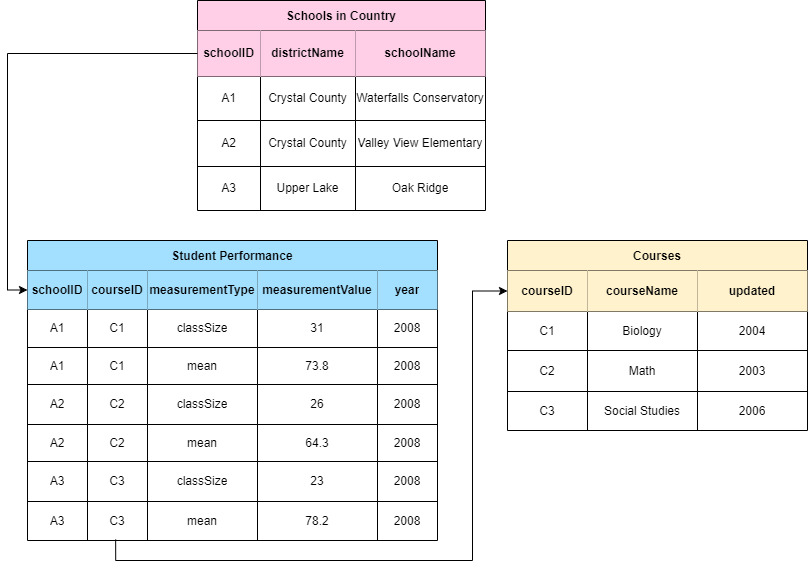
\includegraphics[width=0.8\textwidth,height=\textheight]{images/relationalDB-updated.png}

}

\caption{\emph{An example of how a relational database works. Three
tables show the (1) student performance (blue table) in (2) different
schools (pink table) in a fictional country, and (3) the names of the
courses (yellow table). Information between each table is linked by the
use of identifiers, indicated by the arrows}}

\end{figure}

Note that when OBIS harvests data, datasets are flattened - i.e., all
separate data tables are combined into one. This is the kind of file you
will receive when you \href{access.html}{download data from OBIS}. The
reason for this is that querying relational databases significantly
reduces computational time, as opposed to querying a flat database.
Relational databases also facilitate requests for subsets that meet
particular criteria - e.g., all data from Norway for one species above a
certain depth.

\hypertarget{how-to-avoid-redundancy}{%
\subsubsection{How to avoid redundancy}\label{how-to-avoid-redundancy}}

Avoiding redundancy and data duplication within your dataset is built
into the OBIS data structure. Utilizing the ENV-DATA approach, which
delineates relationships between the core table and extension tables, we
can limit the repetition of data.

For example, let us consider the dates of a ship cruise where a series
of bottom trawls were taken. The sampling information (e.g., date range,
equipment used, etc.) for each species collected in these trawls is the
same. Because of this, we know we are dealing with unique sampling
events and thus we will use \href{format_event.html}{Event core}. So,
our Event core table will contain all information related to the
sampling events (e.g., date, location). Then, information pertaining to
each collected species (e.g., abundance, biomass, sampling methods,
etc.) will be placed in an extension, the (Extended)MeasurementOrFact
table. Here, each measurement for each species and sample will occur on
a separate record. These records will be linked to the correct sampling
event in the Event core by an identifier - the eventID. If we were to
put this data in one file, the fields related to date and location
(e.g., eventDate, decimalLongitude, decimalLatitude, etc.) would be
repeated for each species.

Let's consider another example. If you took one temperature measurement
from the water column where you took your sample, each species found in
that sample would have the \textbf{same} temperature measurement. By
linking such measurements to the \emph{event} instead of each
\emph{occurrence}, we are able to reduce the amount of data being
repeated.

\begin{figure}

{\centering 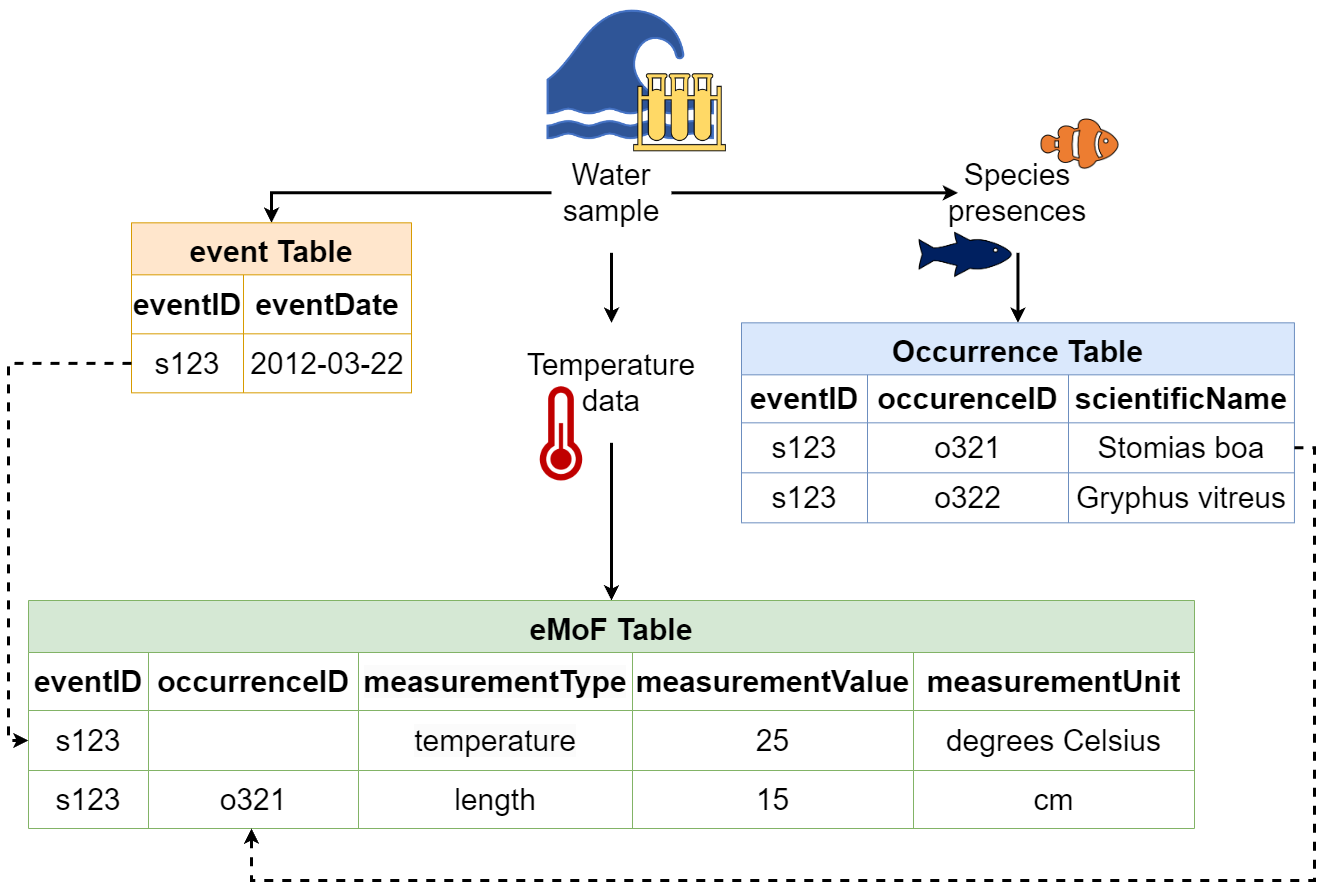
\includegraphics[width=0.8\textwidth,height=\textheight]{images/OBIS-sampling-schema-example-update.png}

}

\caption{\emph{Example of how the sample data is distributed to Core and
Extension tables, and how these tables are connected in OBIS}}

\end{figure}

An advantage of structuring data this way is that if any mistakes are
made, you only need to correct it once! So you can see that using
relational event structures (when applicable) in combination with
extension files can really simplify and reduce the number of times data
are repeated.

\textbf{Caveat:} However we would like to note that in some cases, data
duplication may occur due to the star schema structure. For example,
when publishing DNA-derived data,
\href{https://docs.gbif.org/publishing-dna-derived-data/1.0/en/\#data-packaging-and-mapping}{Occurrence
core will have to be used}, which necessitates the repetition of event
data for each occurrence record.

\hypertarget{ecological-metadata-language}{%
\subsection{Ecological Metadata
Language}\label{ecological-metadata-language}}

OBIS (and GBIF) uses the Ecological Metadata Language (EML) as its
metadata standard, which is specifically developed for the earth,
environmental and ecological sciences. It is based on prior work done by
the Ecological Society of America and associated efforts. EML is
implemented as XML. See more information on
\href{https://eml.ecoinformatics.org/}{EML}.

OBIS uses the
\href{http://rs.gbif.org/schema/eml-gbif-profile/1.1/eml-gbif-profile.xsd}{GBIF
EML profile (version 1.1)}. In case data providers use
ISO19115/ISO19139, there is a mapping available
\href{http://rs.gbif.org/schema/eml-gbif-profile/1.1/eml2iso19139.xsl}{here}.

For OBIS, the following 4 terms are the bare minimum required:
\texttt{Title}, \texttt{Citation}, \texttt{Contact} and
\texttt{Abstract}. Below is an overview of all the EML terms used to
describe datasets:

\begin{itemize}
\item
  \texttt{title\ {[}xml:lang="..."{]}}: A good descriptive
  \texttt{title} is indispensable and can provide the user with valuable
  information, making the discovery of data easier. Multiple titles may
  be provided, particularly when trying to express the title in more
  than one language (use the ``xml:lang'' attribute to indicate the
  language if not English/en).
\item
  \texttt{creator} ; \texttt{metadataProvider} ;
  \texttt{associatedParty} ; \texttt{contact} : These are the people and
  organizations responsible for the dataset resource, either as the
  creator, the metadata provider, contact person or any other
  association. The following details can be provided:

  \begin{itemize}
  \tightlist
  \item
    \texttt{individualName}

    \begin{itemize}
    \tightlist
    \item
      \texttt{givenName}
    \item
      \texttt{surName}
    \end{itemize}
  \item
    \texttt{organizationName}: Name of the institution.
  \item
    \texttt{positionName}: to be used as alternative to persons names
    (leave \texttt{individualName} blank and use \texttt{positionName}
    instead e.g.~data manager).
  \item
    \texttt{address}

    \begin{itemize}
    \tightlist
    \item
      \texttt{deliveryPoint}
    \item
      \texttt{city}
    \item
      \texttt{administrativeArea}
    \item
      \texttt{postalCode}
    \item
      \texttt{country}
    \end{itemize}
  \item
    \texttt{phone}\strut \\
  \item
    \texttt{electronicMailAddress}
  \item
    \texttt{onlineUrl} : personal website
  \item
    \texttt{role}: used with \texttt{associatedParty} to indicate the
    role of the associated person or organization.
  \item
    \texttt{userID}: e.g.~ORCID.

    \begin{itemize}
    \tightlist
    \item
      \texttt{directory}
    \end{itemize}
  \end{itemize}
\item
  \texttt{pubDate}: The date that the resource was published. Use ISO
  8601.
\item
  \texttt{language}: The language in which the resource (not the
  metadata document) is written. Use ISO language code.
\item
  \texttt{abstract} : Brief description of the data resource.

  \begin{itemize}
  \tightlist
  \item
    \texttt{para}
  \end{itemize}
\item
  \texttt{keywordSet}

  \begin{itemize}
  \tightlist
  \item
    \texttt{keyword} : Note only one keyword per keyword field is
    allowed.
  \item
    \texttt{keywordThesaurus} : e.g.~ASFA
  \end{itemize}
\item
  \texttt{additionalInfo} : OBIS checks this EML field for harvesting.
  It should contain \emph{marine, harvested by iOBIS}.

  \begin{itemize}
  \tightlist
  \item
    \texttt{para}
  \end{itemize}
\item
  \texttt{coverage}

  \begin{itemize}
  \tightlist
  \item
    \texttt{geographicCoverage}

    \begin{itemize}
    \tightlist
    \item
      \texttt{geographicDescription}: a short text description of the
      area. E.g. the river mounth of the Scheldt Estuary.
    \item
      \texttt{boundingCoordinates}

      \begin{itemize}
      \tightlist
      \item
        \texttt{westBoundingCoordinate}
      \item
        \texttt{eastBoundingCoordinate}
      \item
        \texttt{northBoundingCoordinate}
      \item
        \texttt{southBoundingCoordinate}
      \end{itemize}
    \end{itemize}
  \item
    \texttt{temporalCoverage} : Use ISO 8601

    \begin{itemize}
    \tightlist
    \item
      \texttt{singleDateTime}
    \item
      \texttt{rangeOfDates}

      \begin{itemize}
      \tightlist
      \item
        \texttt{beginDate}

        \begin{itemize}
        \tightlist
        \item
          \texttt{calendarDate}
        \end{itemize}
      \item
        \texttt{endDate}

        \begin{itemize}
        \tightlist
        \item
          \texttt{calendarDate}
        \end{itemize}
      \end{itemize}
    \end{itemize}
  \item
    \texttt{taxonomicCoverage}: taxonomic information about the dataset.
    It can include a species list.

    \begin{itemize}
    \tightlist
    \item
      \texttt{generalTaxonomicCoverage}
    \item
      \texttt{taxonomicClassification}

      \begin{itemize}
      \tightlist
      \item
        \texttt{taxonRankName}
      \item
        \texttt{taxonRankValue}
      \item
        \texttt{commonName}
      \end{itemize}
    \end{itemize}
  \end{itemize}
\item
  \texttt{intellectualRights}: Statement about IPR, Copyright or various
  Property Rights. Also read the \href{policy.html}{guidelines on the
  sharing and use of data in OBIS}.

  \begin{itemize}
  \tightlist
  \item
    \texttt{para}
  \end{itemize}
\item
  \texttt{purpose}: A description of the purpose of this dataset.

  \begin{itemize}
  \tightlist
  \item
    \texttt{para}
  \end{itemize}
\item
  \texttt{methods}

  \begin{itemize}
  \tightlist
  \item
    \texttt{methodStep}: Descriptions of procedures, relevant
    literature, software, instrumentation, source data and any quality
    control measures taken.
  \item
    \texttt{sampling}: Description of sampling procedures including the
    geographic, temporal and taxonomic coverage of the study.
  \item
    \texttt{studyExtent}: Description of the specific sampling area, the
    sampling frequency (temporal boundaries, frequency of occurrence),
    and groups of living organisms sampled (taxonomic coverage).
  \item
    \texttt{samplingDescription}: Description of sampling procedures,
    similar to the one found in the methods section of a journal
    article.

    \begin{itemize}
    \tightlist
    \item
      \texttt{para}
    \end{itemize}
  \item
    \texttt{qualityControl}: Description of actions taken to either
    control or assess the quality of data resulting from the associated
    method step.
  \end{itemize}
\item
  \texttt{project}

  \begin{itemize}
  \tightlist
  \item
    \texttt{title}
  \item
    \texttt{identifier}
  \item
    \texttt{personnel}: The personnel field is used to document people
    involved in a research project by providing contact information and
    their role in the project.
  \item
    \texttt{description}
  \item
    \texttt{funding}: The funding field is used to provide information
    about funding sources for the project such as: grant and contract
    numbers; names and addresses of funding sources.

    \begin{itemize}
    \tightlist
    \item
      \texttt{para}
    \end{itemize}
  \item
    \texttt{studyAreaDescription}
  \item
    \texttt{designDescription}: The description of research design.
  \end{itemize}
\item
  \texttt{maintenance}

  \begin{itemize}
  \tightlist
  \item
    \texttt{description}

    \begin{itemize}
    \tightlist
    \item
      \texttt{para}
    \end{itemize}
  \item
    \texttt{maintenanceUpdateFrequency}
  \end{itemize}
\item
  \texttt{additionalMetadata}

  \begin{itemize}
  \tightlist
  \item
    \texttt{metadata}

    \begin{itemize}
    \tightlist
    \item
      \texttt{dateStamp}: The dateTime the metadata document was created
      or modified (ISO 8601).
    \item
      \texttt{metadataLanguage}: The language in which the metadata
      document (as opposed to the resource being described by the
      metadata) is written
    \item
      \texttt{hierarchyLevel}

      \begin{itemize}
      \tightlist
      \item
        \texttt{citation} : A single citation for use when citing the
        dataset. The IPT can also auto-generate a citation based on the
        metadata (people, title, organization, onlineURL, DOI etc).
      \item
        \texttt{bibliography}: A list of citations that form a
        bibliography on literature related / used in the dataset
      \item
        \texttt{resourceLogoUrl}: URL of the logo associated with a
        dataset.
      \item
        \texttt{parentCollectionIdentifier}
      \item
        \texttt{collectionIdentifier}
      \item
        \texttt{formationPeriod}: Text description of the time period
        during which the collection was assembled. E.g., ``Victorian'',
        or ``1922 - 1932'', or ``c.~1750''.
      \item
        \texttt{livingTimePeriod}: Time period during which biological
        material was alive (for palaeontological collections).
      \item
        \texttt{specimenPreservationMethod}
      \item
        \texttt{physical}

        \begin{itemize}
        \tightlist
        \item
          \texttt{objectName}
        \item
          \texttt{characterEncoding}
        \item
          \texttt{dataFormat}

          \begin{itemize}
          \tightlist
          \item
            \texttt{externallyDefinedFormat}
          \item
            \texttt{formatName}
          \end{itemize}
        \item
          \texttt{distribution}: URL links

          \begin{itemize}
          \tightlist
          \item
            \texttt{online}

            \begin{itemize}
            \tightlist
            \item
              \texttt{url\ function="download"}
            \item
              \texttt{url\ function="information"}
            \end{itemize}
          \end{itemize}
        \end{itemize}
      \end{itemize}
    \end{itemize}
  \end{itemize}
\item
  \texttt{alternateIdentifier}: It is a Universally Unique Identifier
  (UUID) for the EML document and not for the dataset. This term is
  optional.
\end{itemize}

\hypertarget{metadata-sections}{%
\subsubsection{Metadata Sections}\label{metadata-sections}}

There are several categories/pages for metadata you must provide, which
includes basic information about the:

\begin{itemize}
\tightlist
\item
  Dataset and data provider
\item
  Geographic/taxonomic/temporal coverage
\item
  Keywords
\item
  Hosting institution information
\item
  Information regarding associated project(s)
\item
  Sampling methods
\item
  How to cite the dataset
\item
  Museum collection (if applicable)
\item
  Other external links (e.g.~a homepage) or additional metadata
\end{itemize}

We review each of these sections below.

\hypertarget{title}{%
\paragraph{Title}\label{title}}

The IPT requires you to provide a \emph{Shortname}. Shortnames serve as
an identifier for the resource within the IPT installation (so should be
unique within your IPT), and will be used as a parameter in the URL to
access the resource via the Internet. Please use only alphanumeric
characters, hyphens, or underscores. E.g. \emph{largenet\_im} in
\url{http://ipt.vliz.be/eurobis/resource?r=largenet_im}. After creating
a new dataset resource, the field title will be filled out with the
short name you provided earlier. Please make sure you provide a dataset
title following the guidelines below.

Dataset titles provided to OBIS node managers are often very cryptic,
such as an acronym, and often only understandable by the data provider.
However, to increase the discoverability and be useful for a larger
audience, the dataset title should be as descriptive and complete as
possible. OBIS recommends titles to contain information about the
taxonomic, geographic and temporal coverage. If the dataset title does
not meet these criteria and you believe the title should be changed,
then contact the data provider with a suggestion or ask for a more
descriptive title. If the dataset has already been published (made
publicly available) - and therefore known by that title elsewhere, then
the same title should be kept (even if it would not meet the proposed
guidelines)! Changing the title of an already published dataset cannot
be done, as this will generate confusion and possible duplicates in
systems like OBIS or GBIF in a later stage.

The acronym or working title could still be documented in the metadata,
so there is no confusion about how the full title is linked to the
originally provided acronym or working title.

\begin{quote}
\textbf{Caution:} Always consult the data provider when changing a
dataset title to a more workable and descriptive version.
\end{quote}

\begin{longtable}[]{@{}
  >{\raggedright\arraybackslash}p{(\columnwidth - 2\tabcolsep) * \real{0.4310}}
  >{\raggedright\arraybackslash}p{(\columnwidth - 2\tabcolsep) * \real{0.5690}}@{}}
\toprule\noalign{}
\begin{minipage}[b]{\linewidth}\raggedright
Originally received title
\end{minipage} & \begin{minipage}[b]{\linewidth}\raggedright
Title Recommended by Node Manager
\end{minipage} \\
\midrule\noalign{}
\endhead
\bottomrule\noalign{}
\endlastfoot
BIOCEAN & BIOCEAN database on deep sea benthic fauna \\
Biomôr & Benthic data from the Southern Irish Sea from 1989-1991 \\
Kyklades & Zoobenthos of the Kyklades (Aegean Sea) \\
REPHY & Réseau de Surveillance phytoplanctonique \\
\end{longtable}

\hypertarget{abstract}{%
\paragraph{Abstract}\label{abstract}}

The abstract or description of a dataset provides basic information on
the content of the dataset. The information in the abstract should
improve understanding and interpretation of the data. It is recommended
that the description indicates whether the dataset is a subset of a
larger dataset and -- if so -- provide a link to the parent metadata
and/or dataset.

If the data provider or OBIS node require bi- or multilingual entries
for the description (e.g.~due to national obligations) then the
following procedure can be followed:

\begin{itemize}
\tightlist
\item
  Indicate English as metadata language
\item
  Enter the English description first
\item
  Type a slash (/)
\item
  Enter the description in the second language
\end{itemize}

\emph{Example:} The Louis-Marie herbarium grants a priority to the
Arctic-alpine, subarctic and boreal species from the province of Quebec
and the northern hemisphere. This dataset is mainly populated with
specimens from the province of Quebec. / L'Herbier Louis-Marie accorde
une priorité aux espèces arctiques-alpines, subarctiques et boréales du
Québec, du Canada et de l'hémisphère nord. Ce jeu présente
principalement des spécimens provenant du Québec.

\hypertarget{people-and-organizations}{%
\paragraph{People and Organizations}\label{people-and-organizations}}

The EML has several possible roles/functions to describe a contact,
creator, metadata provider and associated party.

The \texttt{contact} is the person or organization that curates the
resource and who should be contacted to get more information or to whom
questions with the resource or data should be addressed. Although a
number of fields are not required, we strongly recommend providing as
much information as possible, and in particular the email address. This
will also be the contact information that appears on the OBIS metadata
pages.

The \texttt{creator} is the person or organization responsible for the
original creation of the resource content. When there are multiple
creators, the one that bears the greatest responsibility is the resource
creator, and other people can be added as associated parties with a role
such as `originator', `content provider', `principal investigator', etc.

Possible functions/roles:

\begin{itemize}
\tightlist
\item
  Originator (person/organization that originally gathered/prepared the
  dataset)
\item
  Content provider (principal person/organization that contributed
  content to the dataset)
\end{itemize}

If the resource contact and the resource creator are identical, the IPT
allows you to easily copy the information.

The \texttt{metadata\ provider} is the person or organization
responsible for producing the resource metadata. If the metadata are
provided by the original data provider, then his/her contact details
should be filled in. If no metadata are available (e.g.~for historical
datasets, with no contact person), then the metadata can be completed by
e.g.~the OBIS node manager and the OBIS node manager becomes the
metadata provider.

The \texttt{Associated\ Parties} contains information about one or more
people or organizations associated with the resource in addition to
those already covered on the IPT Basic Metadata page. For example, if
there would be multiple contact persons or metadata creators, they can
be added in this IPT section. The principal contact/creator should,
however, be added in the IPT Basic Metadata section, not the
\texttt{Associated\ Parties} section. It is recommended to complete this
section together with the IPT Basic Metadata page, to avoid confusion or
overlap in added information.

Possible functions/roles for associated parties are:

\begin{itemize}
\tightlist
\item
  Custodian steward (person/organization responsible for/takes care of
  the dataset paper)
\item
  Owner (person/organization that owns the data -- may or may not be the
  custodian)
\item
  Point of contact (person/organization to contact for further
  information on the dataset)
\item
  principal investigator (primary scientific contact associated with the
  dataset)
\end{itemize}

\emph{Notes:}

The owner of a dataset will, in most cases, be an institute, and not an
individual person. Although the fields `last name', and `position' are
indicated as mandatory fields, it is possible to just add the institute
name in the `last name' field for the role `owner'.

The contact persons in the metadata (contact, creator, metadata creator)
are used in the dataset citation (auto-generation) and those added as
`associated parties' are not included as ``co-authors''.

\hypertarget{license-and-ip-rights}{%
\paragraph{License and IP Rights}\label{license-and-ip-rights}}

OBIS has published its guidelines on the sharing and use of data
\href{policy.html}{here}. The recommended licenses for datasets
published in OBIS are the Creative Commons Licenses (CC-0, CC-BY,
CC-BY-NC), of which CC-0 is the most preferred and CC-BY-NC is least
preferred. A Creative Commons license means:

\begin{itemize}
\tightlist
\item
  You are free:

  \begin{itemize}
  \tightlist
  \item
    to share =\textgreater{} to copy, distribute and use the database
  \item
    to create =\textgreater{} to produce works from the database
  \item
    to adapt =\textgreater{} to modify, transform and build upon the
    database
  \end{itemize}
\end{itemize}

\textbf{In case of CC-0:} \texttt{public\ domain}: CC-0 is the preferred
option identified by the OBIS steering group. You waive any copyright
you might have over the data(set) and dedicate it to the public domain.
You cannot be held liable for any (mis)use of the data either. Although
CC-0 doesn't legally require users of the data to cite the source, it
does not take away the moral responsibility to give attribution, as is
common in scientific research. A good blog on why using CC-0 can be
found
\href{https://community.canadensys.net/2012/why-we-should-publish-our-data-under-cc0}{here}.

\textbf{In case of CC-BY:} \texttt{Attribution}: You must attribute any
public use of the database, or works produced from the database, in the
manner specified in the license. For any use or redistribution of the
database, or works produced from it, you must make clear to others the
license of the database and keep intact any notices on the original
database.

\textbf{In case of CC-BY-NC:} \texttt{non-commercial}: like CC-BY but
commercial use is not allowed. This licence can be problematic when the
data is re-used in scientific journals.

\hypertarget{coverage}{%
\paragraph{Coverage}\label{coverage}}

\hypertarget{geographic-coverage}{%
\subparagraph{Geographic Coverage}\label{geographic-coverage}}

The IPT allows you to enter the geographic coverage by dragging the
markers on the given map or by filling in the coordinates of the
bounding box. In the description field, a more elaborate text can be
provided to describe the spatial coverage indicating the larger
geographical area where the samples were collected. For the latter, the
sampling locations can be plotted on a map and -- by making use of a
Gazetteer -- the wider geographical area can be derived: e.g.~the
relevant Exclusive Economic Zone (EEZ), IHO, FAO fishing area, Large
Marine Ecosystem (LME), Marine Ecoregions of the World (MEOW), etc. The
\href{http://www.marineregions.org/}{Marine Regions' Gazetteer} might
prove to be a useful online tool to define the most relevant sea
area(s). There are also
\href{http://www.lifewatch.be/data-services/}{LifeWatch Geographical
Services} that translate geographical positions to these wider
geographical areas.

The information given in this section can also help the OBIS node
manager in geographic quality control. If the geographic coverage in the
EML e.g.~is ``North Sea'', but a number of data points are outside of
this scope, then this may indicate errors, and should be checked with
the data provider.

If the dataset covers multiple areas (e.g.~samples from the North Sea
and the Mediterranean Sea), then this should clearly be mentioned in the
\texttt{geographicDescription} field. Note that the IPT only allows one
bounding box, and you have to uncheck the ``Set global coverage'' box to
change box bounds.

\begin{figure}

{\centering 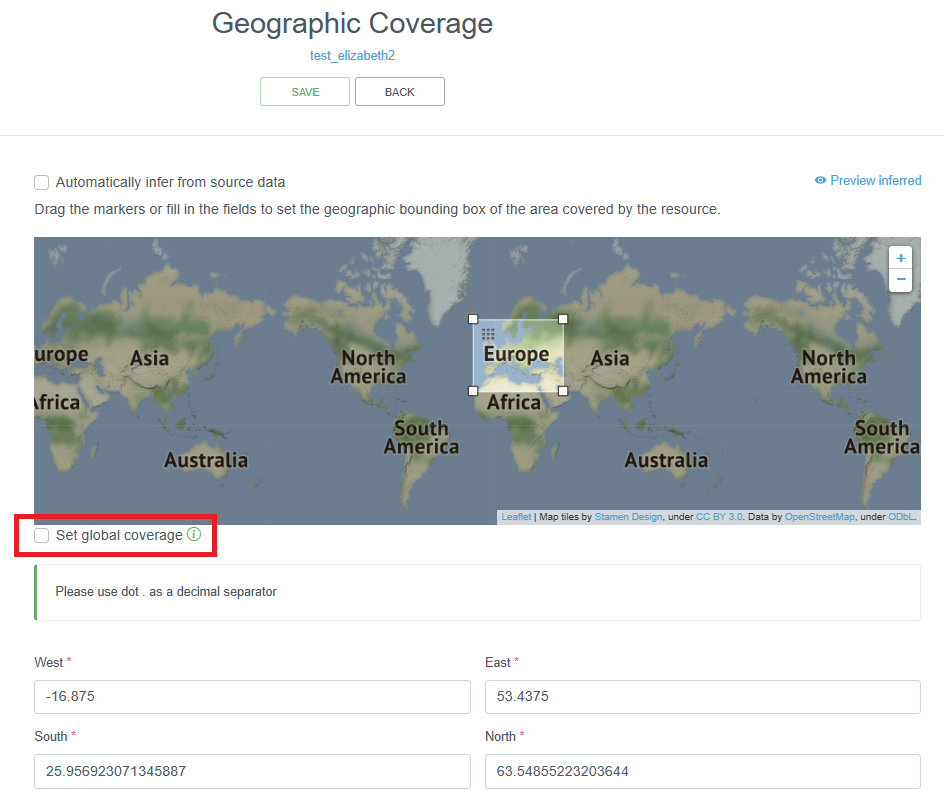
\includegraphics[width=0.6\textwidth,height=\textheight]{images/ipt-ss13-meta-geo.png}

}

\caption{Screenshot of the Geographical Coverage section of the
metadata, emphasizing how to change the bounds of the coverage box in
the map.}

\end{figure}

\hypertarget{taxonomic-coverage}{%
\subparagraph{Taxonomic Coverage}\label{taxonomic-coverage}}

This section can capture two things:

\begin{enumerate}
\def\labelenumi{\arabic{enumi}.}
\tightlist
\item
  A description of the range of taxa that are addressed in the data set.
  OBIS recommends to only add the higher classification (Kingdom, Class
  or Order) of the involved groups (e.g.~Bivalvia, Cetacea, Aves,
  Ophiuroidea\ldots). You can easily draw a list of higher taxonomic
  ranks from the WoRMS taxon match service (or ask the data provider).
  The taxonomic coverage is not a mandatory field, but the information
  stored here can be very useful as background information. The
  description can also contain common names, such as e.g.~benthic
  foraminifera or mussels.
\item
  An overview of all the involved taxa (not recommended, as all the taxa
  are already listed in the dataset).
\end{enumerate}

\begin{quote}
\emph{Note:} OBIS also recommends to add information on the (higher)
taxonomic groups in the (descriptive) dataset title and abstract.
\end{quote}

\begin{figure}

{\centering 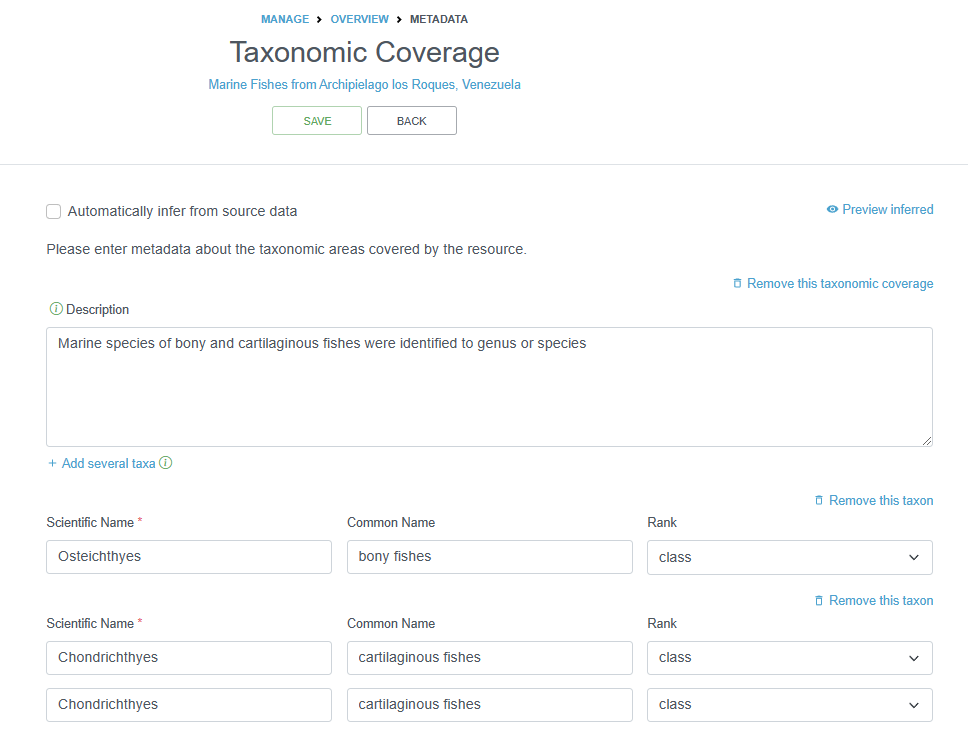
\includegraphics[width=0.7\textwidth,height=\textheight]{images/ipt-ss14-meta-taxa.png}

}

\caption{Example of the Taxonomic Coverage section of the metadata}

\end{figure}

\hypertarget{temporal-coverage}{%
\subparagraph{Temporal Coverage}\label{temporal-coverage}}

The temporal coverage will be a date range, which can easily be
documented. If it is a single date, the start and end date will be the
same. The information added here can be used as a quality check for the
actual dates in the datasets.

You can also document the Formation Period or the Living Time Period in
this section for specimens that may not have been alive during the
collection period, or to indicate the time during which the collection
occurred.

\begin{figure}

{\centering 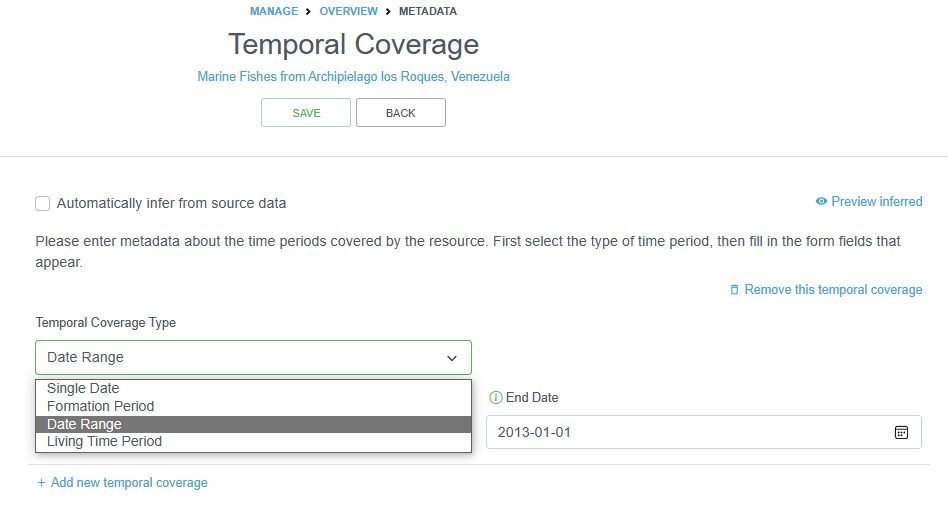
\includegraphics[width=0.7\textwidth,height=\textheight]{images/ipt-ss15-meta-time.png}

}

\caption{Example of the Temporal Coverage section of the metadata}

\end{figure}

\hypertarget{keywords}{%
\paragraph{Keywords}\label{keywords}}

Relevant keywords facilitate the discovery of a dataset. An indication
of the represented functional groups can help in a general search
(e.g.~plankton, benthos, zooplankton, phytoplankton, macrobenthos,
meiobenthos \ldots). Assigned keywords can be related to taxonomy,
habitat, geography or relevant keywords extracted from thesauri such as
the \href{https://vocabularyserver.com/asfa/}{ASFA thesaurus}, the
\href{http://www.cabi.org/cabthesaurus/}{CAB thesaurus} or
\href{https://www.earthdata.nasa.gov/learn/find-data/idn/gcmd-keywords}{GCMD
keywords}.

As taxonomy and geography are already covered in previous sections,
there is no need to repeat related keywords here. Please consult your
data provider which (relevant) keywords can be assigned.

\begin{figure}

{\centering 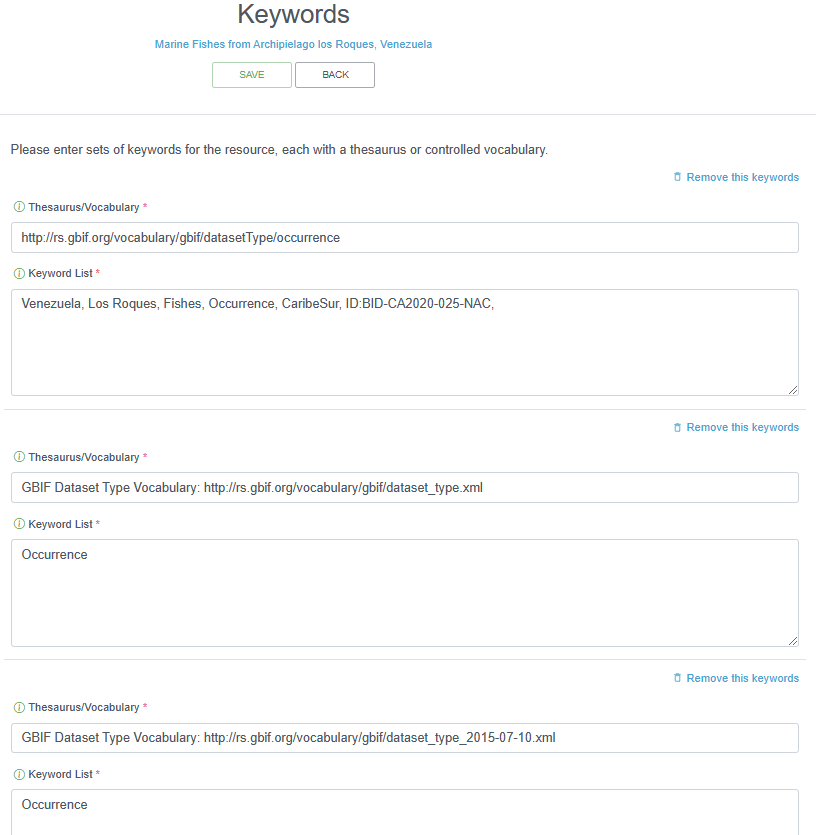
\includegraphics[width=0.7\textwidth,height=\textheight]{images/ipt-ss16-meta-keyword.png}

}

\caption{Example of the Keywords section of the metadata, showing input
for a marine fishes dataset}

\end{figure}

\hypertarget{project}{%
\paragraph{Project}\label{project}}

If the dataset in this resource is produced under a certain project, the
metadata on this project can be documented here. Part of the information
entered here, can partly overlap with information given in other
sections of the metadata (e.g.~study area description can have lot of
parallel with the geographic coverage section). Personnel involved in
the project can be documented or repeated here as well. This is not a
problem.

\hypertarget{sampling-methods}{%
\paragraph{Sampling Methods}\label{sampling-methods}}

The EML can contain descriptions of the sampling and data processing
methods. Study extent can be documented here as well to report a more
specific geographic area as well as the sampling frequency. Descriptions
of sampling procedures, quality control, and steps (sample or data
processing) can be given in the same way as the methods section of a
scientific paper.

Note that OBIS best practice is to add sampling facts to the extended
MeasurementorFact extension, linked to the sampling events in the Event
core via eventID.

\hypertarget{citations}{%
\paragraph{Citations}\label{citations}}

The dataset citation allows users to properly cite your dataset in
further publications or other uses of the data. When users download
datasets from the OBIS download function, a list of the dataset
citations packaged with the data in a zipped file is provided.

A dataset citation is different from the data source citation (in case
the data is digitized from a publication), and these references can be
added to the additional metadata (see bibliography below). A dataset
citation can have the same format of a journal article citation, and
should include the authors (contact, creator, principle investigator,
data managers, custodians, collectors\ldots), the title of the dataset,
the name of the data publisher (or custodian institute), and the access
point URL to the resource.

GBIF's IPT has an auto-generation - Turn On/Off - tool to let the IPT
auto-generate the resource citation for you. The citation includes a
version number, which is especially important for datasets that are
continuously updated. The dataset citation can also include a Citation
Identifier - a DOI, URI, or other persistent identifier that resolves to
an online dataset web page.

The OBIS node data managers should try to implement a certain degree of
format standardization for the dataset citations. The IPT provides an
option to auto-generate a citation based on the EML and is formatted as
follows: \{dataset.authors\} (\{dataset.pubDate\}) \{dataset.title\}.
{[}Version \{dataset.version\}{]}. \{organization.title\}.
\{dataset.type\} Dataset \{dataset.doi\}, \{dataset.url\}

\hypertarget{bibliography}{%
\paragraph{Bibliography}\label{bibliography}}

The EML can include the citation of the publications that are related to
the described dataset. They can describe the dataset, be based on the
dataset or be used in this dataset. Publications can be scientific
papers, reports, PhD or master theses. If available, the citation should
include the DOI at the end.

This overview will contribute to a better understanding of the data as
these publications can hold important additional information on the data
and how they were acquired.

\hypertarget{collection-data}{%
\paragraph{Collection Data}\label{collection-data}}

This IPT section should only be filled out if there are specimens held
in a museum. If relevant, it is strongly recommended that this
information is supplied by the data provider or left blank. The
collection name, specimen preservation method, and curatorial units
should be provided, as applicable.

\begin{figure}

{\centering 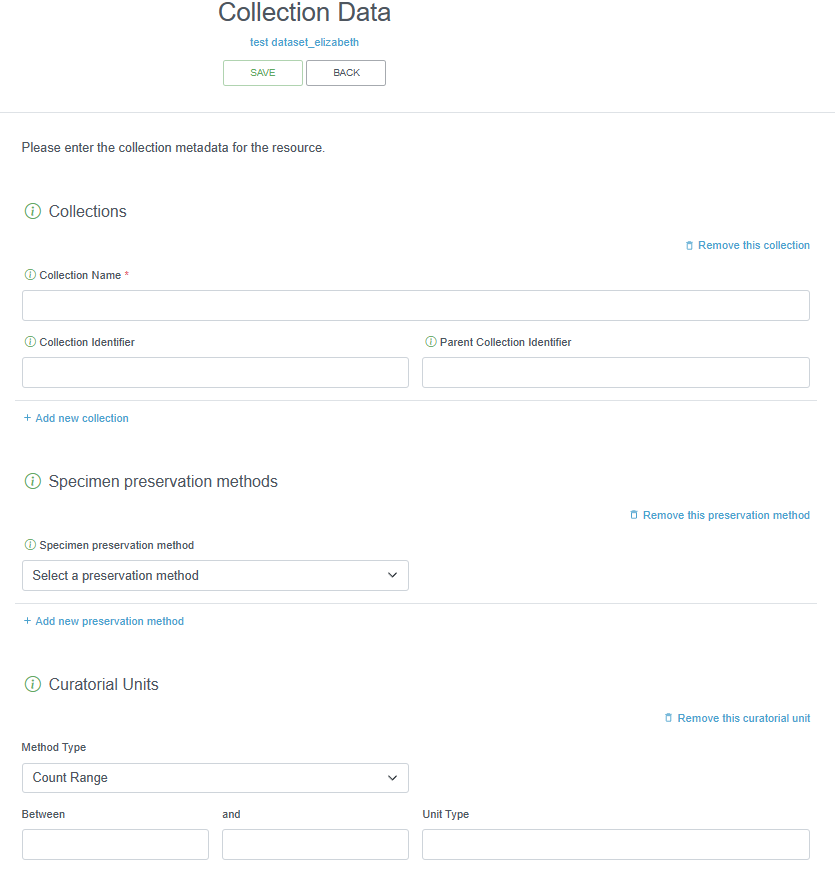
\includegraphics[width=0.7\textwidth,height=\textheight]{images/ipt-ss17-meta-collection.png}

}

\caption{Screenshot of the Collection Data page showing what information
can be provided for museum specimens}

\end{figure}

\hypertarget{external-links}{%
\paragraph{External Links}\label{external-links}}

This section can include URLs to the resource homepage, to download or
find additional information. You can also provide links to your resource
if it is hosted elsewhere in different formats.

Links to the online dataset on the OBIS website can be added once the
data is available there. For these OBIS links, the required fields
should be completed as follows:

\begin{itemize}
\tightlist
\item
  Name: online dataset
\item
  Character set: UTF-8
\item
  Data format: html
\end{itemize}

If other links are added, then the data format for web-based data is
`html'. If the link refers to a file, the data format of the file will
need to be added (e.g.~.xlsx, .pdf \ldots). The character set for all
Darwin Core files is UTF-8, whereas for other web pages this can vary,
so you may need to confirm.

\hypertarget{additional-metadata}{%
\paragraph{Additional Metadata}\label{additional-metadata}}

Any remaining information that could not be catalogued under any of the
other metadata, can be mentioned here. This may include logos, purpose
of the dataset, a description of how the dataset will be maintained,
etc.

\hypertarget{obis-nodes}{%
\section{OBIS nodes}\label{obis-nodes}}

\emph{Note the OBIS node TOR and system architecture is currently under
review and will be updated after the 2023 Steering Group meeting. The
information below may change.}

OBIS Nodes are either national projects, programmes, institutes, or
organizations, National Ocean Data Centers or regional or international
projects, programmes and institutions or organizations that carry out
data management functions.

OBIS nodes are responsible for \textbf{representing all aspects of OBIS
within a particular region or taxonomic domain}. Additional
responsibilities include:

\begin{itemize}
\tightlist
\item
  Establishing relationships with key data providers within their
  geographical (or taxonomic) area of responsibility
\item
  Bringing data and corresponding metadata into the global database to
  be shared with the OBIS community
\item
  Responsibility for \textbf{all aspects of the data}
\item
  Gaining permission to providing access to the data
\item
  Ensuring a certain level of data quality
\item
  Transfer of these datasets to the global OBIS database
\item
  Provide support for the full implementation of OBIS worldwide by
  serving on the IODE Steering Group for OBIS and any relevant Task
  Teams or ad hoc project teams
\item
  Each node may also maintain a data presence on the Internet
  representing their specific area of responsibility
\end{itemize}

\hypertarget{terms-of-reference-of-obis-nodes}{%
\subsection{Terms of Reference of OBIS
nodes}\label{terms-of-reference-of-obis-nodes}}

\textbf{Data Responsibilities}

\begin{itemize}
\tightlist
\item
  Receiving or harvesting marine biodiversity data (and metadata) from
  national, regional, and international programs, and the scientific
  community at large, and from Tier III nodes by Tier II nodes, and from
  Tier II nodes by Tier I nodes
\item
  Perform data validation (using standards, tools, and best practices),
  as described in the OBIS manual (Tier II)
\item
  Reporting the results of quality control directly to data
  collectors/originator (or Tier III node) as part of the quality
  assurance activity
\item
  Making data (and metadata) available to OBIS using agreed upon
  standards and formats which are described in the OBIS Manual (Tier
  II), making data available to Tier II nodes (Tier III)
\item
  Control data access, terms of use and sharing policies
\item
  Comply with the IOC/OBIS data policy for using and sharing OBIS data
\item
  Contribute to the development of standards and best practices in OBIS
  (recommended)
\item
  Contribute to the development of open-source tools in OBIS
  (recommended)
\item
  Ensuring the long-term preservation of the data, metadata and
  associated information required for correct interpretation of the data
  (including version-control) (recommended)
\item
  Build customized data portals (optional)
\end{itemize}

\textbf{Administration Responsibilities}

\begin{itemize}
\tightlist
\item
  Become a member of the IODE steering group for OBIS, attend the
  SG-OBIS annual meeting and report on node activities
\item
  Provide indicators on up-time, responsiveness, and data processed by
  nodes and present a report to SG-OBIS
\item
  Customer support (data queries, analyses, feedback)
\item
  Outreach and Capacity Building (i.e., providing expertise, training
  and support in data management, technologies, standards and best
  practices)
\item
  Engage in stakeholder groups (recommended)
\end{itemize}

\hypertarget{how-to-become-an-obis-node}{%
\subsection{How to become an OBIS
node}\label{how-to-become-an-obis-node}}

OBIS nodes now operate under the IODE network as either National
Oceanographic Data Centres (NODCs) or Associate Data Unites (ADUs).
Prospective nodes are required to apply to the IODE for membership.

The procedure to become an OBIS node is as follows:

\begin{itemize}
\tightlist
\item
  If you are an existing NODC (within the IODE network) and the OBIS
  node activities fall under the activities of the NODC:

  \begin{itemize}
  \tightlist
  \item
    Send a letter expressing your interest to become an OBIS node
    (including contact information of the OBIS node manager, and
    geographical/thematic scope of your OBIS node)
  \end{itemize}
\item
  If you are not an existing NODC:

  \begin{itemize}
  \tightlist
  \item
    Email your
    \href{http://iode.org/index.php?option=com_oe\&task=viewDocumentRecord\&docID=11793}{application
    form} to become an IODE Associate Data Unit (ADU), with a specific
    role as OBIS node. Applications for ADU membership in OBIS shall be
    reviewed by the IODE Officers in consultation with the IODE Steering
    Group for OBIS.
  \end{itemize}
\end{itemize}

\hypertarget{obis-node-health-status-check-and-transition-strategy}{%
\subsection{OBIS Node Health Status Check and Transition
Strategy}\label{obis-node-health-status-check-and-transition-strategy}}

OBIS nodes should operate under IODE as either IODE/ADU or IODE/NODC. As
such OBIS nodes are a member of the IODE network.

The IODE Steering Group (SG) for OBIS evaluates the health status of
OBIS nodes at each annual SG meeting, and considers an OBIS node as
\textbf{inactive} when it meets any of the following conditions:

\begin{enumerate}
\def\labelenumi{\arabic{enumi}.}
\tightlist
\item
  The OBIS node manager recurrently fails to answer the communications
  from the project manager or the SG co-chairs in the last 12 months
\item
  The OBIS node manager or a representative fails to attend (personally
  or virtually) the last 2 SG meetings without any written reason
\item
  The OBIS node does not have an IPT
\item
  The OBIS node has an IPT, but it has not been running for the last 12
  months
\item
  The datasets in the OBIS node's IPT have been removed and not restored
  in the last 12 months (without any explanation)
\item
  The OBIS node has not provided new data for the last 2 years
\end{enumerate}

The OBIS Secretariat prepares a health status check report of each OBIS
node based on the six items above and informs the OBIS node manager on
their status 3 months before the SG meeting. At the SG meeting, the
SG-OBIS co-chair will present the results of the OBIS nodes health
status check report including a listing of the inactive OBIS nodes. The
SG-OBIS members representing active OBIS Nodes will make one of the
following decisions:

\begin{enumerate}
\def\labelenumi{\arabic{enumi}.}
\tightlist
\item
  Request the inactive OBIS node to submit a plan with actions,
  deliverables and times to improve their performance, within 3 months,
  to the OBIS Secretariat. This plan is reviewed and accepted by the
  OBIS-Executive Committee Or
\item
  Provide a recommendation to the IOC Committee on IODE to remove the
  OBIS node from the IODE network.
\end{enumerate}

In either case, the OBIS Secretariat will inform the OBIS node manager
of the SG-OBIS decision, with a copy to the IODE officers and the IODE
national coordinator for data management of the country concerned.

The IODE Committee is requested to consider the recommendation from the
OBIS Steering Group and it may either accept the recommendation or
request the inactive OBIS node to submit an action plan (option 1).

When the inactive OBIS node is removed from the IODE network, the
SG-OBIS will ask whether another OBIS node is interested in taking over
the responsibilities of the removed OBIS node, until a new OBIS node in
the country/region is established.

\part{Data Formatting}

\hypertarget{dataset-structure}{%
\chapter{Dataset structure}\label{dataset-structure}}

Formatting data can be challenging. This section of the manual deals
with how to format data for OBIS, beginning with an overview of dataset
structure.

Deciding on your dataset structure is one of the first steps towards
getting your data ready for publishing. At this step, there are
different non arbitrary you need to do with your data, but it is
important to determine which structure best suits your dataset before
proceeding. Then, once you have decided on the dataset structure, you
can continue formatting your data.

We have created the following flow chart for an overview on how to
determine what structure best suits your data.

What kind of data do~ you have, or will collect?

What kind of data do\ldots{}

occurrence

occurrence

genetic

genetic

biomass

biomass

tracking

tracking

habitat

habitat

Do you have event level information (e.g.~sample, station, cruise,
study, etc.)?

Do you have event level infor\ldots{}

abundance, percent cover

abundance, perce\ldots{}

Yes

Yes

No

No

Have (or will) you collect any data associated with samples or sampling?
(e.g.~temperature, length, etc.)

Have (or will) you collec\ldots{}

Event core

Event core

Occurrence Core

Occurrence Core

Yes

Yes

No

No

Event core

Event core

Event core only

Event core\ldots{}

Occurrence Core

Occurrence Core

Have (or will) you collect any data associated with samples or sampling?
(e.g.~temperature, length, etc.)

Have (or will) you collec\ldots{}

Yes

Yes

No

No

Occurrence core

Occurrence\ldots{}

Occurrence core

Occurrence\ldots{}

DNAderived dataextension

DNA\ldots{}

Start

Start

eMoFextension

eMoF\ldots{}

eMoFextension

eMoF\ldots{}

Have (or will) you collect any data associated with samples or sampling?
(e.g.~temperature, length, etc.)

Have (or will) you collec\ldots{}

Yes

Yes

No

No

Occurrencecore

Occurrence\ldots{}

Occurrencecore only

Occurrence\ldots{}

eMoFextension

eMoF\ldots{}

DNAderived dataextension

DNA\ldots{}

DNAderived dataextension

DNA\ldots{}

Text is not SVG - cannot display

For more guidance, see the sections below.

\hypertarget{when-to-use-event-core}{%
\section{When to use Event Core}\label{when-to-use-event-core}}

Event Core describes \textbf{when} and \textbf{where} a specific
sampling event happened and contains information such as location and
date. Event Core is often used to organize your data tables when there
are more than one sampling occasion and/or location, and different
occurrences linked to each sampling. This organization follows the
rationale of most ecological studies and typical marine sampling design.
It covers:

\begin{itemize}
\tightlist
\item
  When specific details are known about \textbf{how} a biological sample
  was taken and processed. These details can then be defined in the eMoF
  Extension with the
  \href{https://www.bodc.ac.uk/resources/vocabularies/vocabulary_search/Q01/}{Q01
  vocabulary}
\item
  When the dataset contains abiotic measurements, or other biological
  measurements which are \textbf{related to an entire sample} (not a
  single specimen). For example a biomass measurement for an entire
  sample, not each species within the sample
\end{itemize}

Event Core can be used in combination with the Occurrence and eMoF
extensions. The identifier that links Event Core to the extension is the
\texttt{eventID}. \href{identifiers.html}{\texttt{parentID}} can also be
used to give information on hierarchical sampling. \texttt{occurrenceID}
can also be used in datasets with Event Core in order to link
information between the Occurrence extension and the eMoF extension.

\hypertarget{when-to-use-occurrence-core}{%
\section{When to use Occurrence
Core}\label{when-to-use-occurrence-core}}

Occurrence Core datasets describe \textbf{observations} and
\textbf{specimen records} and cover instances when:

\begin{itemize}
\tightlist
\item
  \textbf{No information} on how the data was sampled or how samples
  were processed is available
\item
  No abiotic measurements are taken or provided
\item
  You have \protect\hyperlink{edna-dna-derived-data}{eDNA and
  DNA-derived data}
\item
  Biological measurements are made on \textbf{individual specimens}
  (each specimen is a single occurrence record)
\end{itemize}

Occurrence Core is also often the preferred structure for museum
collections, citations of occurrences from literature, and sampling
activities.

Datasets formatted in Occurrence Core can use the eMoF Extension for
when you have biotic measurements or facts about your specimen. The DNA
derived data extension can also be used to link to DNA sequences. The
identifier that links Occurrence Core to the extension(s) is the
\texttt{occurrenceID}.

\hypertarget{extensions-in-obis}{%
\section{Extensions in OBIS}\label{extensions-in-obis}}

Currently OBIS accepts the following extensions:

\begin{itemize}
\tightlist
\item
  Occurrence
\item
  Event
\item
  MeasurementOrFact
\item
  extendedMeasurementOrFact
\item
  DNADerivedData
\end{itemize}

\hypertarget{how-are-extensions-linked-to-core-tables-in-obis}{%
\subsection{How are extensions linked to core tables in
OBIS?}\label{how-are-extensions-linked-to-core-tables-in-obis}}

As established in the \href{relational_db.html}{relational database
section}, OBIS relies on datasets being formatted according to a
relational database structure. The
\protect\hyperlink{obis-holds-more-than-just-species-occurrences-the-env-data-approach}{ENV-DATA
approach} that OBIS implements means your dataset will have a Core table
and (optionally) Extension tables. As a review, a core file contains
information relevant and applicable to each record in the extension(s).
An extension file then contains records that link back to a record in
the core file with more specific information (e.g., methods,
measurements, facts, DNA sequences, etc.).

The extension file(s) accepted by OBIS (eMoF, Occurrence, DNA) are
linked to your core tables by the use of identifying ID codes. These
codes could be either \texttt{eventID} or \texttt{occurrenceID}. For
details on how to construct these IDs, click
\href{identifiers.html}{here}.

\hypertarget{differences-between-identifiers}{%
\subsection{Differences between
identifiers}\label{differences-between-identifiers}}

If your core file is based on occurrences (e.g., a record of one or more
taxa specimens), then any extensions are linked with
\texttt{occurrenceID}. If your core file is based on events (e.g., a
sampling event, cruise, observation, etc.), then the linking identifier
is \texttt{eventID}. In the Core tables, identifiers are always unique,
which means, they do not repeat and each line has a different
identifier. On the other hand, multiple records in an extension file can
have the same identifier which will link them to the same event or
occurrence record (depending on which is the Core). The different
linking identifiers are shown in the figure below.

\begin{figure}

{\centering 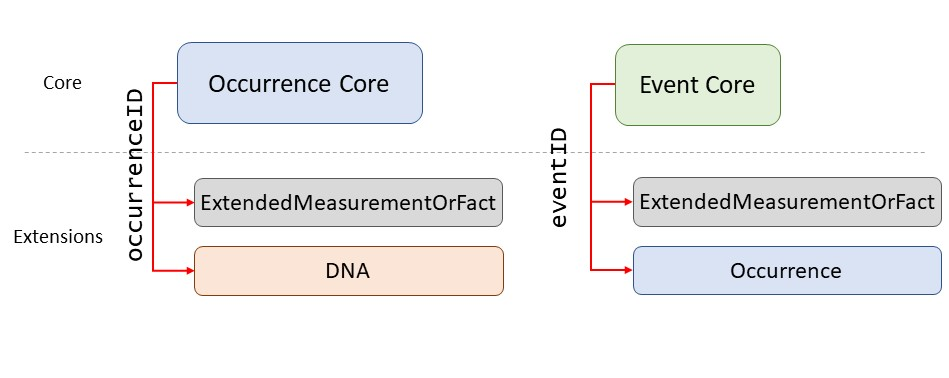
\includegraphics[width=0.5\textwidth,height=\textheight]{images/coretable-identifiers.jpg}

}

\caption{Diagram of how the different core tables are linked to their
extensions by different identifiers.}

\end{figure}

Let us consider a fictional plankton trawl sampling event to demonstrate
how identifiers link Core and Extension tables in OBIS. This trawl used
two types of nets, occurred in March 2013, and has an eventID
\texttt{plankton-northsea-2013-03}. Suppose we have information about
the types of trawl used and the species abundance from this trawling
event. The information (e.g., date) of the sampling event itself would
be found in the Event Core, whereas the abundance data and sampling
methods would be in the eMoF table. How do we ensure the abundance and
sampling method data is properly linked to the correct event? By using
the same eventID for each record in the eMoF table,
\texttt{plankton-northsea-2013-03}, the information is properly linked
between the Event Core and the eMoF extension.

\hypertarget{data-formatting-tools}{%
\section{Data formatting tools}\label{data-formatting-tools}}

The GBIF Norwegian Node created the
\href{https://gbif-norway.github.io/dwc-excel-template-generator-js/}{DwC
Excel Template Generator}. This tool will generate four different types
of blank Excel spreadsheets: Occurrence Core, MeasurementOrFact,
Metadata, and a README. This tool works best if you already know which
Darwin Core fields you need, although a default template can be
generated.

Another tool from Norway is the
\href{https://zenodo.org/record/6453921\#.Y9KsQkHMKmU}{Excel to Darwin
Core Standard (DwC) Tool}. This is a macro Excel spreadsheet that helps
create templates for Event (aka Sampling-Event) and Occurrence core
tables, as well as MeasurementsOrFacts, Extended MeasurementsOrFacts,
and Simple Multimedia extensions. GBIF provides an
\href{https://ipt.gbif.org/manual/en/ipt/latest/occurrence-data\#templates}{Occurrence
core template} and an
\href{https://ipt.gbif.org/manual/en/ipt/latest/sampling-event-data\#templates}{Event
core template}. If you use these templates from GBIF, be aware that
\protect\hyperlink{differences-between-obis-and-gbif-publication-processes}{GBIF's
required terms are different from OBIS}.

There are also some tools that can help you unpivot (or flatten) data
tables. These can be used to flatten many columns into one, particularly
useful for the \href{format_emof.html}{eMoF} table.

\begin{itemize}
\tightlist
\item
  \href{https://gbif-norway.github.io/crosstab2list/}{GBIF Norway's
  crosstab to list converter}. Note that this tool is not completely
  automated
\item
  \href{https://www.excel-university.com/unpivot-excel-data/}{Excel's
  built-in unpivot function}
\end{itemize}

\hypertarget{formatting-data-tables}{%
\chapter{Formatting data tables}\label{formatting-data-tables}}

\hypertarget{darwin-core-term-checklist-for-obis}{%
\section{Darwin Core Term Checklist for
OBIS}\label{darwin-core-term-checklist-for-obis}}

There are many Darwin Core terms listed in the
\href{https://dwc.tdwg.org/terms/}{TDWG quick reference guide}. However,
not all these terms are necessary for publishing data to OBIS.

For your convenience, we have created a checklist of all the Darwin Core
terms relevant for OBIS data providers. You can reference this list to
quickly see which terms are required by OBIS, which file (Event,
Occurrence, eMoF, DNA) they can be found in, and which Darwin Core class
it relates to. These terms correlate with the
\protect\hyperlink{map-your-data-to-darwin-core}{IPT vocabulary mapping}
you will do when it comes time to publish your dataset. You may notice
some terms are accepted in multiple data tables (e.g., Event and
Occurrence) - this is because it depends on your dataset structure. If
you have an Event Core, you will include some terms that would not be
included if you had Occurrence Core. For guidance on specific class
terms (e.g., location, taxonomy, etc.), see the
\protect\hyperlink{darwin-core-guidelines}{Darwin Core} section of the
manual.

Note that when you publish your dataset on the IPT, if you use a term
not listed below it will be an unmapped field and will \textbf{not} be
published alongside your data. You may still wish to include such fields
in your dataset if you are publishing to other repositories, just know
that they will not be included in your OBIS dataset. You may include
this information either by putting it in the \texttt{dynamicProperties}
field in JSON format, or putting the information into the
\href{format_emof.html}{eMoF}. Alternatively, you may have fields that
you do not wish to be published and that do not correspond to one of
these terms (e.g.~personal notes). This is okay - if they are not mapped
to one of the terms, that column in your dataset will not be published.

\begin{longtable}[]{@{}
  >{\raggedright\arraybackslash}p{(\columnwidth - 12\tabcolsep) * \real{0.1343}}
  >{\raggedright\arraybackslash}p{(\columnwidth - 12\tabcolsep) * \real{0.1642}}
  >{\raggedright\arraybackslash}p{(\columnwidth - 12\tabcolsep) * \real{0.1343}}
  >{\raggedright\arraybackslash}p{(\columnwidth - 12\tabcolsep) * \real{0.1493}}
  >{\raggedright\arraybackslash}p{(\columnwidth - 12\tabcolsep) * \real{0.1194}}
  >{\raggedright\arraybackslash}p{(\columnwidth - 12\tabcolsep) * \real{0.1493}}
  >{\raggedright\arraybackslash}p{(\columnwidth - 12\tabcolsep) * \real{0.1493}}@{}}
\toprule\noalign{}
\begin{minipage}[b]{\linewidth}\raggedright
Term
\end{minipage} & \begin{minipage}[b]{\linewidth}\raggedright
OBIS Required
\end{minipage} & \begin{minipage}[b]{\linewidth}\raggedright
DarwinCore Class
\end{minipage} & \begin{minipage}[b]{\linewidth}\raggedright
Event
\end{minipage} & \begin{minipage}[b]{\linewidth}\raggedright
Occurrence
\end{minipage} & \begin{minipage}[b]{\linewidth}\raggedright
eMoF
\end{minipage} & \begin{minipage}[b]{\linewidth}\raggedright
DNA
\end{minipage} \\
\midrule\noalign{}
\endhead
\bottomrule\noalign{}
\endlastfoot
eventDate & required & event & x & x & & \\
eventID & required & event & x & x & x & \\
decimalLatitude & required & location & x & x & & \\
decimalLongitude & required & location & x & x & & \\
occurrenceID & required & occurrence & & x & x & x \\
occurrenceStatus & required & occurrence & & x & & \\
basisOfRecord & required & record & & x & & x \\
scientificName & required & taxon & & x & & \\
scientificNameID & strongly recommended & taxon & & x & & \\
DNA\_sequence & strongly recommended & dna & & & & x \\
env\_broad\_scale & strongly recommended & dna & & & & x \\
env\_local scale & recommended & dna & & & & x \\
env\_medium & strongly recommended & dna & & & & x \\
lib\_layout & recommended & dna & & & & x \\
nucl\_acid\_amp & recommended & dna & & & & x \\
nucl\_acid\_ext & recommended & dna & & & & x \\
otu\_class\_appr & recommended & dna & & & & x \\
otu\_db & recommended & dna & & & & x \\
otu\_seq\_comp\_appr & recommended & dna & & & & x \\
pcr\_primer\_forward & strongly recommended & dna & & & & x \\
pcr\_primer\_name\_forward & strongly recommended & dna & & & & x \\
pcr\_primer\_name\_reverse & strongly recommended & dna & & & & x \\
pcr\_primer\_reference & strongly recommended & dna & & & & x \\
pcr\_primer\_reverse & strongly recommended & dna & & & & x \\
samp\_name & recommended & dna & & & & x \\
samp\_vol\_we\_dna\_ext & recommended & dna & & & & x \\
seq\_meth & recommended & dna & & & & x \\
sop & recommended & dna & & & & x \\
target\_gene & strongly recommended & dna & & & & x \\
target\_subfragment & strongly recommended & dna & & & & x \\
day & recommended & event & x & x & & \\
endDayOfYear & recommended & event & x & x & & \\
eventRemarks & optional & event & x & x & & \\
eventTime & recommended & event & x & x & & \\
fieldNotes & optional & event & x & & & \\
fieldNumber & optional & event & x & & & \\
habitat & recommended & event & x & & x & \\
month & strongly recommended & event & x & x & & \\
parentEventID & required (if exists) & event & x & & & \\
sampleSizeUnit & strongly recommended & event & & x & x & \\
sampleSizeValue & strongly recommended & event & & x & x & \\
samplingEffort & strongly recommended & event & & x & x & \\
samplingProtocol & strongly recommended & event & & x & x & \\
startDayOfYear & recommended & event & x & & & \\
verbatimEventDate & recommended & event & x & & & \\
year & strongly recommended & event & x & x & & \\
bed & optional & geologicalContext & x & x & & \\
earliestAgeOrLowestStage & optional & geologicalContext & x & x & & \\
earliestEonOrLowestEonothem & optional & geologicalContext & x & x &
& \\
earliestEpochOrLowestSeries & optional & geologicalContext & x & x &
& \\
earliestEraOrLowestErathem & optional & geologicalContext & x & x & & \\
earliestPeriodOrLowestSystem & optional & geologicalContext & x & x &
& \\
formation & optional & geologicalContext & x & x & & \\
group & optional & geologicalContext & x & x & & \\
highestBiostratigraphicZone & optional & geologicalContext & x & x &
& \\
latestAgeOrHighestStage & optional & geologicalContext & x & x & & \\
latestEonOrHighestEonothem & optional & geologicalContext & x & x & & \\
latestEpochOrHighestSeries & optional & geologicalContext & x & x & & \\
latestEraOrHighestErathem & optional & geologicalContext & x & x & & \\
latestPeriodOrHighestSystem & optional & geologicalContext & x & x &
& \\
lithostratigraphicTerms & optional & geologicalContext & x & x & & \\
lowestBiostratigraphicZone & optional & geologicalContext & x & x & & \\
member & optional & geologicalContext & x & x & & \\
dateIdentified & optional & identification & & x & & \\
identificationID & optional & identification & & x & & \\
identificationQualifier & recommended & identification & & x & & \\
identificationReferences & optional (required for imaging data) &
identification & & x & & \\
identificationRemarks & recommended & identification & & x & & \\
identificationVerificationStatus & optional (required for imaging data)
& identification & & x & & \\
identifiedBy & optional (required for imaging data) & identification & &
x & & \\
identifiedByID & optional & identification & & x & & \\
typeStatus & optional & identification & & x & & \\
continent & strongly recommended & location & x & x & & \\
coordinatePrecision & strongly recommended & location & x & x & & \\
coordinateUncertaintyInMeters & strongly recommended & location & x & x
& & \\
country & recommended & location & x & x & & \\
countryCode & optional & location & x & x & & \\
county & optional & location & x & x & & \\
footprintSpatialFit & optional & location & x & x & & \\
footprintSRS & optional & location & x & x & & \\
footprintWKT & recommended & location & x & x & & \\
geodeticDatum & recommended & location & x & x & & \\
georeferencedBy & optional & location & x & x & & \\
georeferencedDate & optional & location & x & x & & \\
georeferenceProtocol & optional & location & x & x & & \\
georeferenceSources & optional & location & x & x & & \\
higherGeography & optional & location & x & x & & \\
higherGeographyID & optional & location & x & x & & \\
island & optional & location & x & x & & \\
islandGroup & optional & location & x & x & & \\
locality & recommended & location & x & x & & \\
locationAccordingTo & recommended & location & x & x & & \\
locationID & strongly recommended & location & x & x & & \\
locationRemarks & recommended & location & x & x & & \\
maximumDepthInMeters & strongly recommended & location & x & x & & \\
maximumDistanceAboveSurfaceInMeters & optional & location & x & x & & \\
maximumElevationInMeters & optional & location & x & x & & \\
minimumDepthInMeters & strongly recommended & location & x & x & & \\
minimumDistanceAboveSurfaceInMeters & optional & location & x & x & & \\
minimumElevationInMeters & optional & location & x & x & & \\
municipality & optional & location & x & x & & \\
pointRadiusSpatialFit & optional & location & x & x & & \\
stateProvince & optional & location & x & x & & \\
verbatimCoordinates & optional & location & x & x & & \\
verbatimCoordinateSystem & optional & location & x & x & & \\
verbatimDepth & optional & location & x & x & & \\
verbatimElevation & optional & location & x & x & & \\
verbatimLatitude & optional & location & x & x & & \\
verbatimLocality & optional & location & x & x & & \\
verbatimLongitude & optional & location & x & x & & \\
verbatimSRS & optional & location & x & x & & \\
waterBody & recommended & location & x & x & & \\
materialSampleID & recommended & materialSample & & x & & \\
measurementAccuracy & recommended & measurementOrFact & & & x & \\
measurementDeterminedBy & optional & measurementOrFact & & & x & \\
measurementDeterminedDate & optional & measurementOrFact & & & x & \\
measurementID & recommended & measurementOrFact & & & x & \\
measurementMethod & recommended & measurementOrFact & & & x & \\
measurementRemarks & recommended & measurementOrFact & & & x & \\
measurementType & strongly recommended & measurementOrFact & & & x & \\
measurementTypeID & strongly recommended & measurementOrFact & & & x
& \\
measurementUnit & strongly recommended & measurementOrFact & & & x & \\
measurementUnitID & strongly recommended & measurementOrFact & & & x
& \\
measurementValue & strongly recommended & measurementOrFact & & & x & \\
measurementValueID & strongly recommended & measurementOrFact & & & x
& \\
associatedMedia & recommended & occurrence & & x & & \\
associatedReferences & optional & occurrence & & x & & \\
associatedSequences & recommended & occurrence & & x & & \\
associatedTaxa & optional & occurrence & & x & & \\
behavior & recommended & occurrence & & x & x & \\
catalogNumber & recommended & occurrence & & x & & \\
disposition & optional & occurrence & & x & & \\
establishmentMeans & optional & occurrence & & x & & \\
georeferenceVerificationStatus & recommended & occurrence & & x & & \\
individualCount & strongly recommended & occurrence & & x & x & \\
lifeStage & recommended & occurrence & & x & x & \\
occurrenceRemarks & recommended & occurrence & & x & & \\
organismQuantity & strongly recommended & occurrence & & x & x & \\
organismQuantityType & strongly recommended & occurrence & & x & x & \\
otherCatalogNumbers & optional & occurrence & & x & & \\
preparations & optional & occurrence & & x & & \\
recordedBy & recommended & occurrence & & x & & \\
recordedByID & recommended & occurrence & & x & & \\
recordNumber & recommended & occurrence & & x & & \\
reproductiveCondition & recommended & occurrence & & x & & \\
sex & recommended & occurrence & & x & x & \\
associatedOccurrences & optional & organsim & & x & & \\
associatedOrganisms & optional & organsim & & x & & \\
organismID & recommended & organsim & & x & & \\
organismName & recommended & organsim & & x & & \\
organismRemarks & recommended & organsim & & x & & \\
organismScope & optional & organsim & & x & & \\
previousIdentifications & recommended & organsim & & x & & \\
accessRights & recommended & record & x & x & & \\
bibliographicCitation & recommended & record & x & x & & \\
collectionCode & optional & record & x & x & & \\
collectionID & optional & record & x & x & & \\
dataGeneralizations & optional & record & x & x & & \\
datasetID & recommended & record & x & x & & \\
datasetName & recommended & record & x & x & & \\
dynamicProperties & recommended & record & x & x & & \\
informationWithheld & optional & record & x & x & & \\
institutionCode & optional & record & x & x & & \\
institutionID & optional & record & x & x & & \\
language & recommended & record & x & x & & \\
license & recommended & record & x & x & & \\
modified & recommended & record & x & x & & \\
ownerInstitutionCode & optional & record & x & x & & \\
references & recommended & record & x & x & & \\
rightsHolder & recommended & record & x & x & & \\
type & strongly recommended & record & x & x & x & \\
acceptedNameUsage & recommended & taxon & & x & & \\
acceptedNameUsageID & recommended & taxon & & x & & \\
higherClassification & recommended & taxon & & x & & \\
infraspecificEpithet & recommended & taxon & & x & & \\
nameAccordingToID & recommended & taxon & & x & & \\
namePublishedInID & optional & taxon & & x & & \\
namePublishedInYear & optional & taxon & & x & & \\
nomenclaturalCode & optional & taxon & & x & & \\
nomenclaturalStatus & optional & taxon & & x & & \\
originalNameUsage & recommended & taxon & & x & & \\
originalNameUsageID & recommended & taxon & & x & & \\
parentNameUsage & recommended & taxon & & x & & \\
parentNameUsageID & recommended & taxon & & x & & \\
phylum & recommended & taxon & & x & & \\
scientificNameAuthorship & recommended & taxon & & x & & \\
specificEpithet & recommended & taxon & & x & & \\
subgenus & recommended & taxon & & x & & \\
taxonConceptID & optional & taxon & & x & & \\
taxonID & optional & taxon & & x & & \\
taxonomicStatus & optional & taxon & & x & & \\
taxonRank & strongly recommended & taxon & & x & & \\
taxonRemarks & recommended & taxon & & x & & \\
verbatimTaxonRank & recommended & taxon & & x & & \\
vernacularName & recommended & taxon & & x & & \\
type or eventType & strongly recommended & event & x & & & \\
class & recommended & taxon & & x & & \\
family & recommended & taxon & & x & & \\
genus & strongly recommended & taxon & & x & & \\
kingdom & strongly recommended & taxon & & x & & \\
order & strongly recommended & taxon & & x & & \\
\end{longtable}

\part{Ensuring Data Quality}

\hypertarget{data-quality-control}{%
\chapter{Data quality control}\label{data-quality-control}}

OBIS ignores records that do not meet a number of standards. For
example, all species names need to be matched against an authoritative
taxonomic register, such as the World Register of Marine Species. In
addition, quality is checked against the OBIS required fields as well as
against any impossible values. OBIS checks, rejects and reports the data
quality back to the OBIS nodes, but never change records. The OBIS tier
2 nodes are responsible for the data quality and communicate errors back
to the data providers. A number of QC tools are developed to help data
providers and OBIS nodes:

\begin{itemize}
\tightlist
\item
  \href{name_matching.html}{QC tool for species names}
\item
  \href{lifewatch_qc.html}{QC tool for geography and data format}
\end{itemize}

For specific concerns regarding quality control checks or issues, please
submit a GitHub ticket to the
\href{https://github.com/iobis/obis-qc/issues}{OBIS QC repository}.

\hypertarget{why-are-records-dropped}{%
\section{Why are records dropped?}\label{why-are-records-dropped}}

Records can be dropped and therefore not published with your dataset for
a number of reasons, including:

\begin{itemize}
\tightlist
\item
  The species is not marine
\item
  The `scientificName' or \texttt{scientificNameID} did not match with
  WoRMS
\item
  Issues with coordinates:

  \begin{itemize}
  \tightlist
  \item
    No coordinates given
  \item
    \texttt{decimalLatitude} or \texttt{decimalLongitude} out of range
  \end{itemize}
\item
  The coordinate is zero
\end{itemize}

For each dataset published, a quality report is generated where the
number of dropped records and other quality issues will be flagged. Such
reports can also be found when searching for data in OBIS. For example,
if we searched for `Crustacea' records, the following data quality
report is given:

\begin{figure}

{\centering 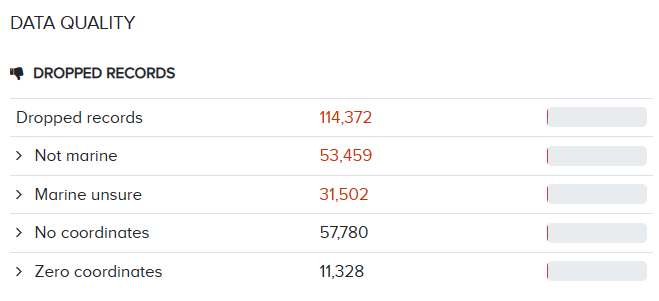
\includegraphics{images/crustacean-droppedrecords.png}

}

\caption{Number of Crustacean records dropped}

\end{figure}

We can see that \textgreater110,222 Crustacean records have been
dropped, mostly due to records missing coordinates or species being
flagged as non-marine. Because species are determined as being marine by
WoRMS, we acknowledge that sometimes species are marked as
\texttt{not\_marine} erroneously.For specific advice on this topic, see
the \protect\hyperlink{non-marine-species}{common QC issues page}.

To minimize the number of records dropped, be careful when formatting
your data so that you are meeting the requirements.

\hypertarget{how-to-conduct-quality-control}{%
\section{How to conduct Quality
Control}\label{how-to-conduct-quality-control}}

Once you have formatted your data for OBIS, or have received a formatted
dataset, it is important to run quality control checks before publishing
the dataset on the IPT. The following is a list of various tools you can
use to help you perform quality checks on your data:

\begin{itemize}
\tightlist
\item
  R package \href{https://github.com/iobis/obistools}{obistools}
\item
  EMODnet Biocheck

  \begin{itemize}
  \tightlist
  \item
    \href{https://rshiny.lifewatch.be/BioCheck/}{Web UI} built on
    obistools. This tool requires your dataset to be published on an IPT
    (e.g., a test IPT such as \url{https://ipt.gbif.org/} where your
    dataset will not be harvested by GBIF or OBIS). Note you are
    \href{ipt.html}{required to have a login} to access an IPT
  \item
    \href{https://github.com/EMODnet/EMODnetBiocheck}{R package}
  \end{itemize}
\item
  \href{https://www.lifewatch.be/data-services/}{Lifewatch data
  services}
\item
  The US Integrated Ocean Observing System
  \href{https://github.com/ioos/bio_data_guide/blob/main/datasets/TPWD_HARC_BagSeine/TPWD_HARC_BagSeine_OBISENV.md}{Standardizing
  Marine Bio Data Guide}
\item
  \href{https://www.marinespecies.org/aphia.php?p=match}{WoRMS taxon
  match tool}

  \begin{itemize}
  \tightlist
  \item
    \href{https://www.marinespecies.org/aphia.php?p=webservice}{Other
    WoRMS web services, incl.~taxon match}
  \end{itemize}
\item
  Excel Conditional Formatting tool

  \begin{itemize}
  \tightlist
  \item
    Excel \textgreater{} Home \textgreater{} Conditional Formating
    \textgreater{} Highlight cells Rules \textgreater{} Duplicate
    values\ldots{}
  \end{itemize}
\item
  \href{https://www.gbif.org/tools/data-validator}{GBIF data validator}
\item
  \href{https://github.com/cioos-siooc/pyobistools}{Python library for
  OBIS QC} developed by Canadian Integrated Ocean Observing System
\item
  R package and function Hmisc:: describe

  \begin{itemize}
  \tightlist
  \item
    Can give important summary statistics and identify numbers that
    don't match
  \end{itemize}
\end{itemize}

\hypertarget{conducting-qc-with-obistools}{%
\subsection{Conducting QC with
obistools}\label{conducting-qc-with-obistools}}

To use \texttt{obistools} to conduct quality control, you can follow
this general order:

\begin{enumerate}
\def\labelenumi{\arabic{enumi}.}
\tightlist
\item
  Check that the taxa match with WoRMS

  \begin{itemize}
  \tightlist
  \item
    \href{https://github.com/iobis/obistools\#taxon-matching}{\texttt{obistools::match\_taxa}}
  \end{itemize}
\item
  Check that all required fields are present in the occurrence table

  \begin{itemize}
  \tightlist
  \item
    \href{https://github.com/iobis/obistools\#check-required-fields}{\texttt{obistools::check\_fields}}
  \end{itemize}
\item
  Check coordinates

  \begin{itemize}
  \tightlist
  \item
    Plot them on a map to identify any points that appear outside the
    scope of the dataset
    \href{https://github.com/iobis/obistools\#plot-points-on-a-map}{\texttt{obistools::plot\_map}}
  \item
    Identify points with obistools::identify\_map
  \item
    Check that points are not on land
    \href{https://github.com/iobis/obistools\#check-points-on-land}{\texttt{obistools::check\_onland}}
  \item
    Ensure depth ranges are valid
    \href{https://github.com/iobis/obistools\#check-depth}{\texttt{obistools::check\_depth}}
  \end{itemize}
\item
  Check for
  \href{https://github.com/iobis/obistools\#check-outliers}{statistical
  outliers} which may have had data entry errors

  \begin{itemize}
  \tightlist
  \item
    obistools::check\_outliers\_species and
    obistools::check\_outliers\_dataset
  \end{itemize}
\item
  Check that the eventID and parentEventID are structured correctly
  \href{https://github.com/iobis/obistools\#check-outliers}{\texttt{obistools::check\_eventids}}

  \begin{itemize}
  \tightlist
  \item
    Ensure all eventIDs in extensions have matching eventIDs in the core
    table
    \href{https://github.com/iobis/obistools\#check-eventid-in-an-extension}{\texttt{obistools::check\_extension\_eventids}}
  \end{itemize}
\item
  Check that eventDate is formatted properly
  \href{https://github.com/iobis/obistools\#check-eventdate}{\texttt{obistools::check\_eventdate}}
\end{enumerate}

\hypertarget{qc-with-r-package-hmisc}{%
\subsection{QC with R package Hmisc}\label{qc-with-r-package-hmisc}}

The R package
\href{https://cran.r-project.org/web/packages/Hmisc/index.html}{Hmisc}
has the function
\href{https://rdrr.io/cran/Hmisc/man/describe.html}{\texttt{describe}}
which can help you identify any discrepancies in your dataset.

It will summarize each of your variables for a given data field. This
can help you quickly identify any missing data and ensure the number of
unique IDs is correct. For example, in an Occurrence table with 1000
records, there should be 1000 unique occurrenceIDs.

\begin{Shaded}
\begin{Highlighting}[]
\FunctionTok{library}\NormalTok{(Hmisc)}
\FunctionTok{library}\NormalTok{(Hmisc)}
\NormalTok{data}\OtherTok{\textless{}{-}}\FunctionTok{read.csv}\NormalTok{(}\StringTok{"example\_data\_occur.csv"}\NormalTok{)}
\FunctionTok{describe}\NormalTok{(data)}
 
 \DecValTok{12}\NormalTok{  Variables      }\DecValTok{407}\NormalTok{  Observations}
\SpecialCharTok{{-}{-}{-}{-}{-}{-}{-}{-}{-}{-}{-}{-}{-}{-}{-}{-}{-}{-}{-}{-}{-}{-}{-}{-}{-}{-}{-}{-}{-}{-}{-}{-}{-}{-}{-}{-}{-}{-}{-}{-}{-}{-}{-}{-}{-}{-}{-}{-}{-}{-}{-}{-}{-}{-}{-}{-}{-}{-}{-}{-}{-}{-}{-}{-}{-}{-}{-}{-}{-}{-}{-}{-}{-}{-}{-}{-}{-}{-}{-}{-}{-}{-}{-}{-}{-}{-}{-}{-}{-}{-}{-}{-}{-}{-}{-}{-}{-}{-}{-}{-}{-}{-}{-}{-}{-}{-}{-}{-}{-}{-}{-}{-}{-}{-}}
\NormalTok{CollectionCode }
\NormalTok{       n  missing distinct    value }
     \DecValTok{407}        \DecValTok{0}        \DecValTok{1}\NormalTok{  BIOFUN1 }
                  
\NormalTok{Value      BIOFUN1}
\NormalTok{Frequency      }\DecValTok{407}
\NormalTok{Proportion       }\DecValTok{1}
\SpecialCharTok{{-}{-}{-}{-}{-}{-}{-}{-}{-}{-}{-}{-}{-}{-}{-}{-}{-}{-}{-}{-}{-}{-}{-}{-}{-}{-}{-}{-}{-}{-}{-}{-}{-}{-}{-}{-}{-}{-}{-}{-}{-}{-}{-}{-}{-}{-}{-}{-}{-}{-}{-}{-}{-}{-}{-}{-}{-}{-}{-}{-}{-}{-}{-}{-}{-}{-}{-}{-}{-}{-}{-}{-}{-}{-}{-}{-}{-}{-}{-}{-}{-}{-}{-}{-}{-}{-}{-}{-}{-}{-}{-}{-}{-}{-}{-}{-}{-}{-}{-}{-}{-}{-}{-}{-}{-}{-}{-}{-}{-}{-}{-}{-}{-}{-}}
\NormalTok{eventID }
\NormalTok{       n  missing distinct }
     \DecValTok{407}        \DecValTok{0}       \DecValTok{27} 

\NormalTok{lowest }\SpecialCharTok{:}\NormalTok{ BIOFUN1\_BF1A01 BIOFUN1\_BF1A02 BIOFUN1\_BF1A03 BIOFUN1\_BF1A04 BIOFUN1\_BF1A05}
\NormalTok{highest}\SpecialCharTok{:}\NormalTok{ BIOFUN1\_BF1M3  BIOFUN1\_BF1M4  BIOFUN1\_BF1M6  BIOFUN1\_BF1M8  BIOFUN1\_BF1M9 }
\SpecialCharTok{{-}{-}{-}{-}{-}{-}{-}{-}{-}{-}{-}{-}{-}{-}{-}{-}{-}{-}{-}{-}{-}{-}{-}{-}{-}{-}{-}{-}{-}{-}{-}{-}{-}{-}{-}{-}{-}{-}{-}{-}{-}{-}{-}{-}{-}{-}{-}{-}{-}{-}{-}{-}{-}{-}{-}{-}{-}{-}{-}{-}{-}{-}{-}{-}{-}{-}{-}{-}{-}{-}{-}{-}{-}{-}{-}{-}{-}{-}{-}{-}{-}{-}{-}{-}{-}{-}{-}{-}{-}{-}{-}{-}{-}{-}{-}{-}{-}{-}{-}{-}{-}{-}{-}{-}{-}{-}{-}{-}{-}{-}{-}{-}{-}{-}}
\NormalTok{occurrenceID }
\NormalTok{       n  missing distinct }
     \DecValTok{407}        \DecValTok{0}      \DecValTok{407} 

\NormalTok{lowest }\SpecialCharTok{:}\NormalTok{ CSIC\_BIOFUN1\_1   CSIC\_BIOFUN1\_10  CSIC\_BIOFUN1\_100 CSIC\_BIOFUN1\_101 CSIC\_BIOFUN1\_102}
\NormalTok{highest}\SpecialCharTok{:}\NormalTok{ CSIC\_BIOFUN1\_95  CSIC\_BIOFUN1\_96  CSIC\_BIOFUN1\_97  CSIC\_BIOFUN1\_98  CSIC\_BIOFUN1\_99 }
\end{Highlighting}
\end{Shaded}

This video shows how to use both \texttt{obistools} and \texttt{Hmisc}
to conduct QC checks in R.

\part{Publishing Data}

\hypertarget{data-publication-and-sharing}{%
\chapter{Data publication and
sharing}\label{data-publication-and-sharing}}

Once you have finished \href{formatting.html}{formatting your data} and
have conducted some basic \href{data_qc.html}{quality control
procedures} on it, you are ready to publish your dataset to OBIS. Note
that OBIS nodes can accept any data files from its data sources or data
providers, and they publish these data on their respective OBIS node
Integrated Publishing Toolkit (IPT). Data from
\href{https://ipt.iobis.org/}{node IPTs} are then harvested by central
OBIS to become \protect\hyperlink{full-exports}{accessible via the
global database}. The Integrated Publishing Toolkit (IPT) is developed
and maintained by the Global Biodiversity Information Facility (GBIF).
While GBIF maintains an \href{https://www.gbif.org/ipt}{IPT manual}, we
outline specific OBIS instructions here.

Some nodes require the \textbf{manager themself to upload data}. This
means after you have formatted your data for OBIS and have done some
\href{data_qc.html}{basic quality control steps}, you simply pass this
file on to the appropriate node manager. They will communicate with you
any issues during the publication process.

Sometimes a node manager will request the \textbf{data provider to
upload their own dataset} to the IPT. If you the data provider are
required to upload your data then there are a number of steps you will
take to upload your data. A reminder that all data formatting and
quality control steps should be completed before uploading your dataset.
Once uploaded, the node manager will check your upload before publishing
the dataset.

There are a few steps involved to publish a dataset, whether you are the
provider or the node manager. You must:

\begin{enumerate}
\def\labelenumi{\arabic{enumi}.}
\tightlist
\item
  Identify the correct \href{https://ipt.iobis.org/}{IPT} for your
  \href{https://obis.org/contact/}{OBIS node} (you may have to contact
  your node manager to confirm IPT)
\item
  Login to the IPT, or have the node manager create an account for you
  if you do not have one, so you can upload your dataset(s)
\item
  Map each of your fields to Darwin Core terms. This should be
  relatively straight forward if you have done this already during
  \href{formatting.html}{data formatting}
\item
  \href{eml.html}{Fill all relevant metadata} to help users understand
  and cite your dataset
\item
  Publish and make your data public
\end{enumerate}

Details for each of these steps are outlined on the subsequent pages. We
will start with an overview of which Creative Commons license should be
used, and then move on to using the IPT to publish data.

\hypertarget{licenses}{%
\section{Licenses}\label{licenses}}

OBIS nodes must make the necessary agreements with the original data
providers so that data can be made available to OBIS under one of the
following Creative Commons licenses (in order of preference):

\begin{itemize}
\tightlist
\item
  \href{https://creativecommons.org/publicdomain/zero/1.0/}{CC0} - data
  may be used without restrictions
\item
  \href{https://creativecommons.org/licenses/by/4.0/}{CC-BY} - data are
  available for any use if proper attribution and credit is given
\item
  \href{https://creativecommons.org/licenses/by-nc/4.0/}{CC-BY-NC} -
  data may be used for any non-commercial use as long as proper
  attribution/credit is given
\end{itemize}

You may need to consult with your organization if there are any
copyright concerns. For more information on the different Creative
commons license types see
\href{https://creativecommons.org/licenses/}{About the licenses}.

\part{Access Data from OBIS}

\hypertarget{data-access}{%
\chapter{Data access}\label{data-access}}

OBIS has over 100 million records of marine data accessible for
downloading. To download data from OBIS, there are several options:

\begin{itemize}
\tightlist
\item
  \href{https://obis.org/}{OBIS homepage} or
  \href{https://obis.org/datasets}{advanced dataset search}
\item
  \href{https://mapper.obis.org}{OBIS Mapper}
\item
  Accessible through the \href{https://github.com/iobis/robis}{R package
  robis}
\item
  OBIS \href{https://api.obis.org/}{API}
\item
  \protect\hyperlink{full-exports}{Full data exports}
\item
  \href{ipt.html}{IPT}
\end{itemize}

\textbf{NOTE} When you download data from the Mapper or full export, the
data you will receive is flattened into one table with occurrence plus
event data. eMoF data tables are separate upon request. However when you
download a dataset from the OBIS homepage or dataset page, all tables
(Event, Occurrence, eMoF) are separate files.

\hypertarget{obis-homepage-and-dataset-pages}{%
\section{OBIS Homepage and dataset
pages}\label{obis-homepage-and-dataset-pages}}

From the OBIS homepage, you can search for data in the search bar in the
middle of the page. You can search by particular taxonomic groups,
common names, dataset names, OBIS nodes, institute name, areas (e.g.,
Exclusive Economic Zone (EEZ)), or by the data provider's country.

When you search by dataset you will notice an additional option appears
for \href{https://obis.org/datasets}{advanced search options}. This will
allow you to identify specific datasets, and apply filters for OBIS
nodes and whether datasets include extensions.

\begin{figure}

{\centering 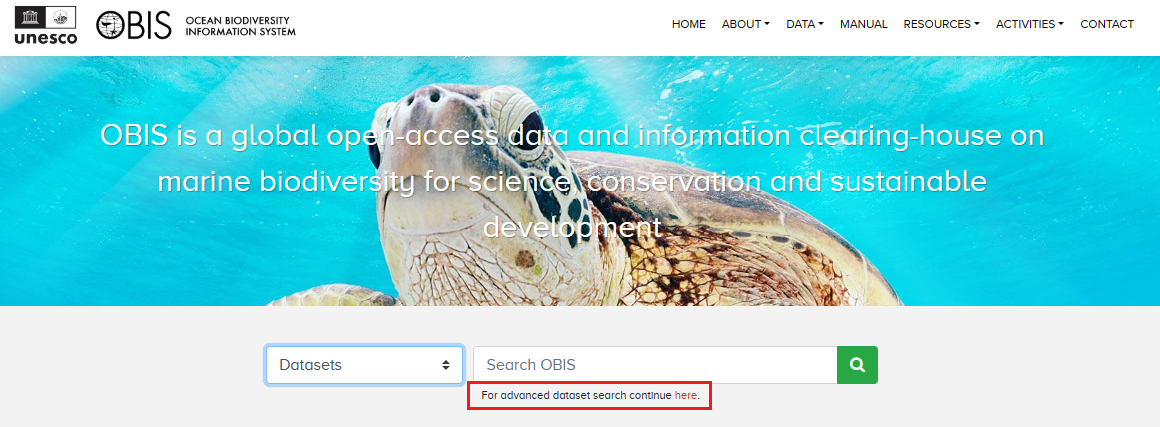
\includegraphics[width=0.9\textwidth,height=\textheight]{images/obis-homepagesearch.png}

}

\caption{\emph{OBIS homepage search, showing where to find the advanced
search link}}

\end{figure}

Regardless if you found a dataset through the homepage or the advanced
Dataset search, you will be able to navigate to individual dataset
pages. For individual dataset pages (instead of aggregate pages for
e.g., a Family) there are three buttons available:

\begin{itemize}
\tightlist
\item
  Report issue - allows you to report any issues with the dataset in
  question
\item
  Source DwC-A - download the dataset as a Darwin Core-Archive file.
  This will provide all data tables as separate files within a zipped
  folder
\item
  To mapper - this will open another browser with the data shown in the
  Mapper
\end{itemize}

\begin{figure}

{\centering 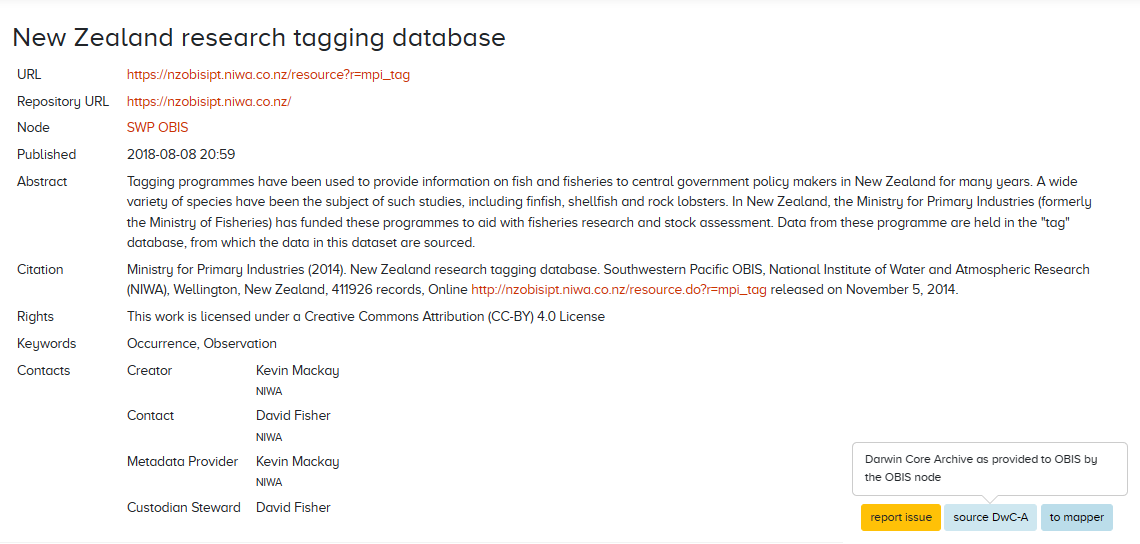
\includegraphics[width=0.9\textwidth,height=\textheight]{images/dataset-DL.png}

}

\caption{\emph{Dataset download}}

\end{figure}

If you searched for aggregate datasets (e.g., all Crustacea records, all
records from OBIS-Canada, etc.), the \texttt{source\ DwC-A} button will
not be available to you. To download these data subsets, you must click
\texttt{to\ mapper} and then \protect\hyperlink{mapper}{download the
data from the Mapper as a CSV}.

\hypertarget{mapper}{%
\section{Mapper}\label{mapper}}

\begin{itemize}
\tightlist
\item
  \url{https://mapper.obis.org}
\end{itemize}

Watch this video demonstration of how to use the Mapper as well as the
OBIS homepage search.

The mapper allows users to visualize and inspect subsets of OBIS data. A
variety of filters are available (taxonomic, geographic, time, data
quality) and multiple layers can be combined in a single view. Layers
can be downloaded as CSV files.

\begin{figure}

{\centering 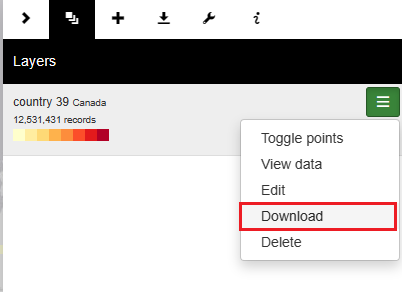
\includegraphics[width=0.6\textwidth,height=\textheight]{images/mapper-DL.png}

}

\caption{\emph{Screenshot demonstrating where how to download a
particular layer}}

\end{figure}

When you download data from the mapper, you will be given the option to
include eMoF and/or DNA Derived Data extensions alongside the Event and
Occurrence data. You must check the boxes of extensions you want to
include in your download.

\begin{figure}

{\centering 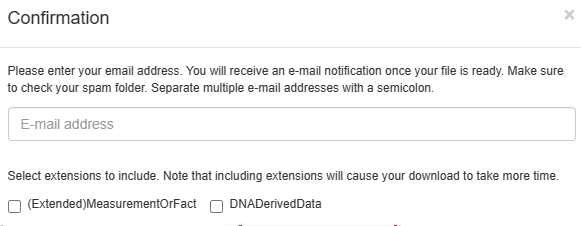
\includegraphics[width=0.7\textwidth,height=\textheight]{images/mapper-extensions.png}

}

\caption{\emph{Screenshot showing the popup confirmation for which
extensions you want to include in your download from the OBIS Mapper}}

\end{figure}

After downloading, you will notice that the Event and Occurrence data is
flattened into one table, called ``Occurrence.csv''. Upon inspecting
this file in your viewer of choice, you will see it contains all 225
possible DwC fields, although not every field will contain data for each
observation. Any extensions you checked will be downloaded as separate
tables.

\hypertarget{r-package}{%
\section{R package}\label{r-package}}

\begin{itemize}
\tightlist
\item
  \url{https://github.com/iobis/robis}
\end{itemize}

The robis R package has been developed to facilitate connecting to the
OBIS API from R. The package can be installed
\href{https://cran.r-project.org/web/packages/robis/index.html}{from
CRAN} or \href{https://github.com/iobis/robis}{from GitHub} (latest
development version). The package documentation includes a function
reference as well as a
\href{https://iobis.github.io/robis/articles/getting-started.html}{getting
started vignette}. As a quick example of what the package can do, you
can obtain raw occurrence data by feeding a taxon name or AphiaID to the
\texttt{occurrence} function.

If you'd like to then download this data, you can simply export R
objects with the \texttt{write.csv} function. For example, if we wanted
to obtain Mollusc data from OBIS:

\begin{Shaded}
\begin{Highlighting}[]
\FunctionTok{library}\NormalTok{(robis)}
\NormalTok{moll}\OtherTok{\textless{}{-}}\FunctionTok{occurrence}\NormalTok{(“Mollusca”)}
\FunctionTok{write.csv}\NormalTok{(moll, “mollusca}\SpecialCharTok{{-}}\NormalTok{obis.csv”)}
\end{Highlighting}
\end{Shaded}

This file will be saved to your working directory (if you are not
familiar with working directories, read
\href{https://bookdown.org/ndphillips/YaRrr/the-working-directory.html}{here}).
After opening the file, you will notice that the fields in the download
do not include every possible field, but instead only those where
information has been recorded by data providers, plus the
\protect\hyperlink{interpreting-downloaded-files-from-obis}{fields added
by OBIS's quality control pipeline}.

To use \texttt{robis} for visualizing and mapping occurrences, see the
\href{dataviz.html}{Visualization} section of the manual.

Watch the video below for a walkthrough of how to use the robis package
to obtain OBIS data.

\hypertarget{api}{%
\section{API}\label{api}}

\begin{itemize}
\tightlist
\item
  \url{https://api.obis.org/}
\end{itemize}

Both the mapper and the R package are based on the
\href{https://api.obis.org/}{OBIS API}, which can also be used to find
and download data. When using the API directly, you can filter by the
following options:

\begin{itemize}
\tightlist
\item
  Occurrence
\item
  Taxon
\item
  Checklist
\item
  Node
\item
  Dataset
\item
  Institute
\item
  Area
\item
  Country
\item
  Facet
\item
  Statistics
\end{itemize}

When you have entered all the information you are interested in
filtering by, scroll down and click the ``Execute'' button. This will
produce a response detailing how many records match your criteria, as
well as information for some of the headers from the data (e.g.,
basisOfRecord, Order, genus, etc.). A download button will be available
for you to download the data as well.

When searching with the API, you may need to know certain identifiers,
including:

\begin{itemize}
\tightlist
\item
  AphiaID - obtainable from the WoRMS page of a taxa of interest
  (e.g.~the AphiaID for
  \href{https://www.marinespecies.org/aphia.php?p=taxdetails\&id=51}{Mollusca}
  would be 51)
\item
  Dataset UUID - can be obtained from the URL on individual dataset
  pages

  \begin{itemize}
  \tightlist
  \item
    E.g.,
    \href{https://obis.org/dataset/5061d21c-6161-4ea2-a8d4-38f8285dfc47}{this
    dataset's} UUID would be 5061d21c-6161-4ea2-a8d4-38f8285dfc47
  \end{itemize}
\item
  Area ID
\item
  Institute ID - this should be the Ocean Expert ID (e.g., the ID for
  \href{https://oceanexpert.org/institution/7532}{NOAA Fisheries
  Service, Southeast Regional Office St.~Petersburg} is 7532)
\item
  OBIS node UUID
\end{itemize}

A short video demonstrating use of the API is shown below.

\hypertarget{full-exports}{%
\section{Full exports}\label{full-exports}}

\begin{itemize}
\tightlist
\item
  \url{https://obis.org/data/access/}
\end{itemize}

To obtain a full export of OBIS data, navigate to the OBIS homepage,
click on Data from the top navigation bar, then select
\href{https://obis.org/data/access/}{Data Access} from the dropdown
menu.

\begin{figure}

{\centering 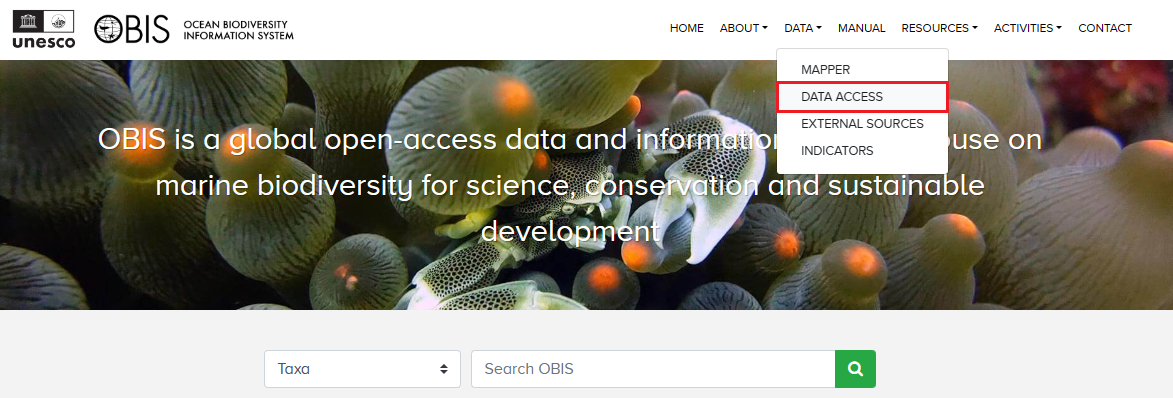
\includegraphics{images/full-export1.png}

}

\caption{\emph{OBIS homepage showing where to navigate to access full
database exports}}

\end{figure}

Here you will be able to download all occurrence records as a CSV or
Parquet file. Note the disclaimer that such exports will not include
measurement data, dropped records, or absence records. As with downloads
from the Mapper, the exported file is a single Occurrence table. This
table includes all provided Event and Occurrence data, as well as 68
fields added by the OBIS Quality Control Pipeline, including taxonomic
information obtained from WoRMS.

\begin{figure}

{\centering 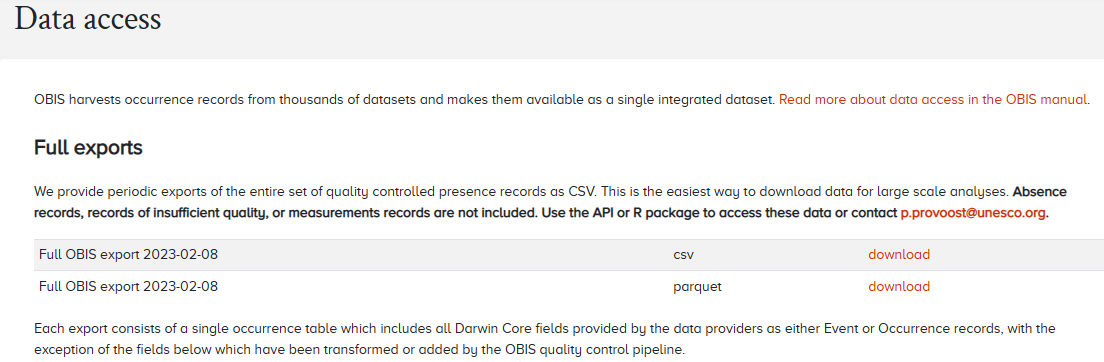
\includegraphics{images/full-export2.png}

}

\caption{\emph{OBIS Data Access page}}

\end{figure}

\hypertarget{finding-your-own-data-in-obis}{%
\section{Finding your own data in
OBIS}\label{finding-your-own-data-in-obis}}

To find your own dataset in OBIS, you can use the same tools as finding
any dataset in OBIS. You have the following options:

\begin{itemize}
\tightlist
\item
  From the \href{https://obis.org/}{OBIS homepage} or the
  \href{https://mapper.obis.org/}{Mapper}, you can search by dataset
  name, species of interest, the OBIS node that you uploaded to, or by
  institute

  \begin{itemize}
  \tightlist
  \item
    Note: When using the Mapper you can combine multiple search criteria
    to help narrow down your search

    \begin{itemize}
    \tightlist
    \item
      E.g., if we wanted to find
      \href{https://obis.org/dataset/80479e14-2730-436d-acaa-b63bdc7dd06f}{this
      dataset} in the Mapper, we could search for OBIS USA under Nodes,
      National Oceanic and Atmospheric Administration, Washington under
      Institutes, and/or Radiozoa under Scientific Name. Then when we
      view the data and scroll down to datasets, the only one listed is
      the one we were interested in
    \end{itemize}
  \end{itemize}
\item
  If you have used the (extended)measurementOrFact extension and have
  measurementType data, you can \href{https://mof.obis.org/}{search by
  the name of your measurementType}, click on the hyperlink for records.
  This will populate a list of datasets that you can scroll through.
\end{itemize}

\hypertarget{how-to-contact-data-provider}{%
\section{How to contact data
provider}\label{how-to-contact-data-provider}}

To contact the data provider, navigate to the page for the individual
dataset in question (e.g.,
\url{https://obis.org/dataset/80479e14-2730-436d-acaa-b63bdc7dd06f}).
Under the ``Contacts'' section, there will be a list of individuals you
can contact. Clicking any name will direct you to your system's default
email program. For example:

\begin{figure}

{\centering 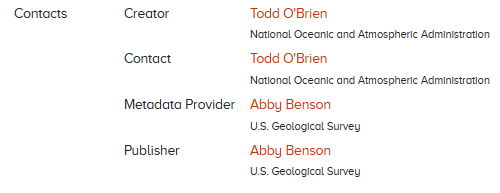
\includegraphics[width=0.7\textwidth,height=\textheight]{images/contact-dataprovider.png}

}

\caption{\emph{Example of contact section on a dataset homepage access
via the OBIS search}}

\end{figure}

If you are the node manager and need to contact the data provider about
a particular dataset, contact information should be provided in the
metadata and you can contact them from information provided.

\hypertarget{interpreting-downloaded-files-from-obis}{%
\section{Interpreting downloaded files from
OBIS}\label{interpreting-downloaded-files-from-obis}}

In general, the field names you will see when you download data from
OBIS are the same as those seen during the data formatting and
publishing process. When you download data from the
\href{https://mapper.obis.org/}{Mapper} you will see all 225 possible
Darwin Core fields.

Downloading data from an IPT or full export will include only the fields
provided by the data provider, formatted as one Occurrence file (or
separate files for individual datasets). Some fields are added through
the OBIS quality control pipeline, including taxonomic information from
WoRMS and the fields \texttt{flags}, \texttt{bathymetry}, and
\texttt{dropped}. As mentioned in the \href{dataquality.html}{Quality
Control section}, the fields \texttt{flags} and \texttt{dropped} will
list quality control issues or if the record was dropped, respectively.
Details and definitions for all fields added by the OBIS QC pipeline can
be found \href{https://obis.org/data/access/}{here}.

For a full list of the other Darwin Core terms and their definitions
included in downloads, please reference the
\href{https://dwc.tdwg.org/terms/}{Darwin Core reference guide}.

\part{Data Visualization and Analysis}

\hypertarget{data-visualization}{%
\chapter{Data Visualization}\label{data-visualization}}

\hypertarget{example-notebooks-using-data-from-obis}{%
\section{Example notebooks using data from
OBIS}\label{example-notebooks-using-data-from-obis}}

Here are a few R notebooks showcasing the robis package:

\begin{itemize}
\tightlist
\item
  \href{https://iobis.github.io/notebook-windfarms/}{Data exploration of
  wind farm monitoring datasets in OBIS}
\item
  \href{https://iobis.github.io/notebook-mwhs/}{Diversity of fish and
  vulnerable species in Marine World Heritage Sites based on OBIS data}
\item
  \href{https://iobis.github.io/notebook-reeffish/}{Data exploration -
  Stratified random surveys (StRS) of reef fish in the U.S. Pacific
  Islands}
\item
  \href{https://iobis.github.io/notebook-dnaderiveddata/}{DNADerivedData
  extension data access}
\item
  \href{https://iobis.github.io/notebook-cclme/}{Canary Current LME}
\end{itemize}

Here are others that may be of interest:

\begin{itemize}
\tightlist
\item
  \href{https://iobis.github.io/notebook-diversity-indicators/}{Diversity
  indicators using OBIS data}
\item
  \href{https://iobis.github.io/notebook-ospar/}{OBIS species richness
  for OSPAR}
\item
  \href{https://iobis.github.io/notebook-deepdata/}{Quality control of
  ISA data}
\item
  \href{https://iobis.github.io/notebook-gridded-data/}{Accessing
  gridded data}
\end{itemize}

\hypertarget{obisindicators-calculating-visualizing-spatial-biodiversity-using-data-from-obis}{%
\section{obisindicators: calculating \& visualizing spatial biodiversity
using data from
OBIS}\label{obisindicators-calculating-visualizing-spatial-biodiversity-using-data-from-obis}}

\href{https://marinebon.org/obisindicators/index.html}{obisindicators}
is an R library developed during the
\href{https://ioos.github.io/ioos-code-sprint/}{2022 IOOS Code Sprint}.
The purpose was to create an ES50 diversity index within hexagonal grids
following the
\href{https://iobis.github.io/notebook-diversity-indicators/}{diversity
indicators notebook} by Pieter Provoost linked above. The package
includes several examples, limited to 1M occurrences, that demonstrate
uses of the package.

\begin{figure}

{\centering 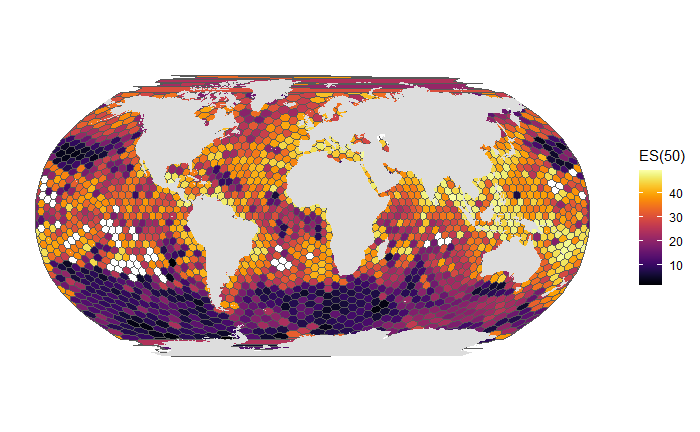
\includegraphics{./images/all_data.png}

}

\caption{screenshot}

\end{figure}

\part{Additional Resources}

\hypertarget{other-resources}{%
\chapter{Other Resources}\label{other-resources}}

In this section we highlight useful resources created by collaborators
and other community members.

\hypertarget{mbon-pole-to-pole-tutorial}{%
\section{MBON Pole to Pole Tutorial}\label{mbon-pole-to-pole-tutorial}}

\begin{itemize}
\tightlist
\item
  \url{https://www.youtube.com/watch?v=teJhfsSWonE}
\end{itemize}

This tutorial was created by the
\href{https://marinebon.org/p2p/index.html}{MBON Pole to Pole project}
to help guide people through the process of transforming datasets to
Darwin Core using
\href{https://marinebon.org/p2p/methods_data_science.html}{tools} MBON
Pole to Pole has developed.

\hypertarget{ioos-darwin-core-guide}{%
\section{IOOS Darwin Core Guide}\label{ioos-darwin-core-guide}}

\begin{itemize}
\tightlist
\item
  \url{https://ioos.github.io/bio_data_guide/}
\end{itemize}

This book contains a collection of examples and resources related to
mobilizing marine biological data to the
\href{https://dwc.tdwg.org/}{Darwin Core standard} for sharing though
\href{https://obis.org/}{OBIS}. This book has been developed by the
\href{https://github.com/ioos/bio_data_guide/blob/main/README.md}{Standardizing
Marine Biological Data Working Group (SMBD)}. The working group is an
open community of practitioners, experts, and scientists looking to
learn and educate the community on standardizing and sharing marine
biological data.

\hypertarget{emodnet-biology}{%
\section{EMODnet Biology}\label{emodnet-biology}}

\begin{itemize}
\tightlist
\item
  \url{https://classroom.oceanteacher.org/course/view.php?id=430}
\end{itemize}

Contributing Datasets to EMODnet Biology is a course hosted on
\href{https://classroom.oceanteacher.org/}{Ocean Teacher Global Academy
(OTGA)}, developed by members of the
\href{https://emodnet.ec.europa.eu/en}{European Marine Observation and
Data Network}. The course prepares users to format, publish, and perform
quality control checks on datasets according to Darwin Core standards.
While targeted at EMODnet Biology users, this course has significant
overlap in how to prepare datasets for OBIS and is useful for those
unfamiliar with OBIS standards. Note, an account with OTGA is required
to access the course.

\hypertarget{template-generators}{%
\section{Template Generators}\label{template-generators}}

There is an
\href{https://www.nordatanet.no/aen/template-generator/config\%3DDarwin\%20Core}{Excel
template generator} developed by Luke Marsden \& Olaf Schneider as part
of the Nansen Legacy project. It allows the creation of Event or
Occurrence core templates, with an optional eMoF extension. Note this
template generator is aimed at GBIF users, so make sure to account for
and include required OBIS terms.

There is also an
\href{https://zenodo.org/record/6453921\#.Y9KsQkHMKmU}{Excel to Darwin
Core macro tool} developed by GBIF Norway that you can download for use
in Microsoft Excel. This macro can help you set up Event, Occurrence,
and eMoF tables by selecting all relevant DwC fields from a list, or by
importing data from another spreadsheet. It allows for auto-generation
of identifiers (e.g.~eventID, occurrenceID) if macros are enabled, and
can also auto-populate the eMoF when measurement fields in the
Occurrence table are populated.



\end{document}
